% 2017/01/01 Software textbook - MATLAB

\documentclass
%[draft]{book}
{book}
\usepackage{amsmath, amssymb, float, subfigure, epsfig}
\usepackage{amsthm}
\usepackage{graphicx}
%\usepackage{hangul}
\usepackage{color}


%=========================================================
\newcommand{\defh}{\hspace{1mm}$\hat{}$\hspace{1mm}}
\newcommand{\defhh}{\hspace{.3mm} \hat{} \hspace{.3mm}}
\newcommand{\vs}{\par \vspace{.3in}}
\newcommand{\vv}{\par \vspace{.1in}}
\newcommand{\hh}{\hspace{.1in}}
\newcommand{\vn}{\vv\noindent}
\newcommand{\nnline}{\vn}
\newcommand{\maplep}{\vv [ \ $>$\ }
\newcommand{\matlabp}{\vv $\gg$\ }
\newcommand{\doublespace}{\addtolength{\baselineskip}{.13\baselineskip}}

%\newtheorem{example}{Example}
\newtheorem{example}{예제}
\newtheorem{problem}{Problem}
\newtheorem{Theorem}{Theorem}{}
\newenvironment{Proof}{\par {\noindent \it Proof.}}{}
%=========================================================

%=========================================================
\floatstyle{ruled}
\newfloat{alg}{tnp}{lop}[chapter]
\floatname{alg}{ALGORITHM}
%=========================================================

\begin{document}

\frontmatter

\title{\bf{Learning MATLAB with Linear Algebra}}

\author{Soomin Jeon and Chang-Ock Lee\\ \\ \\ \\ \\ \\ \\ \\ \\ \\ \\ \\ \\ \\ \\ \\ \\ \\ \\ \\ \\ \\ \\ \\ \\ \\
 Department of Mathematical Sciences\\KAIST}
\date{2017}

\mainmatter
\maketitle



\theoremstyle{remark}
\newtheorem*{sol}{\bf\textit{Solution{}}}{}
\newtheorem*{outputs}{\bf\textit{MATLAB results}}
\newtheorem{prob}{\bf{Problem}}
\newtheorem{exer}{\bf{Exercise}}
\numberwithin{exer}{chapter} % important bit


\graphicspath{{./fig-matlab/}}

\tableofcontents
\chapter{Matlab Basics and Programming }
Matlab is a commercial program\footnote{The homepage is www.mathworks.com.} which provides an integrated environment for ``Matrix Laboratory". Matlab is one of many softwares used most ubiquitously in areas of mathematics and engineering. Matlab is very compatible with areas of fields which require numerical simulations because the built-in functions and m-files are based on the standard library LIN-PACK and EISPACK\footnote{One can obtain the source files from www.netlib.org}.

\vv The filenames of Matlab files and script files always end in ``.m". The program is very convenient to use because almost all of the structures are composed of matrices. In addition, the graphic processing is set so that the numerical analysis results are expressed conveniently.

\vv One can get explanation regarding Help by typing
\matlabp\texttt{\textbf{help}} \vn in the Matlab command window, and one can get explanations regarding every available Matlab functions. For information regarding a specific command, type  \matlabp\texttt{\textbf{help command\_name}} \vn For instance, \matlabp\texttt{\textbf{help fft}} \vn gives explanation for \texttt{\textbf{fft}} command. To see the explanation in document form with Hypertext structure, use {\tt doc} instead of {\tt help}.

\vv This chapter deals with basic usage of Matlab and programming. 
%For reference, basic Matlab command list is in appendix %\ref{A-Matlab}.

\section{Basic Command}
\subsection{Matrix}
Matlab has many different types of built-in matrices. For instance, let us try to make a $7 \times 7$ matrix with random numbers in each entries. \vv \texttt{\textbf{$\gg$ rand(7)}} \vn We can also make a random matrix with a different number of columns and rows by, for example, \matlabp\texttt{\textbf{rand(2,5)}} \vn For more explanations regarding the function rand, use help or doc command. Another specific matrix, Hilbert matrix, is a typical example used in numerical analysis. \matlabp\texttt{\textbf{hilb(5)}} \matlabp\texttt{\textbf{help hilb}} \vn $5 \times 5$ magic square can be made with the following command. \matlabp\texttt{\textbf{magic(5)}} \matlabp\texttt{\textbf{help magic}} \vn Magic square is a square matrix with the summation of the entries in the row, column, and diagonal all equal. This property of magic square will be explored in subsection 1.3 %\ref{Matlab-ft}
 using matrix multiplication. Many types of matrices used in numerical analysis can be made using built-in functions. \matlabp\texttt{\textbf{eye(6)}} \matlabp\texttt{\textbf{zeros(4,7)}} \matlabp\texttt{\textbf{ones(5)}} \vn Not only limited to these built-in matrices, one can make different matrices in any form. \matlabp\texttt{\textbf{[1 2 3 5 7 9]}} \matlabp\texttt{\textbf{[1, 2, 3; 4, 5, 6; 7, 8, 9]}} \matlabp\texttt{\textbf{[1 2 RET 3 4 RET 5 6]}} \vn Here {\tt RET} means one must press the "return key". Matlab grammatical system allows for easy usage of block matrices. \matlabp\texttt{\textbf{[eye(2); zeros(2)]}} \matlabp\texttt{\textbf{[eye(2); zeros(3)]}} \matlabp\texttt{\textbf{[eye(2), ones(2,3)]}} \vn The second example above gives an error. Why is that?

\subsection{Variable}
Matlab has built-in variables, such as {\tt pi}, {\tt eps}, and {\tt ans}. \matlabp\texttt{\textbf{pi}} \matlabp\texttt{\textbf{eps}} \matlabp\texttt{\textbf{help eps}} \vn \texttt{\textbf{who}} is a command which tells us which variables are currently being used. In addition, one can see which variables are being used in the Workspace. \matlabp\texttt{\textbf{who}} \matlabp\texttt{\textbf{help who}} \vn \texttt{\textbf{ans}} is a variable which has the value of the last calculated results that was not assigned a variable. \matlabp\texttt{\textbf{magic(6)}} \matlabp\texttt{\textbf{ans}} \matlabp\texttt{\textbf{x = ans}} \matlabp\texttt{\textbf{x = [x, eye(6)]}} \matlabp\texttt{\textbf{x}} \matlabp\texttt{\textbf{who}} \vn Since a new variable x has been created, x is a variable being used. In order to delete a variable, use the following command. \matlabp\texttt{\textbf{clear x}} \matlabp\texttt{\textbf{x}} \matlabp\texttt{\textbf{who}} \vn In order to erase all variables, use \matlabp\texttt{\textbf{clear}} \vn or \matlabp\texttt{\textbf{clear all}} \vn Use \texttt{\textbf{help}} or {\tt doc} to figure out the difference between the two.

\subsection{Functions} \label{Matlab-ft}
Let us try the following command. \matlabp\texttt{\textbf{a = magic(4)}} \vn Now let us find the transpose of a \matlabp\texttt{\textbf{a'}} \vn If {\tt a} was a complex matrix, then Matlab would calculate the conjugate transpose, not simply a transpose. 

\vv Let us explore other arithmetic operations. \matlabp\texttt{\textbf{3*a}} \matlabp\texttt{\textbf{-a}} \matlabp\texttt{\textbf{a + (-a)}} \matlabp\texttt{\textbf{b = max(a)}} \matlabp\texttt{\textbf{max(b)}} \vn Some Matlab functions may have output with more than one values. If one uses \texttt{\textbf{max}} on matrix, then the output is maximum of each column and the indices of the row that contains that maximum. For vector case, the maximum value and the index of that value is presented. \matlabp\texttt{\textbf{[m, i] = max(b)}} \matlabp\texttt{\textbf{[m, i] = min(a)}}

\vn Let us try matrix multiplication in order to verify the ``magic" of magic square.  \matlabp\texttt{\textbf{A = magic(5)}}  \matlabp\texttt{\textbf{b = ones(5,1)}}  \matlabp\texttt{\textbf{A*b}}  \matlabp\texttt{\textbf{v = ones(1,5)}}  \matlabp\texttt{\textbf{v*A}}

\vv In Matlab, dot in front of an operation means entry-by-entry operation. In matrix multiplication, {\tt a.*b} is different from usual matrix multiplication in that the multiplication is done entry-by-entry.  \matlabp\texttt{\textbf{b = 2*ones(4)}}  \matlabp\texttt{\textbf{a.*b}}  \matlabp\texttt{\textbf{a*a}}  \matlabp\texttt{\textbf{a\defh 2}}  \matlabp\texttt{\textbf{a.\defh 2}} \vn The followings are many different arithmetic operations related to matrix.  \matlabp\texttt{\textbf{triu(a)}}  \matlabp\texttt{\textbf{tril(a)}}  \matlabp\texttt{\textbf{diag(a)}}  \matlabp\texttt{\textbf{diag(diag(a))}}  \matlabp\texttt{\textbf{c = rand(4,5)}}  \matlabp\texttt{\textbf{size(c)}}  \matlabp\texttt{\textbf{[m,n] = size(c)}}  \matlabp\texttt{\textbf{m}}  \matlabp\texttt{\textbf{d = .5-c}}

\vv Typically, Matlab commands are used for scalar, but there are many functions that can be applied for both scalars and matrices.  \matlabp\texttt{\textbf{sin(d)}}  \matlabp\texttt{\textbf{exp(d)}}  \matlabp\texttt{\textbf{log(d)}}  \matlabp\texttt{\textbf{abs(d)}}

\vv There are functions which translates decimal valued numbers into integers in Matlab. {\tt round}, {\tt fix}, {\tt ceil}, and {\tt floor} are some of these. For instance,  \matlabp\texttt{\textbf{f = [-.5 .1 .5]}}  \matlabp\texttt{\textbf{round(f)}}  \matlabp\texttt{\textbf{fix(f)}}  \matlabp\texttt{\textbf{ceil(f)}}  \matlabp\texttt{\textbf{floor(f)}}

\subsection{Logic operation}
Let us think of 1 as ``true", and 0 as ``false" in this subsection. \&, $|$, and $\sim$ are logic operations which mean ``and", ``or", and ``not", respectively. == is a logic operation which means equal.  \matlabp\texttt{\textbf{a = [1 0 1 0]}}  \matlabp\texttt{\textbf{b = [1 1 0 0]}}  \matlabp\texttt{\textbf{a == b}}  \matlabp\texttt{\textbf{a <= b}}  \matlabp\texttt{\textbf{$\sim$a}}  \matlabp\texttt{\textbf{a \$ b}}  \matlabp\texttt{\textbf{a \$ $\sim$a}}  \matlabp\texttt{\textbf{a $|$ b}}  \matlabp\texttt{\textbf{a $|$ $\sim$a}} \vn There is a comand named {\tt any} that checks whether the matrix has at least one non-zero entry or not. Not only that, there is also a command named {\tt all} that checks whether all the entries in the matrix are non-zero or not.  \matlabp\texttt{\textbf{a}}  \matlabp\texttt{\textbf{any(a)}}  \matlabp\texttt{\textbf{c = zeros(1,4)}}  \matlabp\texttt{\textbf{d = ones(1,4)}}  \matlabp\texttt{\textbf{any(c)}}  \matlabp\texttt{\textbf{all(a)}}  \matlabp\texttt{\textbf{all(d)}}  \matlabp\texttt{\textbf{e = [a', b', c', d']}}  \matlabp\texttt{\textbf{any(e)}}  \matlabp\texttt{\textbf{all(e)}}  \matlabp\texttt{\textbf{any(all(e))}}

\subsection{Colon}
Matlab provides a useful command for producing and dividng a matrix.  \matlabp\texttt{\textbf{x = -2:1}}  \matlabp\texttt{\textbf{length(x)}}  \matlabp\texttt{\textbf{-2:.5:1}}  \matlabp\texttt{\textbf{-2:.2:1}}  \matlabp\texttt{\textbf{a = magic(5)}}  \matlabp\texttt{\textbf{a(2,3)}} \vn Now let us try using colon to select specific rows and columns of {\tt a}.  \matlabp\texttt{\textbf{a(2,:)}} \matlabp\texttt{\textbf{a(:,3)}} \matlabp\texttt{\textbf{a(2:4,:)}} \matlabp\texttt{\textbf{a(:,3:5)}} \matlabp\texttt{\textbf{a(2:4,3:5)}} \matlabp\texttt{\textbf{a(1:2:5,:)}} \vn In addition, one can freely use row or column vectors in a matrix. \matlabp\texttt{\textbf{a(:,[1 2 5])}} \matlabp\texttt{\textbf{a([2 5],[2 4 5])}}

\vn And one can use assignment statements using vectors and matrices. \matlabp\texttt{\textbf{b = rand(5)}} \matlabp\texttt{\textbf{b([1 2],:) = a([1 2],:)}} \matlabp\texttt{\textbf{a(:,[1 2]) = b(:,[3 5])}} \matlabp\texttt{\textbf{a(:,[1 5]) = a(:,[5 1])}} \matlabp\texttt{\textbf{a = a(:,5:-1:1)}} \vn All of these are simple Matlab functions and examples of matrix multiplication. More functions can be found in the appendix \ref{A-Matlab}.

\subsection{Other features}
The default setting for Matlab is that the decimals are expressed up to 4 decimal digits. Even though the actual calculation is done up to 16 decimal digits, it is rounded and then expressed. The command \matlabp\texttt{\textbf{format long}} \vn changes so that all 16 decimal digits are displayed. And, \matlabp\texttt{\textbf{format short}} \vn changes back to the default setting. Of course, one can display scientific constants long or short, however one wishes, by using the following command \matlabp\texttt{\textbf{format short e}} \matlabp\texttt{\textbf{format long e}}

\vv It is not necessary to always display all the calculated values on the screen. If one attaches semicolon(;) at the end of the command, then calculation will proceed, but the values will not be displayed, just like the colon in Maple.

\vv Sometimes, a lot of time is spent on making matrices in Matlab session, and one might need to use these matrices next time. One can use Matlab command \matlabp\texttt{\textbf{save filename}} \vn to make a file named \texttt{\textbf{filename.mat}} that saves all the variable values made in the current session. If one does not wish to save all the variable values, then one can use \matlabp\texttt{\textbf{save filename x y z}} to save only variable {\tt x,y,z} in \texttt{\textbf{filename.mat}}. These saved variables can be reused next time using the command \matlabp\texttt{\textbf{load filename}}

\vv There are times when one must record all the keyboard inputs and results in Matlab session. The following command allows one to record all the process except for graphs. \matlabp\texttt{\textbf{diary filename}} \vn produces a file named \texttt{\textbf{filename}} and starts the record. \matlabp\texttt{\textbf{diary off}} \vn stops the record, \matlabp\texttt{\textbf{diary on}} \vn restarts the record. These processes are saved in text files, so one can edit them.

\section{Programming in Matlab}
Matlab is a language, with which one is able to program, just like Maple. A person who wants to write the files can easily do so by using .m files toy write a program and execute it. If one wrote {\tt myfile.m}, one can execute {\tt myfile.m} by using the command {\tt myfile}, just like other Matlab commands. Matlab is an interpreter language, so one can execute a written program without compiling.

\subsection{Assignment Statement}
Assignment means one can assign a value to a variable. In other words, {\tt x=a} means that one is assigning the value {\tt a} to the variable {\tt x}. Let us see the following simple program which uses assignment statement.

\vv
\begin{center}
\fbox{\parbox{10.5cm}{\begin{center}
\parbox{9.5cm}{\tt function r=mymod(a,d)\\ \\
\% r=mymod(a,d). If a and d are integers, then \\
\% r is the integer remainder of a after\\
\% division by d. If a and d are integer matrices, \\
\% then r is the matrix of remainders after division \\
\% by corresponding entries. Compare with REM.\\ \\
r=a-d.*floor(a./d);} \end{center} }}\end{center} \vn Make the above {\tt mymod.m} file, and assign an integer value to {\tt a} and {\tt d}. Then, if one uses

\matlabp \texttt{\textbf{mymod(a,d)}}

\vn it is executed as if it were a built-in Matlab command. Let us enter the following command.

\matlabp \texttt{\textbf{help mymod}}

\vn Then the 5-lined information above that start with \% will show up. \% means that the statements that come after it are ignored when a program is executed. When help command is executed in Matlab, the information on the uppermost part of the announced part of the function is displayed. Using this method, the help command provides a help function that let us know the properties of the function quickly. Let us enter the following.

\matlabp\texttt{\textbf{type mymod}}

\vn This command displays the entire details of the file on the screen for convenient reading. Now let us examine the details of {\tt mymod.m}. The first row corresponds to ``function announcement statement". In here, name of the file(always the same as the file name without m), input variable(In this case, {\tt a} and {\tt d}), and output variable({\tt r}) are announced. The next is the `help" aforementioned. Last, the middle part of the program is displayed on the screen. The variable {\tt r} is assigned the value {\tt a-d.*floor(a./d)}. Out of the operations on the right hand side, ``." means entry-by-entry operation. Last, ``;" means that until the last part of the execution, the result is blocked from being printed on the screen. Try executing the program after deleting ``;". A quite different result will be printed.

\subsection{Conditional Statement}
Conditional statement has the following structure. \vv

\texttt{\textbf{if <condition>, <program> end}} \vn \texttt{\textbf{<condition>}} above is a MATLAB function, but it is not a must to have values only 0 and 1. In the conditional statement, \texttt{\textbf{<program>}} is executed only when \texttt{\textbf{<condition>}} has a non-zero value, and proceeds to the next. Let us not forget that {\tt a==b} and {\tt a<=b} are functions perceived as having values 0 or 1. Often, conditional statements have the following form. \vv \texttt{\textbf{if <condition1>, <program1> else <program2> end}} \vn In this case, if {\tt <condition1>} has the value 0, then {\tt <program2>} is performed. There is another form \vv \texttt{\textbf{if <condition1>, <program1>}} \par \texttt{\textbf{elseif <condition2>, <program2>}} \par \texttt{\textbf{end}} In this case, if {\tt <condition1>} is non-zero, then {\tt <program1>} is performed, if {\tt <condition1>} is 0 and {\tt <condition2>} is non-zero, then {\tt <program2>} is performed. In other cases, the program exits the conditional statement and proceeds to the next. The following is a simple program that uses conditional statement. \vv
\begin{center}
\fbox{\parbox{10.5cm}{\begin{center}
\parbox{9.4cm}{\tt function b=even(n)\\ \\
\% b=even(n). If n is an even integer, then b=1 \\
\% otherwise b=0 \\ \\
if mymod(n,2) == 0\\
\phantom{ab}b=1; \\
\phantom{ab}else b=0; \\
end} \end{center} }}\end{center}

\subsection{For Loop}
For loop has the following structure.

\vv \texttt{\textbf{for i=1:n, <program>, end}} \vn Depending on the value of {\tt i}, \texttt{\textbf{<program>}} is repeatedly executed each time. Let us introduce some simple program. The first is matrix multiplication. \vv
\begin{center}
\fbox{\parbox{10.5cm}{\begin{center}
\parbox{10.2cm}{\tt function c=add(a,b)\\ \\
\% c=add(a,b). This is the function which adds \\
\% the matrices a and b. It duplicates the MATLAB \\
\% function a+b.\\ \\
$[$m,n$]$ = size(a);\\
$[$k,l$]$ = size(b);\\
if m$\sim$=k $|$ n$\sim$=l, \\
\phantom{ab}r='ERROR using add: matrices are not the same size',\\
\phantom{ab}return,\\
end \\
c=zeros(m,n); \\
for i=1:m,\\
\phantom{ab}for j=1:n,\\
\phantom{ab}\phantom{ab}c(i,j)=a(i,j)+b(i,j);\\
\phantom{ab}end \\
end} \end{center} }}\end{center}

\vn The next is a program related to matrix multiplication. \vv

\begin{center}
\fbox{\parbox{10.5cm}{\begin{center}
\parbox{9.5cm}{\tt function c=mult(a,b)\\ \\
\% c=mult(a,b). This is the matrix product of  \\
\% the matrices a and b. It duplicates the MATLAB  \\
\% function c=a*b.\\ \\
$[$m,n$]$=size(a);\\
$[$k,l$]$=size(b);\\
if n$\sim$=k  \\
\phantom{ab}r='ERROR using mult: matrices are not compatible \\
\phantom{ab}\phantom{ab}for multiplication',\\
\phantom{ab}return,\\
end \\
c=zeros(m,l); \\
for i=1:m,\\
\phantom{ab}for j=1:l,\\
\phantom{ab}\phantom{ab}for p=1:n,\\
\phantom{ab}\phantom{ab}\phantom{ab}c(i,j)=c(i,j)+a(i,p)*b(p,j);\\
\phantom{ab}\phantom{ab}end \\
\phantom{ab}end \\
end} \end{center} }}\end{center} \vn  Let us look carefully at the conditional statement after the {\tt size} statement in both programs. It is there to print error message. In {\tt add} case, adding matrices with different dimensions results in printing error message, and in {\tt mult} case, if the dimension of the column of the left matrix and the dimension of the row of the right column do not match, error message prints. If there is an error even when there is no such error messages, then MATLAB will print a strange calculation result. Observe the single quotation marks in the error message part. The sentence indicated by the quotation marks is regarded as text and is displayed as a value of the variable {\tt r}. After the error message is the return command. This is an instruction statement which tells us to return back to the function or prompt that called {\tt add} or {\tt mult}. Return command is very useful in error message statement.

\vv {\tt i} in the next loop statement

\vv \texttt{\textbf{for i=1:n, <program>, end}} \vn can be handled in many different ways in the program. There is no problem in writing a vector in place of {\tt 1:n} in MATLAB. In the case of loop statement

\vv \texttt{\textbf{for i=[2,4,5,6,10], <program>, end}} \vn the program will be executed 5 times repeatedly, with i having the values $2,4,5,6,10$ each time. The developers of MATLAB went further. It's possible to use vector, but what about matrix? Thus the loop statement like the following

\vv \texttt{\textbf{for i=magic(7), <program>, end}} \vn is also possible. This program will be executed 7 times (the dimension of the column), with the variable {\tt i} being the column of {\tt magic(7)} each time.

\subsection {While Loop Statement}
While loop statement takes the following form

\vv \texttt{\textbf{while <condition>, <program>, end}}

\vn \texttt{\textbf{<condition>}} becomes MATLAB function, just like it did in conditional statement. The program keeps executing as long as \texttt{\textbf{<condition>}} has non-zero value. However, there is a risk in using while statement because there is no way to forcefully terminate the while statement. Next is a simple program using a while statement. \vv
\begin{center}
\fbox{\parbox{10.5cm}{\begin{center}
\parbox{8.2cm}{\tt function l=twolog(n) \\ \\
\% l=twolog(n). l is the floor of the base 2 \\
\% logarithm of n.  \\ \\
l=0; \\
m=2; \\
while m<=n\\
\phantom{ab}l=l+1; \\
\phantom{ab}m=2*m; \\
end} \end{center} }}\end{center}

\subsection{Recursion}
Recursion means that the function calls upon itself. Next is a simple example that uses recursion. \vv
\begin{center}
\fbox{\parbox{10.5cm}{\begin{center}
\parbox{10cm}{\tt function y=twoexp(n) \\ \\
\% y=twoexp(n). This is a recursive program for \\
\%\phantom{ab}\phantom{ab}computing \\
\% y=2\defh n. The program halts only if n is a nonnegative \\
\%\phantom{ab}\phantom{ab}integer. \\ \\
if n==0, y=1;\\
\phantom{ab}else y=2*twoexp(n-1); \\
end} \end{center} }}\end{center} \vn Many recursive programs consist of conditional statement just like this program. The condition {\tt n==0} is the basic part of recursion, and it is the only way for the program to restrict itself from calling itself up. The ``else" part is the part that shows the recursion. Let us take note on how {\tt twoexp(n-1)} is executed in a program that calculates {\tt twoexp(n)}. The principle is calling upon smaller number {\tt n-1}, and continuing this until n=0 is called upon. Successful recursion means continuously calling upon smaller number.

\vv However, there are many dangers in using recursion. First, just like while loop statement, the function can continuously call itself up. Second, although it can be stopped, it might calculate unneccesarily, wasting time, and third, while the recursive program is executing, extra memory is required. In massive calculation, the memory storage is crucial, and it must not be unnecessarily wasted. Then, with all these negative sides, why is recursion used? Actually, users who are familiar with using recursive programs can utilize its merits while avoiding these problems. When using recurisve function, one can program easier than when one does not use recursive function.

\subsection{Other Variety of Programs}
One can use matrix-valued functions as conditional statement or conditions of loop statement. In other words, conditions can have matrices such as {\tt ones(2)}, {\tt zeros(2)}, or {\tt eye(2)} in them. If {\tt <condition> = eye(2)} in the following program, how will this program execute?\vv
\texttt{\textbf{if <condition>, <program1>,}}
\par \texttt{\textbf{else <program2>, end}}
\vn Here, {\tt <program1>} is executed when all the entries in {\tt <condition>} is non-zero. Hence, {\tt <program1>} is executed if {\tt <condition>} is {\tt magic(2)}, and {\tt <program2>} is executed if {\tt <condition>} is {\tt eye(2)}.

\vv Now let us predict how the following program will be executed. \vv
\texttt{\textbf{if A $\sim$= B, <program>, end}} \vn Here, {\tt <program>} will only be executed when the entries of {\tt A} and {\tt B} are all different. If we wanted to execute {\tt <program>} even when only one entry of {\tt A} and {\tt B} are different, then how can we do this? There are many ways, but first, we can do \vv \texttt{\textbf{if A == B, else $<$program$>$, end}} \vn With this program, the ``else" part will be executed when at least one entry of {\tt A} and {\tt B} is different. For a different way, we can use {\tt A==B} as {\tt all(all(A==B))} to transform it into binary function. The inner {\tt all} will produce a binary vector with all the entries as 1 if the {\tt i}-th column of {\tt A} and the {\tt i}-th column of {\tt B} are the same. If all the entries of this vector is 1, then the outer {\tt all} will produce 1. Therefore, if at least one entry of {\tt A} and {\tt B} is different, then {\tt all(all(A==B))=0}. Therefore, the following program \vv \texttt{\textbf{if $\sim$all(all(A==B)), <program>, end}} \vn will be executed as we want.

\vv Very similar method is also used in while loop statement.
\vv \texttt{\textbf{while <condition>, <program>, end}} \vn With this program, when {\tt <condition>} takes a matrix value, the program is continuously executed if all the entries are non-zero, and the program exits the loop statement if at least one of the entry is 0.

\vv The following program uses many conditional statements at the same time. Let us predict how this program is executed.  \vv \texttt{\textbf{if <condition1> \& <codition2>,}}
\par \texttt{\textbf{<program>, end}} \vn Of course, the program is executed when both {\tt <condition1>} and {\tt <condition2>} are non-zero. But, does this program always work without any problems? In reality, there are times when {\tt <condition1> = 0} and {\tt <condition2>} causes an error during the execution of a program.  For instance, this happens in the following program.  \vv \texttt{\textbf{if i $<=$ m \& A(i,j)==0, <program>, end}} \vn Here, {\tt m} is the dimension of the column of {\tt A}. If {\tt i>m}, then we would like the program to proceed on. However, the error message will be displayed on the screen because of {\tt A(i,j)} part. To avoid this, one can change the conditional statement as follows. \vv \texttt{\textbf{if i$<=$m,}}
\par
 \quad \texttt{\textbf{if A(i,j)==0,}} \par
\qquad \texttt{\textbf{<program>}} \par \quad
\texttt{\textbf{end}} \par \texttt{\textbf{end}}

\subsection{Script}
Script is m-file without function declaration statement and executes differently from m-file defined by function. Let us assume {\tt x} is one of the variable in use this session. If we write a program using a function(-defined) file, and we use {\tt x} in the program even if {\tt x} is not an input variable of the function, then the program does not use the value of {\tt x} that was defined during the session, but it takes on the value that was locally allocated in the program. Furthermore, the program does not change the value of {\tt x} in the session. Therefore, during the execution of function file, it is very convenient in that one does not need to take heed of the variable declared in the session, and this is because of the function that was declared. If there is no part about the declaration, then that script is regarded as a continuous part of the session. Hence, if a used variable is changed in the script during the session, then the variable is changed for the entire session.

\subsection{Proposal for Better Programming}
Pay special attention to the following details when programming with MATLAB. Of course, these details can be applied with not only Matlab, but also for programming in Maple as well.

\begin{enumerate}
\item Just like the examples until now, it is recommended to use indent while programming. This way, it is easier to read, easier to find  grammatical errors, and easier to think of programming in group.

\item Be precise with writing footnote. This is because there can be times when one cannot understand the program that he or she has written. If one uses \% in a sentence, then everything after \% in that line becomes footnote.

\item Insert the error message just like the examples above. These error messages are very helpful when debugging.

\item Always structuralize the output as the same as the form of input of other functions. For example, if the form of output of a program is ``yes-no", then change it to 1 or 0 instead of ``yes" and ``no". This way, they can be used as conditions for conditional statement or loop statement.

\item Try to avoid loop statement in MATLAB as much as possible and use optimized built-in MATLAB functions. For example, try to see how much faster {\tt A*B} is compared to {\tt mult(A,B)}. One will probably be surprised by the difference in speed.

\item If there is a difficult in writing a program, then try taking out the suspicious part and execute it separately. Then come back to the original program and then fix it.
\end{enumerate}
\newpage
\section{Graphics}
A well drawn picture is better than 100-words long explanation. Matlab has powerful graphics processing system that is convenient to use and that expresses given data very well. (The pictures used in this chapter are all drawn using Matlab.)  This section will explain the high-level 2-D and 3-D graphic fuction of Matlab. The low-level factors like graphic objects are not dealt with here. This section deals with only showing a little bit of the power of Matlab graphics. For more details, use {\tt help} or {\tt doc}, or reference \textbf{Matlab User's Guide} or \textbf{Reference Guide}.

\subsection{2-D Graph}

\begin{figure}
\centering
\mbox{%
\subfigure[]{%
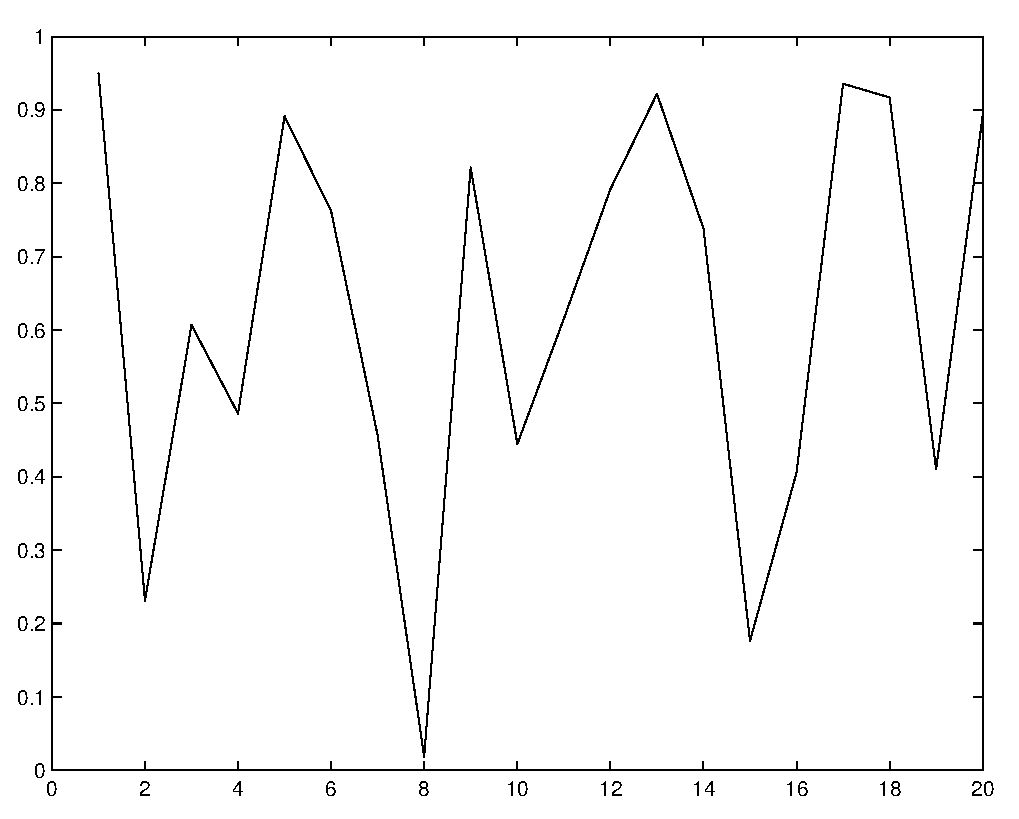
\epsfig{file=examplesofplota.eps,width=0.45\textwidth}} \quad
\subfigure[]{%
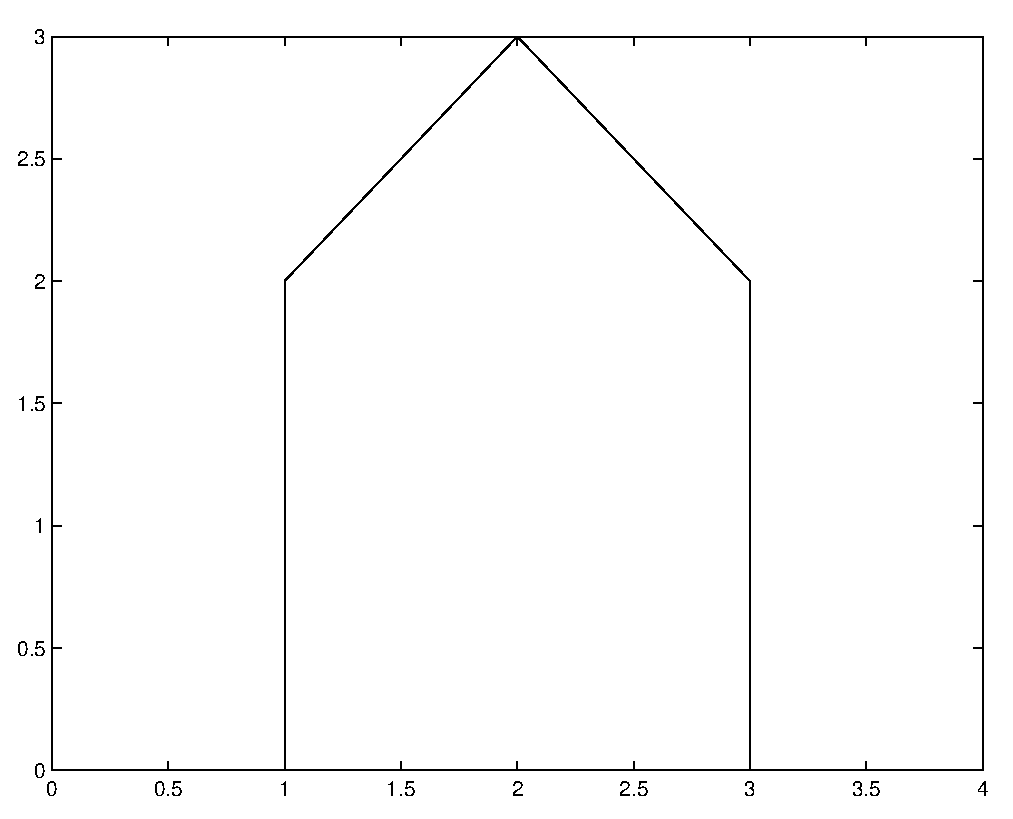
\epsfig{file=examplesofplotb.eps,width=0.45\textwidth}}} \quad
\caption{{\tt plot} 명령의 예} \label{plot}
\end{figure}

2-D graph is drawn using the {\tt plot} function. In the simplest form, one can display graphs that has only one vector value like {\tt plot(y)}. In this case, the elements of {\tt y} are drawn in the order of index. In other words, {\tt plot(rand(1,20))} graphs 20 random numbers in the order of $1\sim20$, connects all the consecutive points in lines, and prints the picture on the screen just like picture~\ref{plot}(a). If {\tt y} was a matrix, each elements of columns are drawn in order, drawing as many as the number of columns of the matrix. The axis are adjusted with the maximum and minimum values of the data and printed on the screen.

\vv The typical form of {\tt plot} is {\tt plot(x,y)}. Here, {\tt x} and {\tt y} are vectors with same dimensions. Let us execute the following command. \matlabp\texttt{\textbf{x = 0:pi/40:4*pi;}} \matlabp\texttt{\textbf{plot(x, sin(x))}} \vn In this graph, the coordinate of {\tt i}-th point is $(\tt x_{i}, y_{i})$.

\vv A line is drawing using the coordinates of {\tt x} and {\tt y} vectors. For instance, to draw a line connecting $(0,1)$ and $(4,3)$, type \matlabp\texttt{\textbf{plot([0,4], [1,3])}} \vn Here, {\tt [0,4]} mean {\tt x} coordinates of two points, and {\tt [1,3]} represent  the associated {\tt y} coordinates.

\vn \textbf{Practice question:} Draw a line connecting the following each points: $(0,1), (4,3), (2,0), (5,-2)$ \vn \textbf{Practice question:} Draw a house similar to the picture~\ref{plot}(b).

\subsubsection{Label}
One can attach label to the graph using the following commands.

\begin{description}
\item[\tt gtext('text')] \hfil \par
After executing this command, when one moves the mouse on the graph window, a cross-shaped thing is shown on the graph and waits for mouse click. After choosing the location by moving the mouse, the sentence {\tt 'text'} pops up on the graph window upon clicking. 

\item[\tt text(x, y, 'text')] \hfil \par
Prints {\tt 'text'} on {\tt (x,y)} location on the graph window. If {\tt x} and {\tt y} are vectors, {\tt 'text'} is printed on each points.

\item[\tt title('text')] \hfil \par
Prints the title {\tt 'text} at the very top part of the graph window.

\item[\tt xlabel('text')] \hfil \par
Puts an explanation on the x-axis.

\item[\tt ylabel('text')] \hfil \par
Puts an explanation on the y-axis.
\end{description}

\subsubsection{Drawing Many Graphs on the Same Axis}
There are at least 3 ways to draw many graphs on the same axis. However, if the recent graph contains data with bigger range than the previous data, then the graph can be rescaled.
\begin{enumerate}
\item The easiest way is to the command {\tt hold}, which holds the current graph on the graphic window. The graphs that are drawn after that are overlapped until the {\tt hold} status is turned off. The command that turns off {\tt hold} is {\tt hold off}.

\item The second way is to use the {\tt plot} command the following way. \vv \texttt{\textbf{plot(x1, y1, x2, y2, x3, y3, $\ldots$)}} \vn The merit of this way is that each vector pair is represented with different color/line forms. 

\item The third way is using {\tt plot(x,y)}. Here, {\tt x} and {\tt y} are either both matrices or one is vector and the other is matrix. If one of them is matrix and the other vector, then the column or row that matches the vector is printed with different color/line form. The column or row is chosen to match the vector. In case of square matrix, the column is selected. If both {\tt x} and {\tt y} are matrices that have same dimensions, the column of {\tt x} is matched with the column of {\tt y} and printed. If {\tt x} is not predetermined (just like {\tt plot(y)}), then the column of {\tt y} is matched with the index of the row and then drawn.

\end{enumerate}

\subsubsection{Form of Line, Output Symbol, and Color}
The form of line and output symbol can be selected by adding sentences to the {\tt plot} command.

\begin{description}
\item[\tt plot(x,y, '--')] \hfil \par
{\tt y} is plotted in point-line with respect to {\tt x}.
\item[\tt plot(x,y, 'o')] \hfil \par
Instead of connecting each points with line, the points are displayed in circle.
\item[\tt plot(x,y, '--o')] \hfil \par
Each data is connected with point-line and the points are displayed in circle.
\item[\tt plot(x,y, '--m')] \hfil \par
Displays magenta colored point-line. \end{description} \vn For diverse usage, refer to {\tt help plot}.

\subsubsection{Axis Scale}
In Matlab, the axis are automatically adjusted when drawing the graph. One can use command \vv \texttt{\textbf{axis([xmin, xmax, ymin, ymax])}} \vn to adjust the axis. One can return to the default setting using \texttt{\textbf{axis('auto')}}. The next command \vv \texttt{\textbf{v = axis}} \vn adjusts the current axis scale to the vector {\tt v}. One can maintain the current axis scale using {\tt axis(axis)}. Then, executing {\tt hold}, the next graph is printed with the current scale.

\vv Let us draw the following circle. \matlabp\texttt{\textbf{x = 0:pi/40:2*pi;}} \matlabp\texttt{\textbf{plot(cos(x), sin(x))}} \vn However, the thing that is shown in the screen does not look like circle. Why? The default setting for the length of each axis in Matlab is different. The command {\tt axis('equal')} equalizes the visual scale of {\tt x} and {\tt y} on the screen so that the circle shape will be printed. Use {\tt axis('normal')} to turn off this setting. Use the command {\tt axis('on')} and {\tt axis('off')} to set/erase the axis marking.

\subsubsection{Drawing Many Axes Using Subplot}

\begin{figure}[]
\center 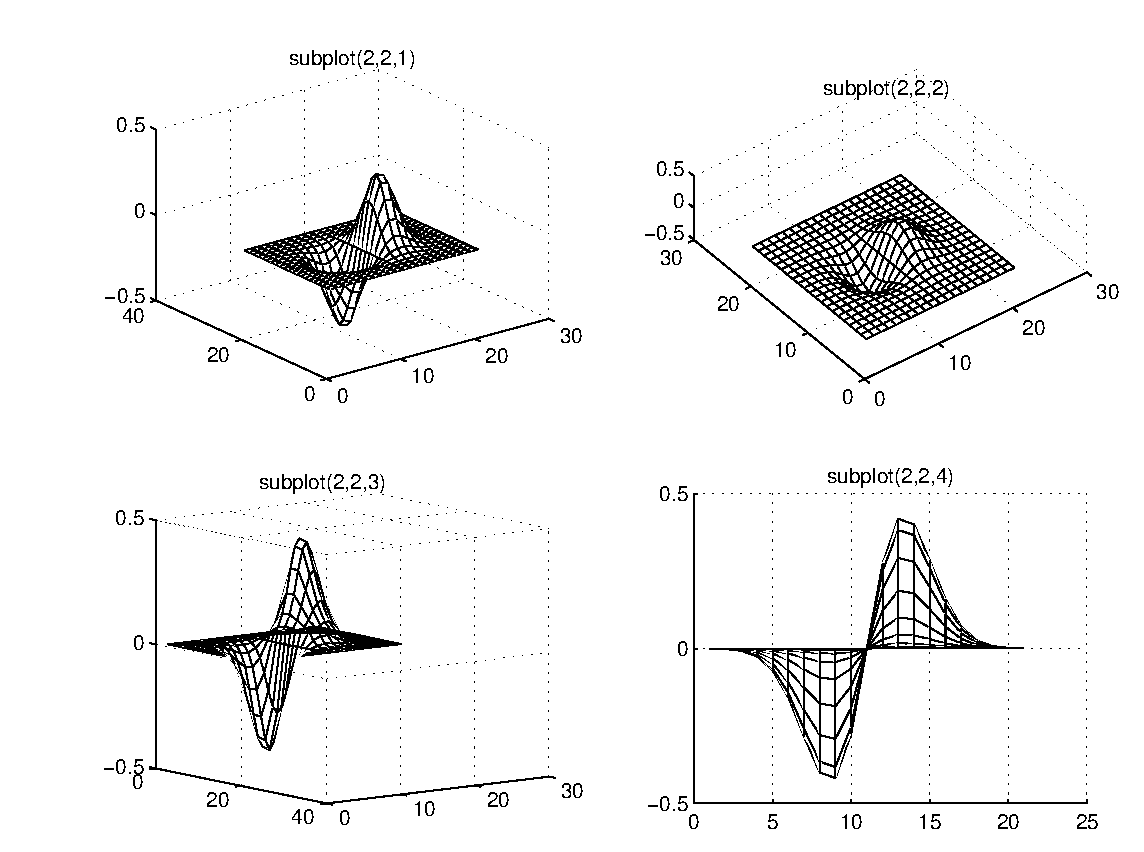
\epsfig{file=foursubplots.eps,%height=7cm ,
width=11cm, angle=0} \caption{\label{subplot}4개의 subplot:
3차원상에서 곡면의 회전}
\end{figure}

One can draw graphs with many different axes in one graphic window using {\tt subplot}. The command \texttt{\textbf{subplot(m, n, p)}} divides the current graphic window into $m \times n$ small axis, (starting from top left following the row) sets the {\tt p}-th graph as the current graph. For example, the following program makes four axes just like the picture~\ref{subplot}.

\begin{center}
\fbox{\parbox{10.5cm}{\begin{center}
\parbox{7.6cm}{\tt \% test\!$\_{}$subplot.m \\ \\
\tt [x,y] = meshgrid(-3:0.3:3, -3:0.3,3); \\
z = x.* exp(-x.\^{}2-y.\^{}2); \\
subplot(2,2,1) \\
mesh(z), title('subplot(2,2,1)') \\
subplot(2,2,2) \\
mesh(z) \\
view(-37.5, 70), title('subplot(2,2,2)') \\
subplot(2,2,3) \\
mesh(z) \\
view(-37.5, -10), title('subplot(2,2,3)') \\
subplot(2,2,4) \\
mesh(z) \\
view(0,0), title('subplot(2,2,4)')}  \end{center} }}
\end{center}
\vn The command {\tt subplot(1,1,1)} sets the graphic axis back to one.

\subsubsection{figure, clf, cla}
Command {\tt figure} produces a new figure window. \par

\begin{description}
\item[{\tt figure(N)}] \hfil\par
Produces {\tt N}-th figure window. Commands related to graphic after this will be executed in this window.
\item[{\tt clf}] \hfil\par
Everything except the window of the current figure window will be deleted. Thus, the properties of the current window will also be deleted.
\item[{\tt cla}] \hfil\par
Deletets all the lines, symbols, texts except the axis and axis markings in the current figure window.
\end{description}

\subsubsection{Inputs related to graphics}
The command \vv \texttt{\textbf{[x, y] = ginput}} \vn saves all the points that are inputted by the mouse on the current window. Cross shape is shown on the screen, and saves the points the mouse clicks. {\tt Enter} finishes this command. The command \vv \texttt{\textbf{[x, y] = ginput(n)}} \vn is exactly the same as {\tt ginput} except it only saves {\tt n} points. Use {\tt help} or {\tt doc} to earn more information..

\subsubsection{Logarithmic plot}

\begin{figure}[]
\center 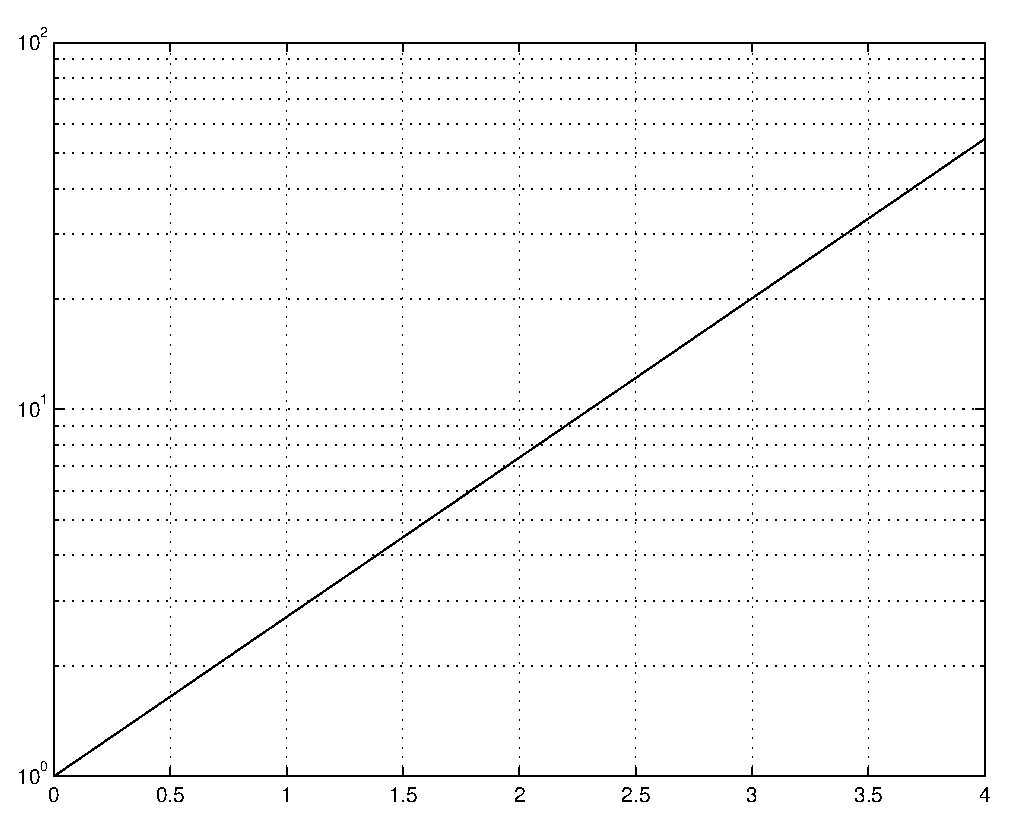
\epsfig{file=logarithmicplot.eps, height=7cm, %width=10cm,
angle=0} \caption{\label{log}Logarithmic plot}
\end{figure}

Command \texttt{\textbf{semilogy(x, y)}} displays the graph {\tt y} with $\log_{10}$ scale and {\tt x} with linear scale. For instance, \matlabp\texttt{\textbf{x = 0:0.01:4;}} \matlabp\texttt{\textbf{semilogy(x, exp(x)), grid}} \vn draws the graph like picture~\ref{log}. The increase of equidistant interval of {\tt y}-axis is expressed in exponent of 10. In addition, the marking in the {\tt y}-axis are drawn to show 1, 2, 3, $\ldots$, 10, 20, 30, $\ldots$, 100, $\ldots$ starting from bottom. There are also similar commands like {\tt semilogx} and {\tt loglog}. {\tt x} and {\tt y} can be vector or matrix just like they were with {\tt plot}.

\vn \textbf{Practice question:} Draw graph of $x^{2}, x^{3}, x^{4}, \exp{x^{2}}$ with $ 0\leq x \leq 10$ using {\tt semilogy}.

\subsubsection{Polar Coordinate} 

\begin{figure}[]
\center 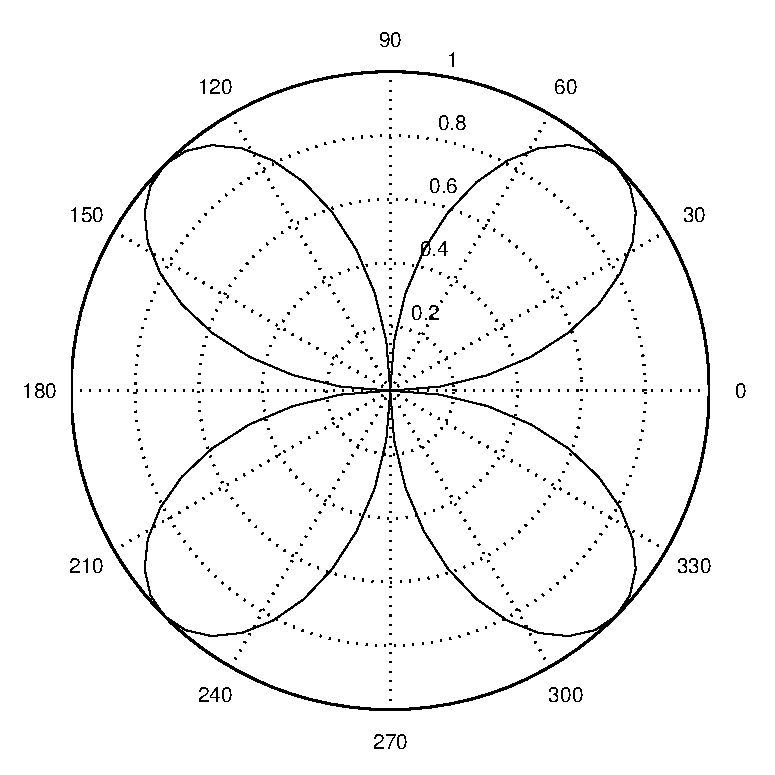
\epsfig{file=polarplot.eps,height=7cm, %width=10cm,
angle=0} \caption{Polar plot: $r=\sin 2\theta$ } \label{polar}
\end{figure}

The command \texttt{\textbf{polar(theta, r)}} uses angle $\theta$ and size $r$ to show the position of the point. For instance, \matlabp\texttt{\textbf{x = 0:pi/40:2*pi;}} \matlabp\texttt{\textbf{polar(x, sin(2*x)), grid}} \vn produces graph like picture~\ref{polar}.

\subsubsection{Drawing a Graph of a Function that Changes Quickly}

\begin{figure}
\centering
\mbox{%
\subfigure[]{%
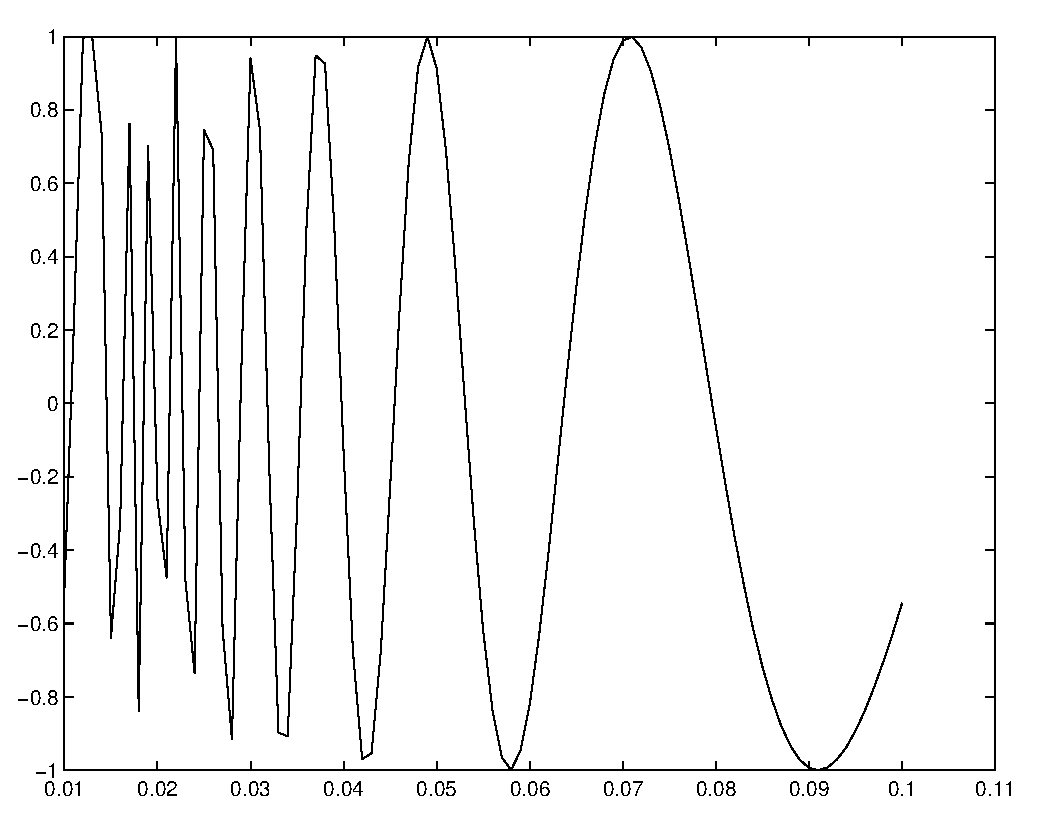
\epsfig{file=ysina.eps,width=0.45\textwidth}} \quad
\subfigure[]{%
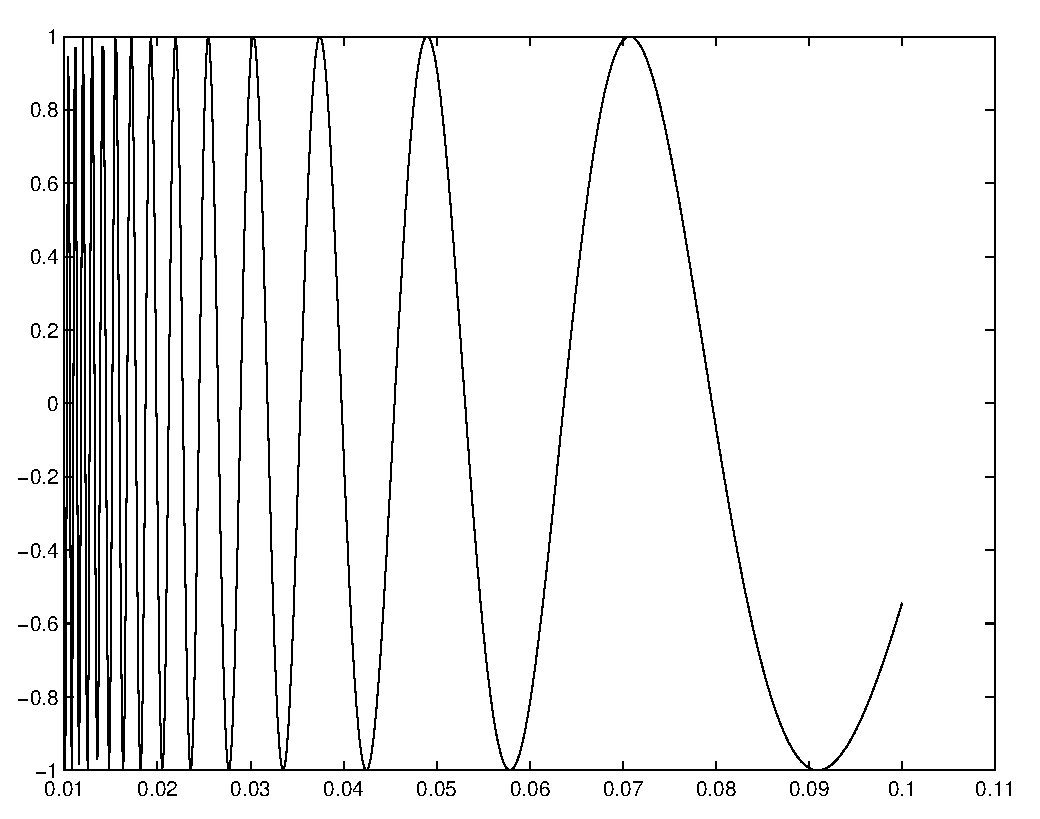
\epsfig{file=ysinb.eps,width=0.45\textwidth}}} \caption{$y
=\sin(1/x)$} \label{sin}
\end{figure}

Until now, the graphs were drawn with data that has $x$-axis all distributed equally, like the example \texttt{\textbf{x = 0:0.01:4}}. If a function to be drawn rapidly changes in a certain domain, then the distribution of $x$-axis will be inefficient, and the graph will not be drawn properly. For instance, \matlabp\texttt{\textbf{x = 0.01:0.001:0.1;}} \matlabp\texttt{\textbf{plot(x, sin(1./x))}} \vn will draw the graph like picture~\ref{sin}(a). However, if the increment of $x$ is reduced to 0.0001, then the graph like picture~\ref{sin}(b) will be drawn. The two graphs are clearly different in the domain $x < 0.04$.

\vv Matlab provides {\tt fplot}, which is a more efficient function. When it comes to drawing a function like $\sin(1/x)$, {\tt fplot} calculates rapid changing places more frequently. However, the command {\tt fplot} has a demerit, which is it must use function file.

\subsubsection{Many Commands related to 2 Dimensional Graphs}
Matlab provides many commands that express functions into graphs. Here, we state some examples, but we wish for the reader to use {\tt help} or {\tt doc} to get more detailed information.

\begin{description}
\item[\tt bar] \hfil\par Draws bar graph. \item[\tt compass] \hfil\par Displays the vector with entries size and direction of complex number with an arrow starting from the origin.
\item[\tt errorbar] \hfil\par Displays error bar. \item[\tt hist] \hfil\par Draws histogram. \item[\tt quiver] \hfil\par Draws many different types of vector fields(for instance, gradient) using little arrows.
\item[\tt fill] \hfil\par Draws polygon and fills in with given color.
\end{description}

\subsection{3 Dimensional Graph}
Matlab provides many functions that can express 3 dimensional graphs. This susbsection will be a brief introduction to these functions.

\subsubsection{Plot3}

\begin{figure}
\centering
\mbox{%
\subfigure[]{%
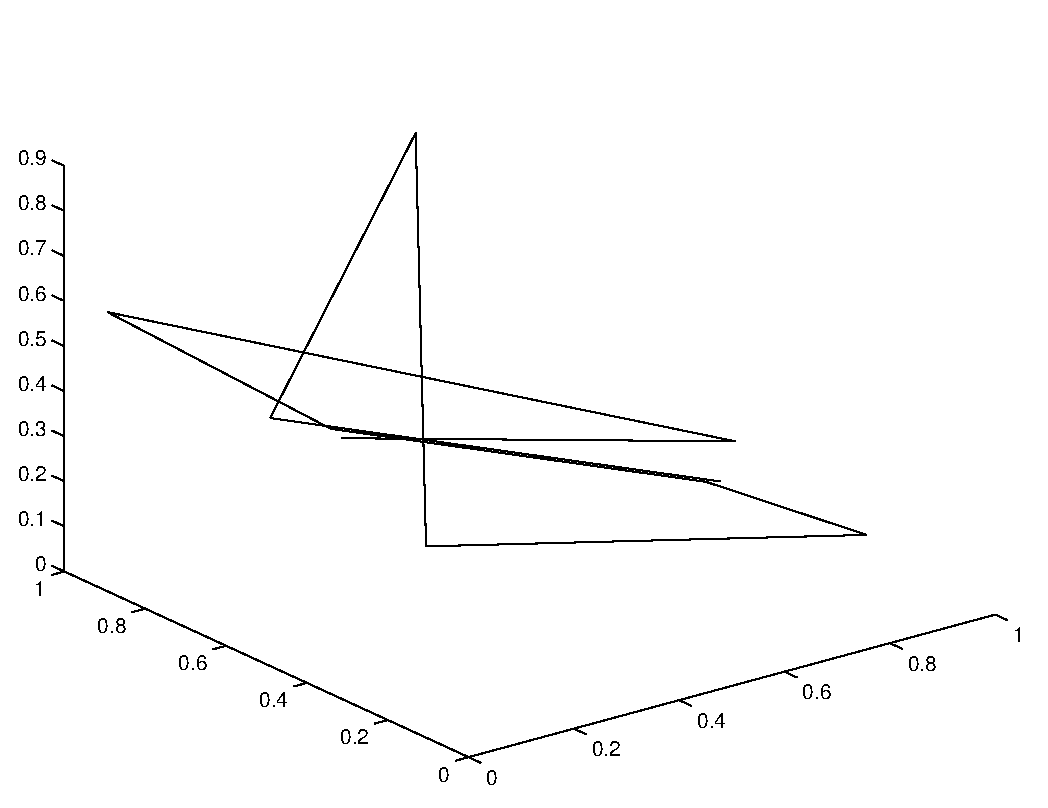
\epsfig{file=plot3a.eps,width=0.45\textwidth}} \quad
\subfigure[]{%
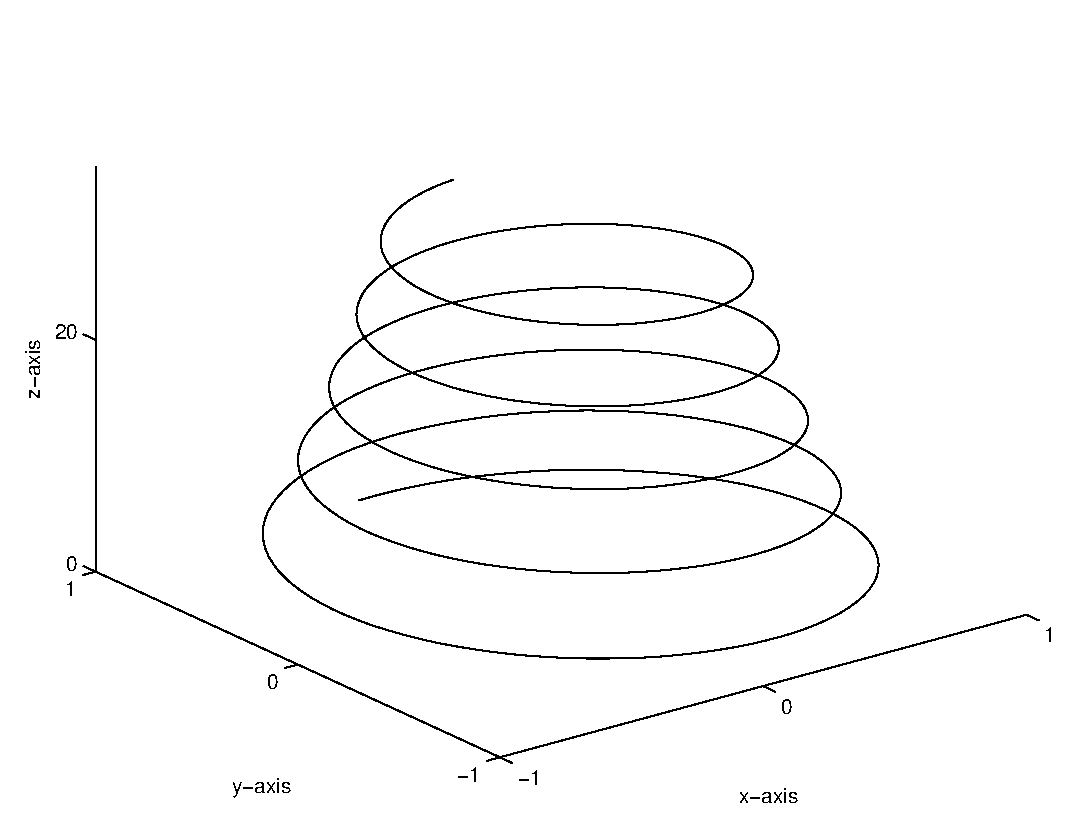
\epsfig{file=exampleofplot3b.eps,width=0.45\textwidth}}} \quad
\caption{example of command plot3}\label{plot3}
\end{figure}

The command {\tt plot3} is a 3 dimensional version of {\tt plot}, and if we write \matlabp\texttt{\textbf{plot3(x, y, z)}} \vn then a line connecting the points $(x_i, y_i, z_i)$ will be drawn in 3 dimension. For instance, \matlabp\texttt{\textbf{plot3(rand(1,10), rand(1,10), rand(1,10))}} \vn uses 10 random points to draw a line in 3 dimension, like picture~\ref{plot3}(a). And another example, \matlabp\texttt{\textbf{t = 0:pi/50:10*pi;}} \matlabp\texttt{\textbf{plot3(exp(-0.02*t).*sin(t), exp(-0.02*t).*cos(t), t), \ldots}} \par\texttt{\textbf{xlabel('x-axis'), ylabel('y-axis'), zlabel('z-axis') }}\vn draws a dwindling spiral like picture~\ref{plot3}(b). Be careful on the direction of $x$-axis, $y$-axis, $z$-axis, and pay attention to the fact that label was marked for each axis.

\subsubsection{Mesh Surface}
The following is an example regarding mesh surface.

\begin{center}
\fbox{\parbox{10.5cm}{\begin{center}
\parbox{8.4cm}{\tt \% Mexican\!$\_{}$hat.m \\ \\
\tt [x y] = meshgrid(-7.5:0.5:7.5, -7.5:0.5:7.5);  \\
r = sqrt(x.\^{}2 + y.\^{}2) + eps; \\
z = sin(r)./r; \\
mesh(z);}  \end{center} }}
\end{center}

\vv To know how these surfaces are drawn, let us study a simple example like $z = x^{2} - y^{2}$. We want a graph that shows the change in $z$ value when there is a change in values in $x$-$y$ plane. Let us think only in the domain $0 \leq x \leq 5, 0 \leq y \leq 5$ for this example. First use Matlab command {\tt meshgrid} to produce grid on the $x$-$y$ plane where the surface will be drawn. \matlabp\texttt{\textbf{[x y] = meshgrid(0:5, 0:5)}} \vn This command produces two matrices {\tt x, y} like the following.
$$\begin{array}{ccccccc}
{\tt x =} & & & & & & \\
& 0 & 1 & 2 & 3 & 4 & 5 \\
& 0 & 1 & 2 & 3 & 4 & 5 \\
& 0 & 1 & 2 & 3 & 4 & 5 \\
& 0 & 1 & 2 & 3 & 4 & 5 \\
& 0 & 1 & 2 & 3 & 4 & 5 \\
& 0 & 1 & 2 & 3 & 4 & 5
      \end{array}\qquad\qquad
\begin{array}{ccccccc}
{\tt y =} & & & & & & \\
& 0 & 0 & 0 & 0 & 0 & 0 \\
& 1 & 1 & 1 & 1 & 1 & 1 \\
& 2 & 2 & 2 & 2 & 2 & 2 \\
& 3 & 3 & 3 & 3 & 3 & 3 \\
& 4 & 4 & 4 & 4 & 4 & 4 \\
& 5 & 5 & 5 & 5 & 5 & 5
\end{array}$$

\vn As we can see from above, matrix {\tt x} represents each grid of $x$-axis, and matrix {\tt y} represents each grid of $y$-axis. If the grid of $x$-direction and that of $y$-direction are of same shape, then we can write in the following short form. \matlabp\texttt{\textbf{[x y] = meshgrid(0:5)}} \vn And as can be predicted with the Matlab matrix operation, the command \texttt{\textbf{z = x.\^{}2-y.\^{}2}} produces the following matrix.
$$\begin{array}{rrrrrrr}
{\tt z =} & & & & & & \\
& 0  &  1  &  4  &  9  &  16  &  25 \\
& -1  &  0  &  3  &  8  &  15  &  24 \\
& -4  &  -3  &  0  &  5  &  12  &  21 \\
& -9  &  -8  &  -5  &  0  &  7  &  16 \\
& -16  &  -15  &  -12  &  -7  &  0  &  9 \\
& -25  &  -24  &  -21  &  -16  &  -9  &  0
\end{array}$$

\vn For instance, at the point $(5, 2)$, z takes the value $5^{2}-2^{2} = 21$. Fortunately, one does not need to be concerned with the precise relationship between the coordinate system of the grid and the index of the matrix. This is automatically adjusted by {\tt meshgrid}.

\begin{figure}[]
\center 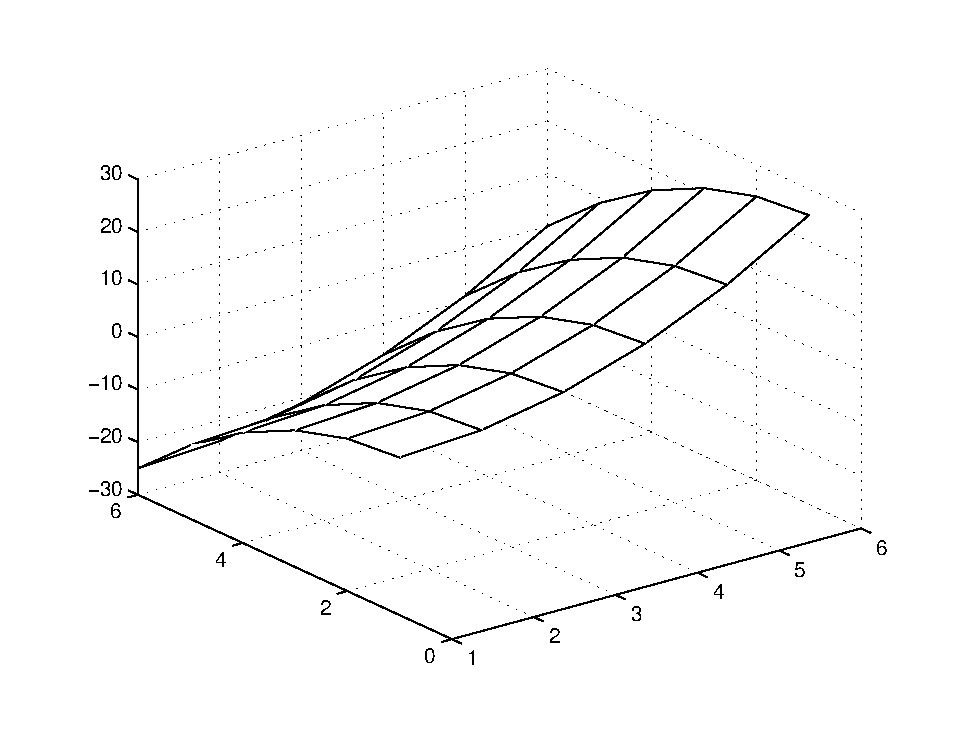
\epsfig{file=surface.eps, %fig7surf.eps,
height=7cm,%width=10cm,
angle=0} \caption{curved surface $z = x^{2}-y^{2}$} \label{surf}
\end{figure}

\vv The command {\tt mesh(z)} produces graph with lattice-like surface, where the points on the grid are raised to the surface and then connected to form the lattice. In other words, {\tt mesh} draws a `wire mesh'-like surface. If one does not want color, then one can type \matlabp{\tt mesh(z,'EdgeColor','black')} \vn In addition, another command {\tt surf} draws a lattice-like surface composed of small colored tiles. Use {\tt help} or {\tt doc} to learn more about {\tt mesh} and {\tt surf}.

If one is using Matlab student edition, then one must know that there is a limit to grid size when using {\tt meshgrid}. The limit is that the size of the row or column of matrix must be at most 32, and the size of matrix must not exceed 8192.

\vn \textbf{Practice question:} Use the command  \vv \texttt{\textbf{[x y] = meshgrid(0:0.25:5);}} \vn to draw a denser mesh than picture~\ref{surf}.

\vn \textbf{Practice question:} The distribution of temperature on the iron plate is as follows.
$$u(x, y) = 80 y^{2} e^{-x^{2}-0.3y^{2}}$$ \noindent With the domain $-2.1 \leq x \leq 2.1, -6 \leq y \leq 6$, draw the curved surface $u$ with the grid size of each direction as 0.15.

\subsubsection{Drawing Contour}
\begin{figure}
\centering
\mbox{%
\subfigure[]{%
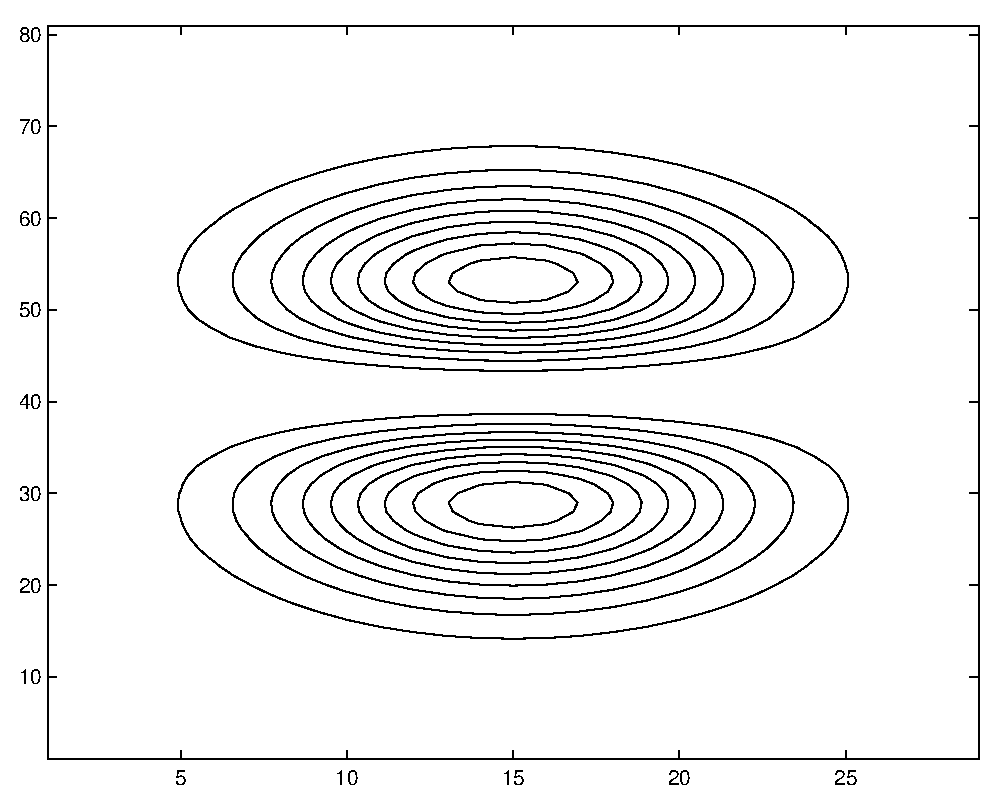
\epsfig{file=contoura.eps,width=0.45\textwidth}} \quad
\subfigure[]{%
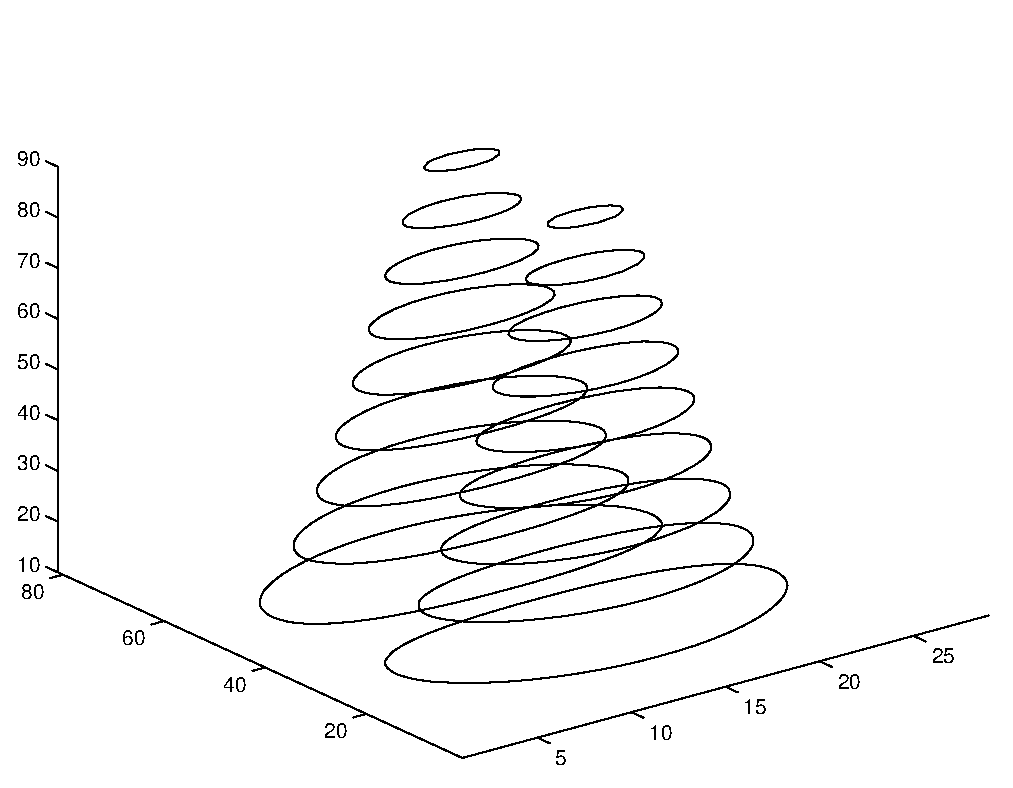
\epsfig{file=contour3b.eps,width=0.45\textwidth}}} \caption{Contour
plot} \label{contour}
\end{figure}

After solving the practice questions above, execute the following command. \matlabp\texttt{\textbf{ contour(u)}} \vn Then, one can earn a contour(isothermal line) about the distribution of temperature like picture~\ref{contour}(a). The command {\tt contour} can take second input variable. For this second variable, one inputs how many lines the contour will draw or a vector with specific values for drawing contour. Use command {\tt contour3} to draw a 3 dimensional contour like picture~\ref{contour}(b). One can make contour label with the command {\tt clabel}.

\begin{figure}
\centering
\mbox{%
\subfigure[]{%
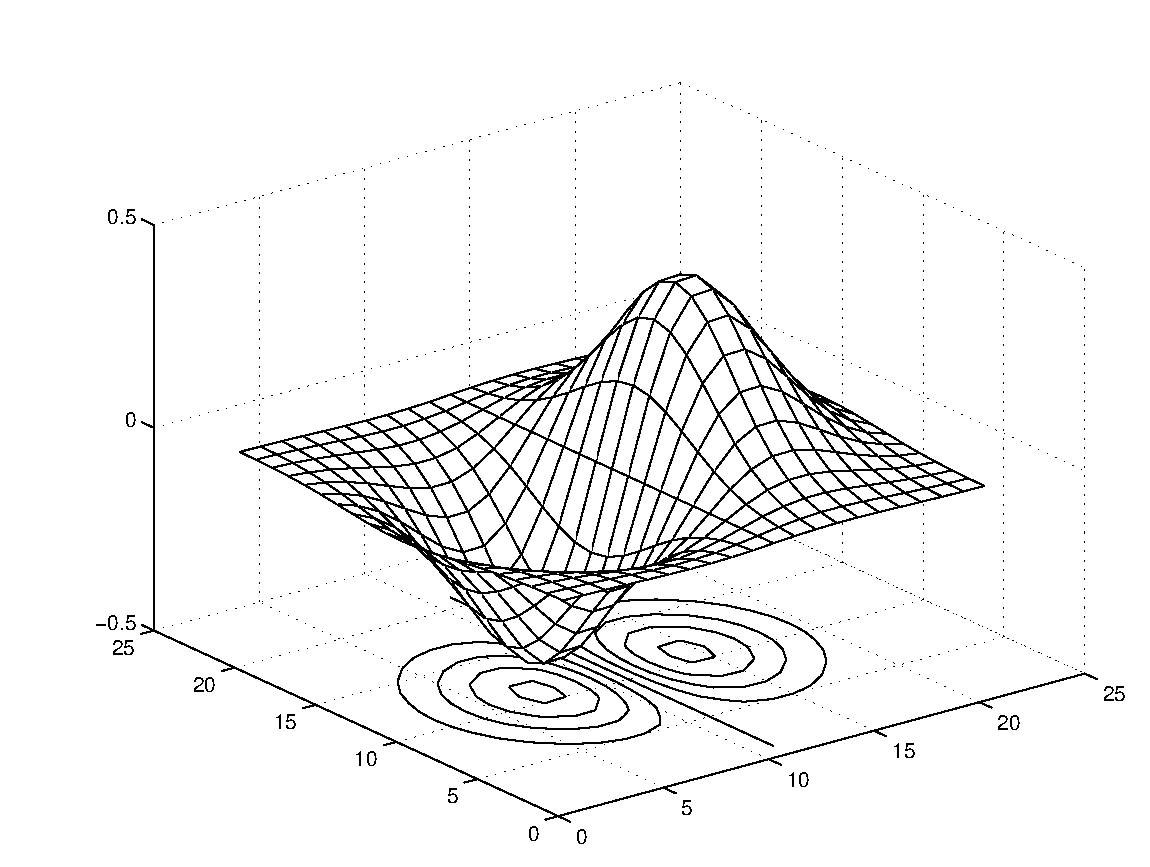
\epsfig{file=fig710a.eps,width=0.45\textwidth}} \quad
\subfigure[]{%
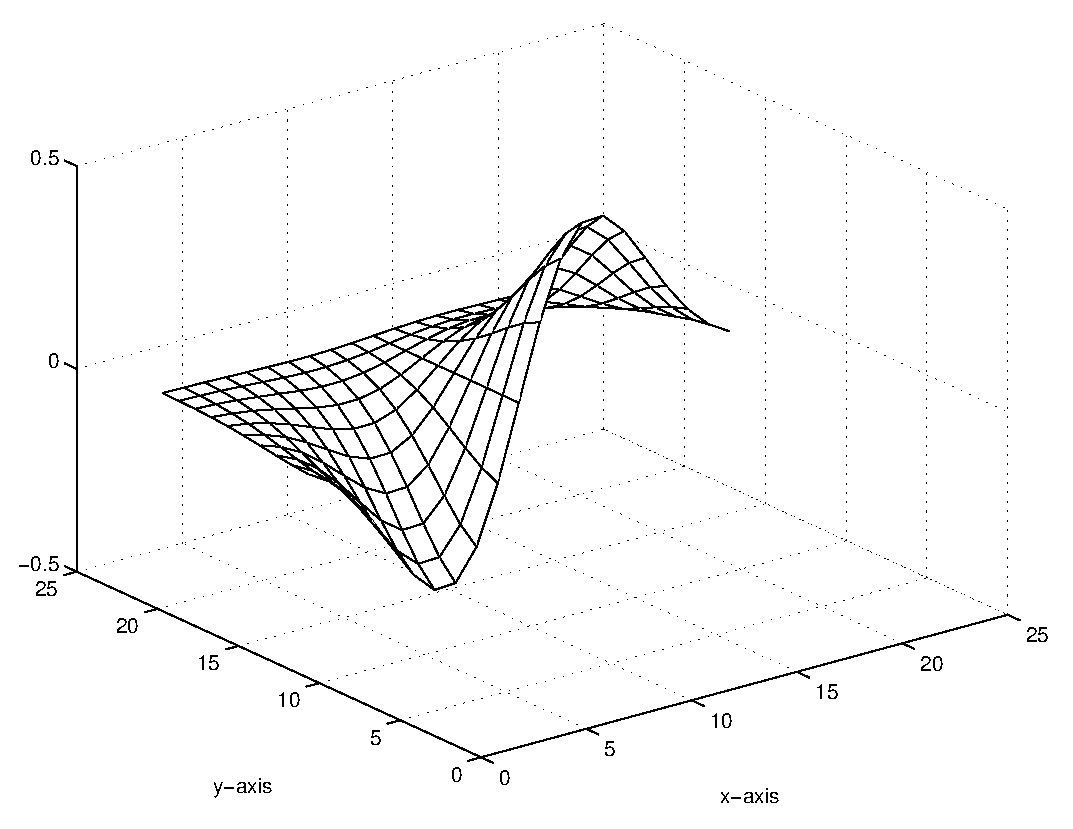
\epsfig{file=fig710b.eps,width=0.45\textwidth}}} \caption{(a)
meshc \quad (b) Erasing part of curved surface} \label{meshc}
\end{figure}

\vv To display both contour and mesh together, one can use {\tt meshc} or {\tt surfc}. For instance, the following program \matlabp\texttt{\textbf{[x y] = meshgrid(-2:0.2:2); }} \matlabp\texttt{\textbf{ z = x.*exp(-x.\^{}2 - y.\^{}2); }} \matlabp\texttt{\textbf{meshc(z);}} \vn draws a graph like picture~\ref{meshc}(a).

\subsubsection{Deletion of Curved Surface Due to NaN(Not a Number)}
If the matrix that holds information on the curved surface contains NaN, then this value does not appear in the graph, and because of this, a part of the curved surface will be omitted. Let us study the following example.

\begin{center}
\fbox{\parbox{10.5cm}{\begin{center}
\parbox{8.0cm}{\tt \% cropping.m \\ \\
\tt [x y] = meshgrid(-2:.2:2);  \\
z = x.*exp(-x.\^{}2 - y.\^{}2); \\
c = z;\qquad \% preserve the original surface \\
c(1:11, 1:21) = nan; \\
mesh(c), xlabel(`x-axis'), ylabel(`y-axis')}  \end{center} }}
\end{center}
\vn The above program will display the graph like picture~\ref{meshc}(b).

\subsubsection{quiver}
The command {\tt quiver} draws a vector that starts at 2 dimensional point. Although it is drawn in 2 dimensional graph, it is occasionally used with {\tt contour}, which helps understanding changes in 3 dimensional curved surfaces. For instance, let us think about $V = x^{2} + y$, which is a scalar function with 2 variables for input. The gradient of V is defined as the following vector field.
\begin{eqnarray*}
\nabla V & = & \left(\frac{\partial V}{\partial x}, \frac{\partial
V}{\partial y}\right) \\
         & = & (2x, 1)
\end{eqnarray*}

\begin{figure}[]
\center 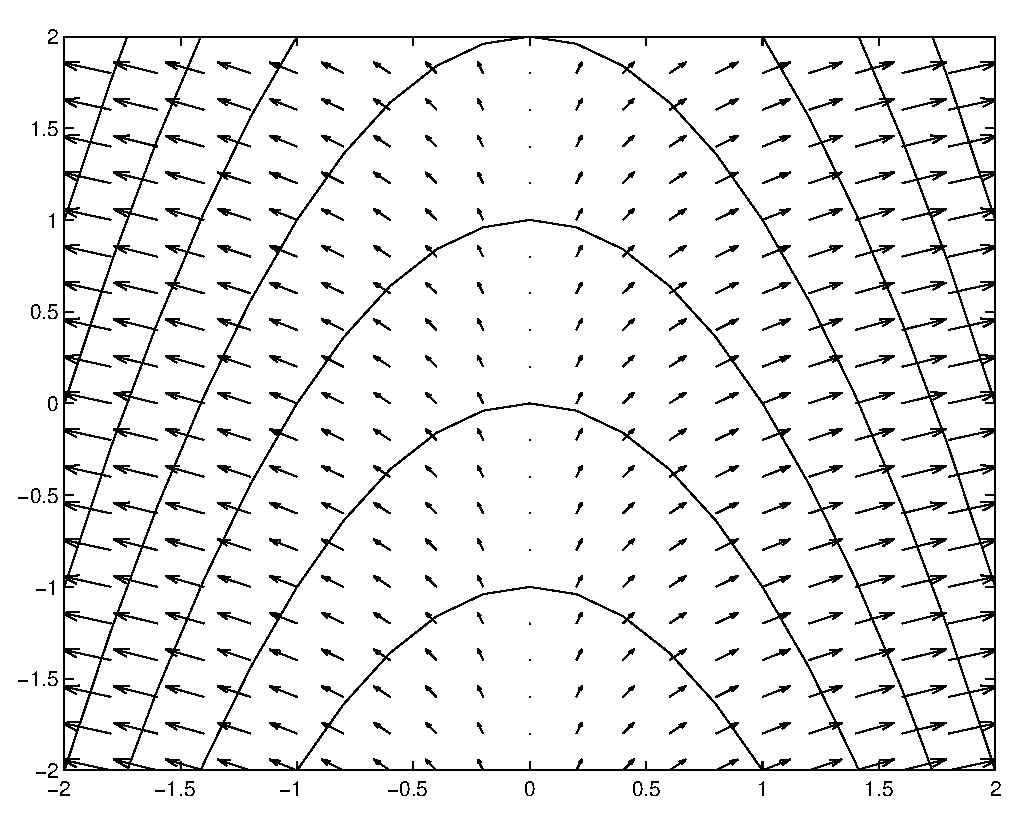
\epsfig{file=fig711.eps,height=7cm, %width=10cm,
angle=0} \caption{Gradient and contour} \label{grad}
\end{figure}

\noindent The following program draws the direction of $\nabla V$ for each points in $x$-$y$ plane(refer to picture~\ref{grad}).

\begin{center}
\fbox{\parbox{10.5cm}{\begin{center}
\parbox{5.6cm}{\tt \% test\!$\_{}$quiver.m \\ \\
\tt [x y] = meshgrid(-2:.2:2);  \\
V = x.\^{}2 + y; \\
dx = 2*x; \\
dy = ones(size(y)); \\
axis equal \\
contour(x, y, V), hold on \\
quiver(x, y, dx, dy), hold off}  \end{center} }}
\end{center}

`Contour' is a series of {\tt level surface}. Gradient of a random point is perpendicular to the level surface that passes through that point. When drawing a contour, the vectors {\tt x} and {\tt y} are required for labeling the axes. What will happen if take this out and just use {\tt contour(V)} and execute the above {\tt test\!$\_{}$quiver.m}? Let us try to predict the result before we execute it.

Another option regarding {\tt quiver} is that one can change the size of the arrows. See {\tt help} or {\tt doc}.

If it is not possible to differentiate the vector $V$ or if one does not wish to differentiate it, then one can use the command {\tt gradient} to calculate the derivative.
\matlabp\texttt{\textbf{[dx dy] = gradient(V, 0.2, 0.2);}} \vn 0.2 means the increment with respect to $x$ and $y$ directions for approximate calculation.

\subsubsection{Pseudocolor}
The following program  \matlabp\texttt{\textbf{[x, y] = meshgrid(-2:.2:2); }} \matlabp\texttt{\textbf{z = x.*exp(-x.\^{}2 - y.\^{}2); }} \matlabp\texttt{\textbf{pcolor(z), shading flat, colormap(hot) }} \vn draws a contour that expresses height using mixture of red, orange, and yellow. The command {\tt shading flat} eliminates the grid line. {\tt pcolor} means pseudocolor. Each element of the matrix {\tt z} is used as index of color map(in this case hot) that determines the color which will express the element. If one wants a cool color, then try {\tt colormap(cool)}.\^{}\^{} Does it feel cool? There is yet another color map, {\tt colormap(hsv)}, where {\tt hsv} stands for huge-saturation-value.

\subsubsection{Visualization of matrix}

\begin{figure}[]
\center 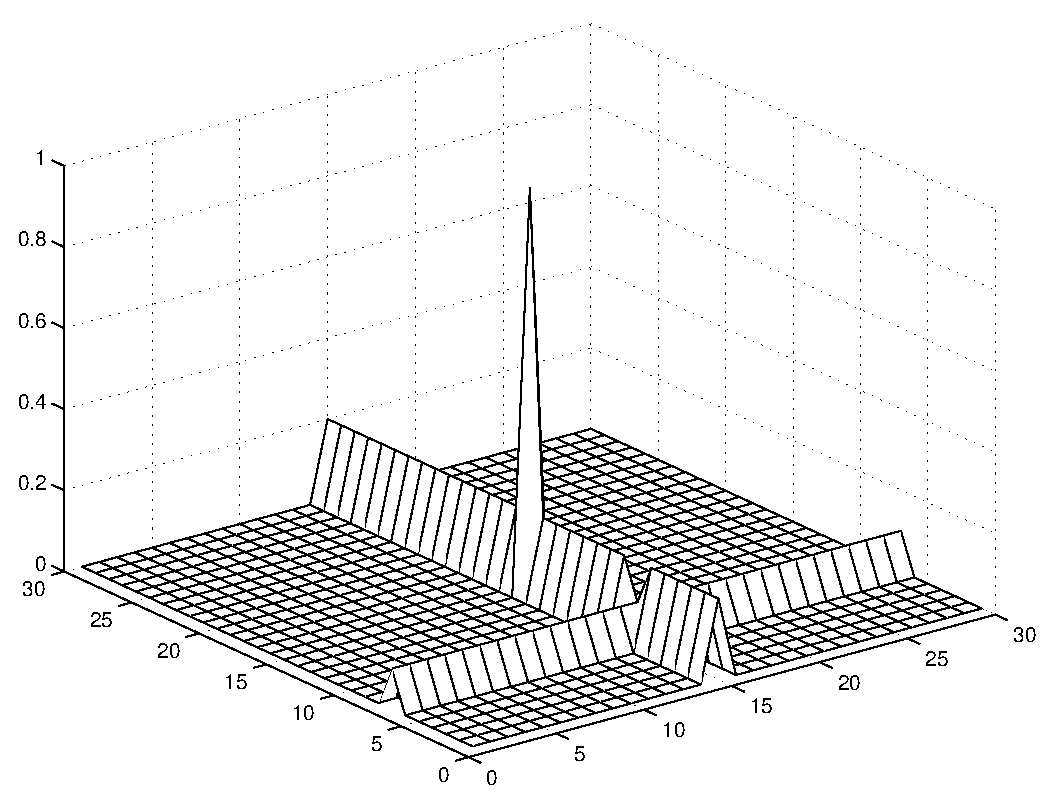
\epsfig{file=viewmat.eps,height=7cm,%width=10cm,
angle=0} \caption{visualization of matrix} \label{mat}
\end{figure}

The command {\tt mesh} can `visualize' the matrix. The following program displays the graph like picture~\ref{mat}.

\begin{center}
\fbox{\parbox{10.5cm}{\begin{center}
\parbox{4.7cm}{\tt \% visual\!$\_{}$mat.m \\ \\
\tt a = zeros(30);  \\
a(:,15) = 0.2*ones(30,1); \\
a(7,:) = 0.1*ones(1,30); \\
a(15,15) = 1; \\
mesh(a)}  \end{center} }}
\end{center}
\vn The size of the matrix {\tt a} is $30 \times 30$. The middle element {\tt a(15,15)} is 1, and every element of the 7-th row is 0.1, and the remaining elements of the 15-th row is 0.2. {\tt mesh(a)} cognizes every rows and columns of matrix a as coordinates of $x$-$y$. In other words, the value of {\tt a(i,j)} is the height of the curved surface mesh at point {\tt (i,j)}.

\subsubsection{Rotating 3 Dimensional Graph}
{\tt view} is a command which designates observation point when viewing a 3 dimensional graph. To see how this works, let us execute the following program which rotates the visualized matrix picture~\ref{mat}.

\begin{center}
\fbox{\parbox{10.5cm}{\begin{center}
\parbox{5cm}{\tt \% rotation.m \\ \\
\tt a = zeros(30);  \\
a(:,15) = 0.2*ones(30,1); \\
a(7,:) = 0.1*ones(1,30); \\
a(15,15) = 1; \\
el = 30; \\
for az = -37.5:15:-37.5+360 \\
\phantom{for}mesh(a), view(az, el) \\
\phantom{for}pause(0.5) \\
end}  \end{center} }}
\end{center}
\vn The command {\tt view} requires two angles. The first, as can be seen in the example, is azimuth {\tt az} on the $x$-$y$ plane that has degree as its unit. {\tt az} rotates the observation point about $z$-axis - in other words, the 'sharp point' at $(15,15)$ in picture~\ref{mat} - counterclockwise. The default value for {\tt az} is $-37.5^{\circ}$. Therefore, the above program rotates the observation point about $z$-axis $15^{\circ}$ each time from the default value. The second angle of {\tt view} is {\tt el} which expresses altitude with degree as its unit. This means the angle between the $z$-axis and $x$-$y$ plane. For instance, $90^{\circ}$ represents 2 dimensional graphic, in other words, looking down from above. If the value of altitude is positive, then the observer is above the $x$-$y$ plane, and if negative, then is below the plane. The default value is $30^{\circ}$.

\vv The command {\tt pause(n)} stops the execution for {\tt n} seconds.

\vn \textbf{Practice question:} Fix the above program so that the value of {\tt az} is fixed as the default value and and the value of {\tt el} is gradually changing.

\subsubsection{Lighting}
One can materialize lighting and shadow effect using the command {\tt surfl}. Try the following.

\matlabp\texttt{\textbf{[x, y] = meshgrid(-2:0.05:2);}}
\matlabp\texttt{\textbf{z = x.*exp(-x.\^{}2 - y.\^{}2); }}
\matlabp\texttt{\textbf{surfl(z, [-20 50]), colormap(gray),
shading flat}} \vn The location of the source of light is determined by the second variable of {\tt surfl}, with the first value being azimuth and the second being altitude. To make a natural reflection light, one must set the grid compact so that the grid is not visualizable. (In this case, $81\times 81$)
%% section 1
\chapter {MATLAB Basics}
% section 2
\chapter {Systems of Linear Equations}

%\section{Introduction to Systems of Linear Equations}
%\section{Solving Linear Systems by Row Reduction}

\section{Introduction to Systems of Linear Equatios}

No MATLAB problems in this section.

\section{Solving Linear Ssytems by Row Reduction}
\begin{exer}
(\textit{Reduced Row Echelon Form with Pivot Columns and Ranks}) \\
In MATLAB, there are several useful commands for matrices such as \textit{rref} command which produces the reduced row echelon form together with the pivot columns, and \textit{rank} command which gives the number of the leading $1$'s without finding its row echelon form. Find the reduced row echelon form, the pivot columns, and the rank of the matrix $A$, where
\vspace{2mm}
\begin{displaymath}
A = \left[\begin{array}{rrrrr} 2& \hspace{1mm}-3& \hspace{1mm} 1& \hspace{3mm} 0& \hspace{2mm} 4 \\ 1 & 1 & 2 & 2 & 0 \\ 3 & 0 & -1 & 4 & 5 \\ 1 & 6 & 5 & 6 & -4 \end{array} \right].
\end{displaymath}
\end{exer}

\begin{sol}

\begin{verbatim}

% Construct the matrix A.
A=[2 -3 1 0 4; 1 1 2 2 0; 3 0 -1 4 5; 1 6 5 6 -4]; 

% Display the format of each entry as a rational form
format rat; 

% Find the reduced row echelon form 
% and the pivot columns of the matrix A.
[rref_A pivotcols] = rref(A);

% Find the rank of the matrix A.
rank_A = rank(A); 

disp('The reduced row echelon form is'); disp(rref_A);
disp('The pivot columns are'); disp(pivotcols);
disp('The number of the leading 1 is'); disp(rank_A);
\end{verbatim}

\begin{outputs}

\begin{verbatim}

The reduced row echelon form is
       1    0    0   17/13   3/2
       0    1    0   11/13  -1/2
       0    0    1   -1/13  -1/2
       0    0    0      0     0

The pivot columns are
       1    2    3

The number of leading 1 is
       3
\end{verbatim}
\end{outputs}
\end{sol}


\vspace{5mm}
\begin{exer}
(\textit{Linear Combinations}) Use the MATLAB command \textit{rref} to express the vector $\mathbf{b}=(-21, \hspace{1mm}-60, \hspace{1mm}-3, \hspace{1mm}108, \hspace{1mm}84)$ as a linear combination of $\mathbf{v_{1}}$, $\mathbf{v_{2}}$, and $\mathbf{v_{3}}$ where 
$\mathbf{v_{1}}=(1, \hspace{1mm} -1, \hspace{1mm}3, \hspace{1mm}11, \hspace{1mm}20)$, 
$\mathbf{v_{2}}=(10, \hspace{1mm}5, \hspace{1mm}15, \hspace{1mm}20, \hspace{1mm}11)$, 
and 
$\mathbf{v_{3}}=(3, \hspace{1mm}3, \hspace{1mm}4, \hspace{1mm}4, \hspace{1mm}9)$.
\end{exer}

\begin{sol}
\begin{verbatim}

% Construct b as a column vector.
b = [-21 -60 -3 108 84]';
% Set v1, v2, v3 as column vectors. 
v1 = [1 -1 3 11 20]'; 
v2 = [10 5 15 20 11]'; 
v3 = [3 3 4 4 9]';
% Set a matrix A with column vectors v1, v2 and v3. 
A = [v1 v2 v3]; 
% Augmented matrix [A | b].
augA = [A b]; 
% Reduced row echelon form of augA.
rref_augA = rref(augA);
% Solution vector from rref_augA. 
x = rref_augA(1:3, 4); 

% Display the result as an integer form.
format rat; 
disp('b is a linear combination of x(1)*v1+x(2)*v2+x(3)*v3, where');
disp('x(1) ='); disp(x(1)); disp('x(2) ='); disp(x(2));
disp('x(3) ='); disp(x(3));
\end{verbatim}

\begin{outputs}

\begin{verbatim}

b is a linear combination of x(1)*v1+x(2)*v2+x(3)*v3, where
x(1) =
      12

x(2) =
       3

x(3) =
     -21
\end{verbatim}
\end{outputs}
\end{sol}
% section3
\chapter {Matrices and Matrix Algebra}

\section{Operations on Matrices}

No MATLAB problems in this section.


\section{Inverses; Algebraic Properties of Matrices}

\begin{exer}
In this problem, we compute $A^{5} - 3A^{3} + 7A - 4I$ for the matrix $A$, where
$$
A = \left[\begin{array}{rrrr} 1&\hspace{3mm} 2&\hspace{1mm} -3&\hspace{2mm} 0\\ 1 & 1 & -2 & 1 \\ 2 & 1 & 3 & 4 \\ -3 & 2 & 2 & -8 \end{array} \right].
$$
\begin{enumerate}

\vspace{2mm}
\item[(a)]  Using the syntax $A$\hspace{1mm}$\hat{}$\hspace{1mm}$k$ which produces the $k$-th power of a square matrix and the command \textit{eye} for the identity matrix, compute the above matrix polynomial.

\vspace{1mm}
\item[(b)]  Using the command \textit{polyvalm}, compute the above matrix polynomial.

\vspace{1mm}
\item[(c)]  Tell what happens if you type the syntax $A.$\hspace{1mm}$\hat{}$\hspace{1mm}$k$.

\end{enumerate}
\end{exer}

\begin{sol}

\begin{verbatim}

% Construct the matrix A.
A = [1 2 -3 0; 1 1 -2 1; 2 1 3 4; -3 2 2 -8]; 

% (a)
result_a = A^5 + (-3)*A^3 + 7*A + (-4)*eye(4);

% Display the matrix polynomial.
disp('The result of the matrix polynomial is');
disp(result_a) 

% (b)
% Coefficient of the matrix polynomial.
coeff_poly = [1 0 -3 0 7 -4]; 

% Evaluate the matrix polynomial of coefficient
% with coeff_poly vector with the input matrix A.
result_b = polyvalm(coeff_poly, A);

% Display the matrix polynomial.
disp('The result of the matrix polynomial is');
disp(result_b);

% (c)
disp('The result of A.^2 is'); disp(A.^2);
disp('The result of A.^3 is'); disp(A.^3);
disp('The result of A.^4 is'); disp(A.^4);
\end{verbatim}

\begin{outputs}

\begin{verbatim}

The result of the matrix polynomial is
         874       -1272         -39        3021
        2580       -2306        -723        7536
        5191       -4121       -2444       14563
      -16852       12539        5649      -46917

The result of the matrix polynomial is
         874       -1272         -39        3021
        2580       -2306        -723        7536
        5191       -4121       -2444       14563
      -16852       12539        5649      -46917

The result of A.^2 is
     1     4     9     0
     1     1     4     1
     4     1     9    16
     9     4     4    64

The result of A.^3 is
     1     8   -27     0
     1     1    -8     1
     8     1    27    64
   -27     8     8  -512

The result of A.^4 is
           1          16          81           0
           1           1          16           1
          16           1          81         256
          81          16          16        4096
\end{verbatim}
\end{outputs}

\noindent From the results, we can see that the syntax $A.$\hspace{1mm}$\hat{}$\hspace{1mm}$k$ produces the entrywise $k$-th powers of the matrix $A$.

\end{sol}



\section{Elementary Matrices; A Method for Finding $A^{-1}$}



\begin{exer}

In this problem, we solve the linear system $A \mathbf{x} = \mathbf{b}$ by using matrix inversion, where
$$
A = \left[\begin{array}{rrrr} 3 &\hspace{2.5mm} 3 & -4 & -3 \\ 0 & 6 & 1 & 1\\ 5 & 4 & 2 & 1 \\ 2 & 3 & 3 & 2 \end{array} \right] \hspace{2mm} \mathrm{and} \hspace{3mm} \textbf{b} = \left[\begin{array}{r} -2 \\ 3 \\ 5 \\ 1 \end{array} \right].
$$

\begin{enumerate}
%8a
\item[(a)] Use the MATLAB command \textit{inv} or the syntax $A$\hspace{1mm}$\hat{}$\hspace{1mm}$(-1)$ to find the inverse of $A$.
\vspace{1mm}
%8b
\item[(b)] Display the output matrix as a rational form, NOT decimally. You may use the command \textit{format}.
\vspace{1mm}
%8c
\item[(c)] Using the result of (a), compute the solution of the linear system $A \mathbf{x} = \mathbf{b}$ by taking $\mathbf{x} = A^{-1} \mathbf{b}$.

\end{enumerate}

\end{exer}


\begin{sol}

\begin{verbatim}

% Construct the matrix A and the right-hand-side vector b.
A = [3 3 -4 -3; 0 6 1 1; 5 4 2 1; 2 3 3 2]; 
b = [-2 3 5 1]'; 

% (a)
% Use the command inv.
Inv_A1 = inv(A); 

% Use the syntax A^(-1).
Inv_A2 = A^(-1); 

% (b)
format rat; 
disp('The result of the command inv is'); disp(Inv_A1);
disp('The result of the syntax A^(-1) is'); disp(Inv_A2);

% (c)
% Since A is invertible, the solution to Ax=b is x=A^(-1)*b.
x = Inv_A1 * b;
disp('The solution to Ax=b is x = A^(-1)*b'); disp(x');
\end{verbatim}

\begin{outputs}

\begin{verbatim}

The result of the command inv is
 -7    5   12  -19
  3   -2   -5    8
 41  -30  -69  111
-59   43   99 -159

The result of the syntax A^(-1) is
 -7    5   12  -19
  3   -2   -5    8
 41  -30  -69  111
-59   43   99 -159

The solution to Ax=b is x = A^(-1)*b
    70      -29     -406      583
\end{verbatim}
\end{outputs}
\end{sol}



\section{Subspaces and Linear Independence}


\begin{exer} (\textit{Sigma notation})\\
Compute the linear combination 
$$\mathbf{v}=\Sigma_{j=1}^{25} c_{j}\mathbf{v}_{j}$$
for $c_{j}=1/j$ and $\mathbf{v}_{j}=(\sin j, \cos j).$

\end{exer}



\begin{sol}
\begin{verbatim}

v=zeros(1,2);
for i=1:25
    v=v+(1/i)*[sin(i), cos(i)];
end
disp(v);
\end{verbatim}



\begin{outputs}
\begin{verbatim}

1.0322    0.0553
\end{verbatim}
\end{outputs}
\end{sol}

\vspace{3mm}


\begin{exer} Let $\mathbf{v_{1}}=(4, 3, 2, 1)$, $\mathbf{v_{2}}=(5, 1, 2, 4)$, $\mathbf{v_{3}}=(7, 1, 5, 3)$, $\mathbf{x}=(16, 5, 9, 8)$, and $\mathbf{y}=(3, 1, 2, 7)$. Determine whether $\mathbf{x}$ and $\mathbf{y}$ lie in $\textrm{span}\{\mathbf{v_{1}}, \mathbf{v_{2}}, \mathbf{v_{3}}\}$.

\end{exer}


\begin{sol}

\begin{verbatim}

% Construct v1, v2, v3, x, y
v1=[4 3 2 1]'; v2=[5 1 2 4]'; v3=[7 1 5 3]';
x=[16 5 9 8]'; y=[3 1 2 7]';

% Augmented matrices [v1|v2|v3|x] and [v1|v2|v3|y]
X=[v1 v2 v3 x];
Y=[v1 v2 v3 y];

disp('Reduced row echelon form of [v1 v2 v3 x] is');
disp(rref(X));
disp('Reduced row echelon form of [v1 v2 v3 y] is');
disp(rref(Y));
\end{verbatim}


\begin{outputs}

\begin{verbatim}

Reduced row echelon form of [v1 v2 v3 x] is
       1              0              0              1       
       0              1              0              1       
       0              0              1              1       
       0              0              0              0       

Reduced row echelon form of [v1 v2 v3 y] is
       1              0              0              0       
       0              1              0              0       
       0              0              1              0       
       0              0              0              1      
\end{verbatim}
\end{outputs}

\noindent Therefore, $\mathbf{x}$ lies in $\textrm{span}\{\mathbf{v_{1}}, \mathbf{v_{2}}, \mathbf{v_{3}}\}$ and $\mathbf{y}$ does not lie in $\textrm{span}\{\mathbf{v_{1}}, \mathbf{v_{2}}, \mathbf{v_{3}}\}$. 
\end{sol}


%\begin{exer} (\textit{Linear Combinations})\\
%Use the MATLAB command \textit{rref} to express the vector $\mathbf{b}=(-21, \hspace{1mm}-60, \hspace{1mm}-3, \hspace{1mm}108, \hspace{1mm}84)$ as a linear combination of $\mathbf{v_{1}}$, $\mathbf{v_{2}}$, and $\mathbf{v_{3}}$ where $\mathbf{v_{1}}=(1, \hspace{1mm} -1, \hspace{1mm}3, \hspace{1mm}11, \hspace{1mm}20)$, $\mathbf{v_{2}}=(10, \hspace{1mm}5, \hspace{1mm}15, \hspace{1mm}20, \hspace{1mm}11)$, and $\mathbf{v_{3}}=(3, \hspace{1mm}3, \hspace{1mm}4, \hspace{1mm}4, \hspace{1mm}9)$.
%
%\end{exer}
%
%
%\begin{sol}
%
%\begin{verbatim}
%
%% Construct b as a column vector.
%b = [-21 -60 -3 108 84]'; 
%
%% Set v1, v2, v3 as column vectors.
%v1 = [1 -1 3 11 20]';
%v2 = [10 5 15 20 11]';
%v3 = [3 3 4 4 9]'; 
%
%% Set a matrix A with column vectors v1, v2 and v3. 
%A = [v1 v2 v3];
%
%% Construct the augmented matrix [A | b].
%augA = [A b]; 
%
%% Find the reduced row echelon form of augA.
%rref_augA = rref(augA); 
%
%% Extract the solution vector from rref_augA.
%x = rref_augA(1:3, 4); 
%
%% From the result of rref_augA, we get rank(A) = rank([A | b]),
%% hence, we can find each coefficient of this linear combination.
%% Otherwise, we cannot find a linear combination of b as v1, v2, and v3.
%
%% Moreover, since rank(A) = rank([A | b]) = the number of columns of A,
%% b is uniquely expressed as a linear combination of v1, v2, and v3.
%
%format rat % Display the result as an integer form.
%disp('b is a linear combination of x(1)*v1+x(2)*v2+x(3)*v3, where');
%disp('x(1) ='); disp(x(1)); 
%disp('x(2) ='); disp(x(2));
%disp('x(3) ='); disp(x(3));
%\end{verbatim}
%
%
%\begin{outputs}
%
%\begin{verbatim}
%
%b is a linear combination of x(1)*v1+x(2)*v2+x(3)*v3, where
%x(1) =
%      12
%
%x(2) =
%       3
%
%x(3) =
%     -21
%\end{verbatim}
%\end{outputs}
%\end{sol}

\section{The Geometry of Linear Systems}


No MATLAB problems in this section.

%%% Week2
\newpage
\section{Matrices with Special Forms}

\begin{exer} (\textit{Inverting $(I-A)$})
\begin{enumerate}
%7a
\item[(a)]  (\textit{Inverting $(I-A)$ when $A$ is nilpotent}) Using MATLAB, show that the matrix 
$$
A = \left[\begin{array}{rrr} 2&\quad 11&\quad 3\\ -2 & -11 & -3\\ 8 & 35 & 9 \end{array} \right]
$$
is nilpotent, and then use Theorem~3.6.6 in the text book to compute $(I-A)^{-1}$. Check your answer by computing the inverse directly in MATLAB.
\vspace{1mm}

\item[(b)] (\textit{Approximating $(I-A)^{-1}$ by a power series}) Using MATLAB, confirm that the matrix
$$
A = \left[\displaystyle\begin{array}{rrr} 0&\quad \displaystyle\frac{1}{4}&\quad \displaystyle\frac{1}{8}\\ \displaystyle\frac{1}{4} & \displaystyle\frac{1}{8} & \displaystyle\frac{1}{10}\\ \displaystyle\frac{1}{8} & \displaystyle\frac{1}{10} & \displaystyle\frac{1}{10} \end{array} \right]
$$
satisfies the condition in Theorem~3.6.7 of the text book. You may use the command \textit{sum}. Since $A$ satisfies that condition, $(I-A)$ is invertible and can be expressed by the series in Formula~(18) in Section~3.6 of the text book. Compute the approximation $$(I-A)^{-1}\approx I+A+A^2+A^3+\cdots+A^{10},$$ and compare it with the inverse of $I-A$ produced directly by MATLAB. To how many decimal places do the results agree? You may use the command \textit{format} to display the output with long digits.

\end{enumerate}
\end{exer}


\begin{sol}
\verb""
\begin{enumerate}
\item[(a)]
\begin{verbatim}
% (a)-i
A = [ 2 11 3 ; -2 -11 -3; 8 35 9];  % Construct the matrix A.
% Compute the A^2, A^3, ... , and display.
disp('A^2 is'); disp(A^2);
disp('A^3 is'); disp(A^3);

% (a)-ii Comparing two result

% By Theorem 3.6.6, (I-A)^(-1)=I+A+A^2.
result1=eye(3)+A+A^2;  

% Compute the inverse of (I-A) directly.
result2=inv(eye(3)-A);
disp('I+A+A^2 is'); disp(result1);
disp('(I-A)^(-1) is'); disp(result2);

% Display as a rational form.
format rat;	
disp('Rational form of (I-A)^(-1) is');disp(result2);
\end{verbatim}

\begin{outputs}

\begin{verbatim}

A^2 is
     6     6     0
    -6    -6     0
    18    18     0

A^3 is
     0     0     0
     0     0     0
     0     0     0

I+A+A^2 is
     9    17     3
    -8   -16    -3
    26    53    10

(I-A)^(-1) is
    9.0000   17.0000    3.0000
   -8.0000  -16.0000   -3.0000
   26.0000   53.0000   10.0000

Rational form of (I-A)^(-1) is
       9             17              3       
      -8            -16             -3       
      26             53             10       
\end{verbatim}

\end{outputs}

\noindent Since $A^{3} = \mathbf{0}$, $A$ is nilpotent. 
By the Theorem $3.6.6$, since $A^{3} = \mathbf{0}$, $I-A$ is invertible and $(I-A)^{-1} = I + A + A^{2}.$ To check answer by computing the inverse directly in MATLAB, we implement as in the next page.


\item[(b)]
\begin{verbatim}
% Construct the matrix A.
A=[0 1/4 1/8; 1/4 1/8 1/10; 1/8 1/10 1/10]; 

% Check that the condition in Theorem 3.6.7 
% of the text book is satisfied for matrix A.
column_sum=sum(abs(A),1);   % column-wise sum 
row_sum=sum(abs(A),2);  % row-wise sum
disp('The sum of the absolute values of the entries in each column is');
disp(column_sum);
disp('The sum of the absolute values of the entries in each row is');
disp(row_sum);

result3=eye(size(A))+A+A^2+A^3+A^4+A^5+A^6+A^7+A^8+A^9+A^10;
result4=inv(eye(3)-A);

format long;	% Display the result with long digits
disp('With format long');
disp('Approximated inv(I-A) is'); disp(result3);
disp('Exact inv(I-A) is'); disp(result4);
\end{verbatim}


\begin{outputs}

\begin{verbatim}

The sum of the absolute values of the entries in each column is
       3/8           19/40          13/40    

The sum of the absolute values of the entries in each row is
       3/8     
      19/40    
      13/40    

With format long
Approximated inv(I-A) is
   1.108587459181130   0.338615080927493   0.191581699462210
   0.338615080927493   1.260966638806045   0.187122081247432
   0.191581699462210   0.187122081247432   1.158500720998029

Exact inv(I-A) is
   1.108610894508188   0.338643199287067   0.191600757491367
   0.338643199287067   1.261000334187368   0.187144925921800
   0.191600757491367   0.187144925921800   1.158516208087334
\end{verbatim}

\end{outputs}


\noindent The approximation result agrees with the exact result to 2 decimal places.
\end{enumerate}
\end{sol}


\section{Matrix Factorizations; $LU$-Decomposition}

\begin{exer}(\textit{LU-decompositions})
In this problem, we find an $LU$-decomposition of $A$, where $A$ is given in the \mbox{Example $2$} of the Section $3.7$.

\vspace{2mm}
\begin{enumerate}
\item[(a)] Find an $LU$-decomposition of $A$ by following the procedure given in the Example $2$.
\vspace{1mm}
\item[(b)] Solve the linear system $A \mathbf{x} = \mathbf{b}$ by using the $LU$-decomposition of $A$ obtained in (a), where $\textbf{b} = \left[\begin{array}{r} 0 \\ -2 \\ 1 \end{array} \right].$
\vspace{1mm}
\item[(c)] Tell what happens if you use the MATLAB command \textit{lu} of $A$. Explain why this result differs from the result in (a).

\end{enumerate}

\end{exer}


\begin{sol}

\begin{verbatim}

%(a)
A = [6 -2 0; 9 -1 1; 3 7 5]; % Set the matrix A.

format rat; % Display results as a rational form.

% Initialization of U and L.
U = A; L = eye(3); 

% Multiply the first row by 1/6.
U(1,:)=(1/6)*U(1,:); 
% L(1,1) is the inverse of 1/6.
L(1,1)=(1/6)^(-1); 

% Add (-9) times the first to the second.
U(2,:)=((-9)*U(1,:))+U(2,:);
% L(2,1) is the negative of (-9).
L(2,1)=-(-9); 

% Add (-3) times the first to the third.
U(3,:)=((-3)*U(1,:))+U(3,:); 
% L(3,1) is the negative of (-3).
L(3,1)=-(-3); 

% Multiply the second row by 1/2.
U(2,:)=(1/2)*U(2,:);
% L(2,2) is the inverse of 1/2.
L(2,2)=(1/2)^(-1); 

% Add (-8) times the second to the third.
U(3,:)=((-8)*U(2,:))+U(3,:); 
% L(3,2) is the negative of (-8).
L(3,2)=-(-8); 

disp('A is'); disp(A);
disp('The Lower Triangular part L is'); disp(L);
disp('The Upper Triangular part U is'); disp(U);
disp('The product L*U is'); disp(L*U);

%(b)
% Solve the linear system Ax=b 
% by using the LU-decomposition obtained in (a).

% First, let us solve L*y = b by forward substitution.
 % Set the right-hand-side vector b.
b = [0 -2 1]';

 % Initialization of the solution vector y.
y = zeros(3, 1);
y(1) = b(1) / L(1, 1);
y(2) = (b(2) - (L(2, 1)*y(1))) / L(2, 2);
y(3) = (b(3) - (L(3, 1)*y(1)) - (L(3, 2)*y(2))) / L(3, 3);

% Next, let us solve U*x = y by backward substitution.
x = zeros(3, 1); % Initialization of the solution vector x.
x(3) = y(3) / U(3, 3);
x(2) = (y(2) - (U(2, 3)*x(3))) / U(2, 2);
x(1) = (y(1) - (U(1, 3)*x(3)) - (U(1, 2)*x(2))) / U(1, 1);

disp('The solution to Ax=b by the LU-decomposition is'); disp(x');

% (c)
fprintf('Using MATLAB command lu\n');
% LU decomposition of A with a permutation matrix.
[L U P] = lu(A);

disp('Lower triangular part L is'); disp(L);
disp('Upper triangular part U is'); disp(U);
disp('The permutation matrix P is'); disp(P);
disp('PA='); disp(P*A); disp('LU='); disp(L*U);

\end{verbatim}

\begin{outputs}

\begin{verbatim}

A is
       6             -2              0
       9             -1              1
       3              7              5

The Lower Triangular part L is
       6              0              0
       9              2              0
       3              8              1

The Upper Triangular part U is
       1             -1/3            0
       0              1              1/2
       0              0              1

The product L*U is
       6             -2              0
       9             -1              1
       3              7              5

The solution to Ax=b by the LU-decomposition is
     -11/6          -11/2            9

Using MATLAB command lu

Lower triangular part L is
       1              0              0
       1/3            1              0
       2/3           -2/11           1
Upper triangular part U is
       9             -1              1
       0             22/3           14/3
       0              0              2/11
The permutation matrix P is
       0              1              0
       0              0              1
       1              0              0
PA=
       9             -1              1
       3              7              5
       6             -2              0
LU=
       9             -1              1
       3              7              5
       6             -2              0

\end{verbatim}

\end{outputs}

\noindent Since the permutation matrix $P$ is not the identity matrix, the MATLAB command \textit{lu} gave us an $LU$-decomposition after multiplying $A$ by the permutation matrix $P$, hence, this decomposition is a $PLU$-decomposition of $A$ because $PA=LU$. Since at least one row interchange of $A$ occurred in the process of $LU$-decomposition, this result is different from the previous decomposition obtained in $(a)$.

\end{sol}


\vspace{3mm}
\begin{exer} (\textit{LU-decomposition})
\begin{enumerate}
\item[(a)] The MATLAB command \textit{lu} is used to find the $LU$-decomposition of a matrix $A$. Tell what happens if you use the command $lu$ for $A$, where $A$ is given in the Example 2 of the Section 3.7. Explain why this result differs from the result in the textbook.
\vspace{1mm}
\item[(b)] Using MATLAB, observe what happens when you try to find an $LU$-decomposition of a singular matrix.

\end{enumerate}
\end{exer}

\begin{sol}

\begin{verbatim}

% (a)
% Construct the matrix A.
A=[6 -2 0; 9 -1 1; 3 7 5]; 

% LU decomposition of A.
[L U P]=lu(A); 
disp('[L U P]=lu(A)');
disp('L'); disp(L); disp('U'); disp(U); disp('P'); disp(P);

% (b)
% Construct the some singular matrices.
A1=[1 0 0; -2 0 0; 4 6 1]; 
A2=[1 -2 7; -4 8 5; 2 -4 3];
A3=[1 0 0; -2 0 0; 4 6 1]; 

% LU decompositions of them.
[L1 U1 P1]=lu(A1); [L2 U2 P2]=lu(A2); [L3 U3 P3]=lu(A3); 
disp('[L1 U1 P1]=lu(A1)'); disp('L1');disp(L1);disp('U1');disp(U1);
disp('[L2 U2 P2]=lu(A2)'); disp('L2');disp(L2); disp('U2');disp(U2);
disp('[L3 U3 P3]=lu(A3)'); disp('L3');disp(L3); disp('U3');disp(U3);
\end{verbatim}

\begin{outputs}

\begin{verbatim}

[L U P]=lu(A)
L
    1.0000         0         0
    0.3333    1.0000         0
    0.6667   -0.1818    1.0000

U
    9.0000   -1.0000    1.0000
         0    7.3333    4.6667
         0         0    0.1818

P
     0     1     0
     0     0     1
     1     0     0


[L1 U1 P1]=lu(A1)
L1
    1.0000         0         0
   -0.5000    1.0000         0
    0.2500   -0.5000    1.0000
U1
    4.0000    6.0000    1.0000
         0    3.0000    0.5000
         0         0         0
         
[L2 U2 P2]=lu(A2)
L2
    1.0000         0         0
   -0.2500    1.0000         0
   -0.5000         0    1.0000
U2
   -4.0000    8.0000    5.0000
         0         0    8.2500
         0         0    5.5000
         
[L3 U3 P3]=lu(A3)
L3
    1.0000         0         0
   -0.5000    1.0000         0
    0.2500   -0.5000    1.0000
U3
    4.0000    6.0000    1.0000
         0    3.0000    0.5000
         0         0         0
         
\end{verbatim}
\end{outputs}

\noindent \textit{Remark on (a).} Since the permutation matrix $P$ is not the identity matrix, the MATLAB command \textit{lu} gave us an $LU$-decomposition after multiplying $A$ by the permutation matrix $P$, hence, this decomposition is a $PLU$-decomposition of $A$ because $PA=LU$. Since at least one row interchange of $A$ occurred in the process of $LU$-decomposition, this result is different from the decomposition result in the textbook.

\vspace{2mm}
\noindent \textit{Remark on (b).} When we try $LU$-decomposition of the sigular matrices using the MATLAB command \textit{lu}, the resulting upper triangular matrices are singular.

\end{sol}
% section3
\chapter {Determinants}

\section{Determinants; cofactor Expansion}

\begin{exer}
Compute the determinants of the matrix A:
\begin{equation*}
A=\begin{bmatrix}-4 & 1 & 1 & 1 & 1 & \\ 1 & -4 & 1 & 1 & 1 \\ 1 & 1 & -4 & 1 & 1 \\ 1 & 1 & 1 & -4 & 1 \\ 1 & 1 & 1 & 1 & -4\end{bmatrix}\\.
\end{equation*}
How can you construct $A$ brilliantly?
\end{exer}

\begin{sol}

\begin{verbatim}

A=ones(5)-5*eye(5);
disp('A is'); disp(A);
disp('Determinant of A is'); disp(det(A));
\end{verbatim}

\begin{outputs}
\begin{verbatim}

A is
    -4     1     1     1     1
     1    -4     1     1     1
     1     1    -4     1     1
     1     1     1    -4     1
     1     1     1     1    -4

Determinant of A is
  -5.5511e-14
\end{verbatim}
\end{outputs}
\end{sol}

\vspace{3mm}

\begin{exer}
Show that 
$$\det\left(\begin{bmatrix} \displaystyle a & b & c & d \\ -b & a & d & -c \\ -c & -d & a & b \\ -d & c & -b & a \end{bmatrix}\right)=(a^2+b^2+c^2+d^2)^2.$$
\end{exer}

\begin{sol}

\begin{verbatim}

syms a b c d;

A=[a b c d; -b a d -c; -c -d a b; -d c -b a];

disp('Given matrix is'); disp(A);
disp('Determinant of the given matrix is'); 
disp(simplify(det(A)));
\end{verbatim}

\begin{outputs}
\begin{verbatim}

Given matrix is
[  a,  b,  c,  d]
[ -b,  a,  d, -c]
[ -c, -d,  a,  b]
[ -d,  c, -b,  a]
 
Determinant of the given matrix is
(a^2 + b^2 + c^2 + d^2)^2
\end{verbatim}
\end{outputs}
\end{sol}

\vspace{3mm}


\begin{exer} 
The $n$th-order \textbf{Fibonacci matrix} [named for the Italian mathematician~(circa~1170~-~1250)] is the $n \times n$ matrix $F_{n}$ that has 1's on the main diagonal, 1's along the diagonal immediately above the main diagonal, -1's along the diagonal immediately below the main diagonal, and zeros everywhere else. Construct the sequence
$$\det(F_{1}), \,\det(F_{2}), \,\det(F_{3}), \,\cdots, \det(F_{7}).$$
Make a conjecture about the relationship between a term in the sequence and its two immediate predecessors, and then use your conjecture to make a guess at $\det(F_{8})$. Check your guess by calculating this number.
\end{exer}

\begin{sol}
\begin{verbatim}

% Construct the 10x10 Fibonacci matrix F.
N=10; nOnes=ones(N, 1);
F=diag(nOnes)+diag(nOnes(1:N-1),1)-diag(nOnes(1:N-1),-1);

for n=1:7 % n is from 1 to 7
    Fn=F(1:n,1:n); % nxn Fibonacci matrix is selected from F. 
    disp(det(Fn));
end
\end{verbatim}

\begin{outputs}
\begin{verbatim}

     1
     2
     3
     5
     8
    13
    21
\end{verbatim}
\end{outputs}

\noindent The constructed sequence satisfies the relationship $\det(F_n)=\det(F_{n-1})+\det(F_{n-2}),$ for $\det(F_1)=1$ and $\det(F_2)=2$. From that, we may guess that $\det(F_8)=34$.
MATLAB gives us the same output value 34 as our guess. 
\end{sol}

\vspace{3mm}


\begin{exer} Let $A_{n}$ be the $n \times n$ matrix that has 2's along the main diagonal, 1's along the diagonals immediately above and below the main diagonal, and zeros everywhere else. Make a conjecture about the relationship between $n$ and $\det(A_{n})$.
\end{exer}



\begin{sol}
\begin{verbatim}

format rat;
% Construct the 10x10 matrix A satisfying given conditions.
n=10; nOnes=ones(n, 1);
A=2*diag(nOnes)+diag(nOnes(1:n-1),1)+diag(nOnes(1:n-1),-1);

for i=1:10 % i is from 1 to 10
    Ai=A(1:i,1:i); % A_i matrix is selected from A. 
    disp(det(Ai));
end
\end{verbatim}

\begin{outputs}
\begin{verbatim}

       2     
       3       
       4       
       5       
       6       
       7       
       8       
       9       
      10       
      11  
\end{verbatim}
\end{outputs}


\noindent From the outputs, we make a conjecture about the relationship between $n$ and $\det(A_{n})$ as follows:
$$\det(A_{n})=n+1.$$

\end{sol}


\section{Properties of Determinants}

\begin{exer}(\textit{Determinants with LU-decomposition})
In this problem, we find the determinant of the matrix $A$ by using the $LU$-decomposition of $A$, where

\begin{displaymath}
A = \left[\begin{array}{rrrr} -2& \hspace{1mm} 2& \hspace{1mm}-4& \hspace{2mm} -6\\ -3 & 6 & 3 & -15 \\ 5 & -8 & -1 & 17 \\ 1 & 1 & 11 & 7 \end{array} \right].
\end{displaymath}
\vspace{1mm}
\begin{enumerate}
\item[(a)] Compute the determinant of $A$ directly by using the MATLAB command \textit{det} for $A$.
\vspace{1mm}
\item[(b)] Compute the determinant of $A$ by using the MATLAB command \textit{lu} for $A$. Confirm that you get the same results.
\end{enumerate}

\end{exer}


\begin{sol}

\begin{verbatim}

%(a)
A = [-2 2 -4 -6; -3 6 3 -15; 5 -8 -1 17; 1 1 11 7];

det_A = det(A); % Find the determinant of A by using the command det.

disp('The determinant of A by direct use of the command det is');
disp(det_A);

%(b)
[L U P] = lu(A); % We have a PLU-decomposition of A. (i.e., PA=LU ).

% Since the determinant of a triangular matrix is
% just a product of diagonal entries,

det_L = prod(diag(L)); % The product of diagonal entries of L.
% Or, you may use the command det for L, directly. (i.e., det_L = det(L)).

det_U = prod(diag(U)); % The product of diagonal entries of U.
% Or, you may use the command det for U, directly. (i.e., det_U = det(U)).

% If you observe the permutation matrix P, you can see that
% P is an odd permutation. Thus, we have det(P) = -1.
det_P = -1;
% Or, you may use the command det for P, directly. (i.e., det_P = det(P)).

% Since PA = LU, det(P)*det(A) = det(L)*det(U).
det_A = det_P * det_L * det_U;

disp('The determinant of A by using the LU-decomposition is'); disp(det_A);
\end{verbatim}


\begin{outputs}

\begin{verbatim}

The determinant of A by direct use of the command det is
   24.0000

The determinant of A by using the PLU-decomposition is
   24.0000
\end{verbatim}

\end{outputs}

\end{sol}
 
\vspace{3mm}

\begin{exer} (\textit{Effects of Elementary Row Operations on the Determinant})

Using the MATLAB command \textit{det}, confirm the formulas (a)-(c) in Theorem 4.2.2 of Section 4.2 for the matrix $A$ given in the problem 31 of Exercise set 4.1.
\end{exer}

\begin{sol}
\begin{verbatim}

A = [3 3 0 5; 2 2 0 -2; 4 1 -3 0; 2 10 3 2];

% (a). Multiply the second row of A by 2 and call it A2.
% Initialize the matrix A2 as A.
A2 = A; 
% Multiply the second row of A by 2.
A2(2,:) = 2*A(2,:);
disp('The determinant of A2 is'); disp(det(A2));
disp('2*det(A) = '); disp(2*det(A));

% (b). Interchange the rows 2 and 4 of A and call it A24.
% Initialize the matrix A24 as A.
A24 = A; 
% Interchange the rows 2 and 4 of A.
A24(2, :) = A(4, :) ; A24(4, :) = A(2, :);
disp('The determinant of A24 is'); disp(det(A24));
disp('-det(A) = '); disp(-det(A));

% (c). Add 2 times row 3 to row 4 of A and call it A234.
% Initialize the matrix A234 as A.
A234 = A; 
% Add 2 times row 3 of A to row 4.
A234(4, :) = 2 * A(3, :) + A(4, :); 
disp('The determinant of A234 is'); disp(det(A234));
disp('det(A) = '); disp(det(A));
\end{verbatim}

\begin{outputs}

\begin{verbatim}

The determinant of A2 is
  -480
2*det(A) =
 -480.0000

The determinant of A24 is
  240.0000
-det(A) =
  240.0000

The determinant of A234 is
 -240.0000
det(A) =
 -240.0000
\end{verbatim}
\end{outputs}
\end{sol}


\vspace{3mm}

\begin{exer} Use a determinant to show that if $a, b, c,$ and $d$ are not all zeros, then the vectors
\begin{eqnarray*}
\mathbf{v}_{1}&=&(a,\, b,\, c,\, d)\\
\mathbf{v}_{2}&=&(-b, a, d, -c)\\
\mathbf{v}_{3}&=&(-c, -d, a, b)\\
\mathbf{v}_{4}&=&(-d, c, -b, a)
\end{eqnarray*}
are linearly independent.
\end{exer}

\begin{sol}

\begin{verbatim}

syms a b c d;
v1=[a b c d];
v2=[-b a d -c];
v3=[-c -d a b];
v4=[-d c -b a];

V=[v1; v2; v3; v4];
disp('det(V) is'); disp(simplify(det(V)));
\end{verbatim}

\begin{outputs}
\begin{verbatim}

det(V) is
(a^2 + b^2 + c^2 + d^2)^2
\end{verbatim}

\end{outputs}

\end{sol}


\section{Cramer's Rule; Formula for $A^{-1}$; Applications}

No MATLAB problems in this section.

\newpage

\section{A First Look at Eigenvalues and Eigenvectors}


\begin{exer}(\textit{Eigenvalues and Eigenvectors})\\
Use the MATLAB command \textit{eig} to find the eigenvalues and the associated \mbox{eigenvectors} of the matrix $A$, where
$$A = \left[\begin{array}{rrrr} 2& \hspace{1mm}-3& \hspace{1mm} 1& \hspace{3mm} 0\\ 1 & 1 & 2 & 2\\ 3 & 0 & -1 & 4 \\ 1 & 6 & 5 & 6 \end{array} \right].$$
Display the results with long digits.
\end{exer}

\begin{sol}

\begin{verbatim}

% Construct the matrix A.
A=[2 -3 1 0; 1 1 2 2; 3 0 -1 4; 1 6 5 6];

% Find the eigenvalues and eigenvectors of A by using eig.
% This command gives AQ = QD.
[Q D] = eig(A); 
lambda1 = D(1,1); lambda2 = D(2,2); 
lambda3 = D(3,3); lambda4 = D(4,4); 

% Extract each column vector as an eigenvector of A.
x1 = Q(:,1); x2 = Q(:,2); x3 = Q(:,3); x4 = Q(:,4);

% Display the result with long digits.
format long; 
disp('lambda1 is'); disp(lambda1);
disp('The eigenvector corresponding to lambda1 is'); disp(x1');
disp('lambda2 is'); disp(lambda2);
disp('The eigenvector corresponding to lambda2 is'); disp(x2');
disp('lambda3 is'); disp(lambda3);
disp('The eigenvector corresponding to lambda3 is'); disp(x3');
disp('lambda4 is'); disp(lambda4);
disp('The eigenvector corresponding to lambda4 is'); disp(x4');
\end{verbatim}

\begin{outputs}
\begin{verbatim}

lambda1 is
  9.561855032395805
The eigenvector corresponding to lambda1 is
 -0.067716707308095  0.278176502030497  0.322465582156500  0.902246213399589
lambda2 is
 -3.364648937746373
The eigenvector corresponding to lambda2 is
  0.275562522991092  0.197508356444458 -0.885771126913498  0.316962546342283
lambda3 is
  1.802793905350564
The eigenvector corresponding to lambda3 is
 -0.833621905475750 -0.103812731179200 -0.147042873144503  0.522183711938150
lambda4 is
 -3.860931435448914e-16
The eigenvector corresponding to lambda4 is
 -0.705886578756789 -0.456750139195570  0.041522739926871  0.539795619049310
\end{verbatim}

\end{outputs}


\noindent\textit{Remark.} In fact, if we compute $\lambda_{4}$ by hand, we can obtain that $\lambda_{4}=0$. However, from the result, we see that the resulting value of $\lambda_{4}$ seems to be nonzero even though it is small enough. This is due to roundoff errors in arithmetic operations. Please refer to the help command of \textit{eps}, then you can see that $eps = 2.220446049250313e-016$ is floating-point relative accuracy, which means that \textit{eps} value is the allowable tolerance when we do numerical computations with rounding floating-point number off. ($i.e.$, $eps$ is an upper bound on the relative error due to rounding in floating point arithmetic.)
Therefore, we can regard the resulting value of $\lambda_{4}$ as zero.
\end{sol}

\vspace{3mm}

\begin{exer}(\textit{Eigenvalues and Eigenvectors})

Define an $n$th-order \textbf\textit{checkboard matrix} $C_{n}$ to be a matrix that has a 1 in the upper left corner and alternates between 1 and 0 along rows and columns (see the figure below). Find the eigenvalues of $C_{1}, C_{2}, \cdots$ to make a conjecture about the eigenvalues of $C_{n}$. What can you say about the eigenvalues of $C_{n}$? 
\begin{figure}[h]\centering
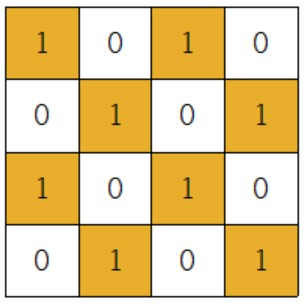
\includegraphics[width=4cm]{figure.jpg}
\end{figure}
\end{exer}

\begin{sol}
\begin{verbatim}

format short;
n=10;   % Set the size of the large check board

% Construct your checkboard
CheckBoard=zeros(n);    
CheckBoard(1:2:n, 1:2:n)=1;
CheckBoard(2:2:n, 2:2:n)=1;
for i=1:n
    Cn=CheckBoard(1:i, 1:i);
    [Qn Dn]=eig(Cn);    % Eigenvectors and eigenvalues
    fprintf('The size of the checkboard is %d \n',i);
    disp(diag(Dn)');
end
\end{verbatim}

\begin{outputs}

\begin{verbatim}

The size of the checkboard is 1 
     1
The size of the checkboard is 2 
     1 1
The size of the checkboard is 3 
     0 1 2
The size of the checkboard is 4 
     0 0 2 2
The size of the checkboard is 5 
   -0.0000 -0.0000  0.0000  2.0000  3.0000
The size of the checkboard is 6 
   -0.0000  -0.0000  -0.0000  -0.0000  3.0000  3.0000
The size of the checkboard is 7 
   -0.0000  -0.0000   0.0000   0.0000  0.0000  3.0000  4.0000
The size of the checkboard is 8 
   -0.0000  -0.0000  -0.0000  0.0000  0.0000  0.0000  4.0000  4.0000
The size of the checkboard is 9 
   -0.0000  -0.0000  -0.0000 -0.0000   0   0.0000  0.0000  4.0000  5.0000
The size of the checkboard is 10 
   -0.0000  -0.0000  -0.0000  0  0.0000  0.0000  0.0000  0.0000  5.0000  5.0000
\end{verbatim}
\end{outputs}


\noindent We may conclude that the eigenvalues of $C_{n}$ are given as follows:
$$\begin{cases} 1 &\text{if $n=1$,}\\ 
 k,\, k,\, \underbrace{0,\,0,\,\cdots,\,0}_{(n-2)}&\text{if $n=2k$,}\\
 k,\,k+1,\,\underbrace{0,\,0,\,\cdots,\,0}_{(n-2)}&\text{if $n=2k+1$,}
\end{cases}
$$ 
where $k$ is a positive integer.
\end{sol}

% section5
\chapter{Matrix Models}

%\vspace{5mm}
No MATLAB problems in this chapter.
%\vspace{20mm}
% section6
\chapter{Linear Transformations}

\section{Matrices as Transformations}

\begin{exer} (\textit{Linear Transformation: Rotation})\\
Make a function file with a function name \textit{reflect\_pt} to find the reflection of the point $(a,b)$ about the line through the origin of the $xy$-plane that makes an angle of $\theta\,^{\circ}$ with the positive $x$-axis. Make $a$, $b$, and $\theta$ the inputs to the function and the reflection point $(x,y)$ the output. Using this function, find the result of this function for $(a,b)=(1,3)$ and $\theta=12$ by the following commands:

\vspace{2mm}

\begin{verbatim}
>> [x, y]=reflect_pt(1, 3, 12)
\end{verbatim}

\end{exer}



\begin{sol}
\begin{verbatim}

%--- The following is the function file 'reflect_pt.m'. ---%
function [x, y]=reflect_pt(a, b, ang)
  theta=ang*(pi/180);
  T = [cos(2*theta) sin(2*theta); sin(2*theta) -cos(2*theta)];
    
  result=T*[a b]';
  x=result(1); y=result(2);
end
\end{verbatim}

\begin{outputs}

\begin{verbatim}

x =
    2.1338
    
y =
   -2.3339
\end{verbatim}
\end{outputs}
\end{sol}

\vspace{3mm}

\begin{exer} (\textit{Linear Transformation: Projection})\\ 
Consider successive rotations of $\mathbb{R}^{3}$ by an angle $\theta_{1}$ degree about the $x$-axis, then by an angle $\theta_{2}$ degree about the $y$-axis, and then by an angle $\theta_{3}$ degree about the $z$-axis. Make a function file named \textit{comp\_Rot} to find an appropriate axis and angle of rotation that achieves the same result in one rotation. Make $\theta_{1}, \theta_{2},$ and $\theta_{3}$ degrees the inputs to the function and the axis and angle of rotation the outputs. Give the output axis as a unit vector. You may make the standard matrix for the composition of the rotations by multiplication of the standard matrices for the rotations about the position $x$-, $y$-, and $z$-axes, respectively. Using the function \textit{comp\_Rot}, check the result of the following commands:

\vspace{2mm}

\begin{verbatim}
>> [L ang]=comp_Rot(45, 45, 45)
\end{verbatim}

\end{exer}


\begin{sol}

\begin{verbatim}

%--- The following is the function file 'comp_Rot.m'. ---%
function [L, ang] = comp_Rot(ang1, ang2, ang3)

  % Angle as a degree.
  angle=[ang1 ang2 ang3];

  % Convert angles from degrees to radians.
  theta=angle*(pi/180); 

  % Rotation about x-axis, y-axis, and z-axis.
  Rx = [1 0 0; 
        0 cos(theta(1)) -sin(theta(1)); 
        0 sin(theta(1)) cos(theta(1))];
  Ry = [cos(theta(2)) 0 sin(theta(2)); 
        0 1 0; 
        -sin(theta(2)) 0 cos(theta(2))];
  Rz = [cos(theta(3)) -sin(theta(3)) 0; 
        sin(theta(3)) cos(theta(3)) 0; 
        0 0 1];

  % Composition of the three rotation matrices R = Ry*Rx*Rz.
  R = Rz*Ry*Rx; 

  % Find the axis of rotation of R,
  % by finding the eigenvector of R 
  % corresponding to the eigenvalue lambda=1.

  % Find a nonzero vector satisfying Rx = x.
  L = null(eye(3) - R);

  % Make the axis of rotation unit vector. 
  L = L/norm(L);  

  % Find the angle of rotation of R.
  % Note that w=(-x2,x1,0) is 
  % orthogonal to the axis of rotation x=(x1,x2,x3).
  w = [-L(2) L(1) 0]';
  rot_theta = acos((dot(w, R*w))/((norm(w)*norm(R*w))));
  ang = ((rot_theta)*(180/pi));
end
\end{verbatim}


\begin{outputs}

\begin{verbatim}

L =
   -0.3574
   -0.8629
   -0.3574

ang =
   64.7368
\end{verbatim}
\end{outputs}

\end{sol}
\newpage

\section{Geometry of Linear Operators}

\begin{exer} (\textit{Rotation as an Orthogonal Transformation})\\
Let
\begin{displaymath}
A = \left[\begin{array}{rrrr} \displaystyle -\frac{3}{7}&\quad \displaystyle -\frac{2}{7}&\quad \displaystyle -\frac{6}{7} \vspace{3mm} \\ \vspace{3mm} \displaystyle \frac{6}{7} & \displaystyle -\frac{3}{7} & \displaystyle -\frac{2}{7}\\ \displaystyle -\frac{2}{7} & \displaystyle -\frac{6}{7} & \displaystyle \frac{3}{7} \end{array} \right].
\end{displaymath}

\vspace{2mm}
\noindent Show that $A$ represents a rotation, and use Formulas $(16)$ and $(17)$ in Section $6.2$ to find the axis and angle of rotation.
\end{exer}

\begin{sol}
\begin{verbatim}

A = [-3/7 -2/7 -6/7; 6/7 -3/7 -2/7; -2/7 -6/7 3/7]; format short;

% Check that A*A' is the identity matrix.
A*A' 

% Although the off diagonal entries are not exactly all zeros,
% the scaling factor suggests that roundoff error prevents
% the computed matrix from being the identity matrix.
% You can see that the product is exactly the identity matrix,
% when the symbolic computation is used.

% Check that det(A)=1 to conclude that A is orthogonal.
det(A) 

% Since A*A'=I and det(A) = 1, A represents a rotation.

% By (16) of Section 6.2,
% find the angle of rotation 
% and convert the angle from radians to degrees.
theta = acos((trace(A)-1)/2); ang = ((theta)*(180/pi));
disp('The angle of rotation in degrees is'); disp(ang);

% By (17) of Section 6.2, find the axis of rotation.
% The initial point at the origin.
e1 = [1 0 0]'; 

% v is along the axis of rotation.
v = (A+A'+((1-trace(A))*eye(3))) * e1; 
disp('The axis of rotation passes through the point'); disp(v');
\end{verbatim}


\begin{outputs}

\begin{verbatim}

The angle of rotation in degrees is
  135.5847
The axis of rotation passes through the point
    0.5714    0.5714   -1.1429
\end{verbatim}
\end{outputs}
\end{sol}



\section{Kernel and Range}


\begin{exer}
(\textit{Invertible Matrix as a Bijective Linear Transformation})\\
Consider the matrix
\begin{displaymath}
A = \left[\begin{array}{rrrr} 3& \hspace{1mm} -5& \hspace{1mm} -2&\hspace{3mm} 2\\ -4 & 7 & 4 & 4 \\ 4 & -9 & -3 & 7 \\ 2 & -6 & -3 & 2 \end{array} \right].
\end{displaymath}

\vspace{2mm}
Referring to the Theorem $6.3.15$ in Section $6.3$, show that $T_{A} : \mathbb{R}^{4} \rightarrow \mathbb{R}^{4}$ is onto in at least four different ways. You may use several related MATLAB commands.

\end{exer}


\begin{sol}
\begin{verbatim}

A = [3 -5 -2 2; -4 7 4 4; 4 -9 -3 7; 2 -6 -3 2];
format short;

% By (a) in Theorem 6.3.15, use the command rref of A.
rref(A)

% Since the reduced row echelon form of A is the identity matrix,
% the linear transformation T is onto.

% By (d) in Theorem 6.3.15, use the command null of A.

% Find a basis for the null space of A.
null(A, 'r') 

% Since the null space contains only the zero vector,
% the linear transformation T is onto.

% By (g) in Theorem 6.3.15, use the command rank of A.

% Find the number of linearly independent columns of A.
rank(A) 

% Since the column vectors of A are linearly independent,
% the linear transformation T is onto.

% By (i) in Theorem 6.3.15, use the command det of A.

% Find the determinant of A.
det(A) 

% Since det(A) is nonzero,
% the linear transformation T is onto.

% By (j) in Theorem 6.3.15, use the command eig of A.

% Find the eigenvalues A.
eig(A) 

% Since 0 is not an eigenvalue of A,
% the linear transformation T is onto.
\end{verbatim}
\end{sol}



\section{Composition and Invertibility of Linear Transformations}



\begin{exer}(\textit{Compositions of Linear Transformations})\\
Consider successive rotations of $\mathbb{R}^{3}$ by $30\,^{\circ}$ about the $z$-axis, then by $60\,^{\circ}$ about the $x$-axis, and then by $45\,^{\circ}$ about the $y$-axis. If it is desired to execute the three rotations by a single rotation about an appropriate axis, what axis and angle should be used?

\end{exer}


\begin{sol}
\begin{verbatim}

% Angle as a degree.
ang1=30; ang2=60; ang3=45; 

% Convert angles from degrees to radians.
theta1=((ang1)*(pi/180)); 
theta2=((ang2)*(pi/180));
theta3=((ang3)*(pi/180)); 

format short;

% Rotation about z-axis with the angle 30.
Rz = [cos(theta1) -sin(theta1) 0; sin(theta1) cos(theta1) 0; 0 0 1];
% Rotation about x-axis with the angle 60.
Rx = [1 0 0; 0 cos(theta2) -sin(theta2); 0 sin(theta2) cos(theta2)];
% Rotation about y-axis with the angle 45.
Ry = [cos(theta3) 0 sin(theta3); 0 1 0; -sin(theta3) 0 cos(theta3)];

% Composition of the three rotation matrices R = Ry*Rx*Rz.
R = Ry*Rx*Rz; 

% Find the axis of rotation of R,
% by finding the eigenvector of R corresponding to the eigenvalue lambda=1.

% Find a nonzero vector satisfying Rx = x.
x = null(eye(3) - R); 

% Find the angle of rotation of R.
% Note that w=(-x2,x1,0) is orthogonal to the axis of rotation x=(x1,x2,x3).
w = [-x(2) x(1) 0]';
theta = acos((dot(w, R*w))/((norm(w)*norm(R*w))));

% Convert the angle from radians to degrees.
ang = ((theta)*(180/pi));

disp('The angle of rotation in degrees is'); disp(ang);
disp('The axis of rotation is'); disp(x');
\end{verbatim}


\begin{outputs}

\begin{verbatim}

The angle of rotation in degrees is
   69.3559

The axis of rotation is
   -0.9350   -0.3525   -0.0391
\end{verbatim}

\end{outputs}
\end{sol}
% section7

\chapter{Dimension and Structure}

\section{Basis and Dimension}

\begin{exer} (\textit{Linear Combination and Independence})\\
Are any of the vectors in the set
\vspace{1mm}
\begin{displaymath}
S = \{ (2,6,3,4,2), \hspace{1.5mm}(3,1,5,8,3), \hspace{1.5mm}(5,1,2,6,7), \hspace{1.5mm}(8,4,3,2,6), \hspace{1.5mm}(5,5,6,3,4) \}
\end{displaymath}
\vspace{1mm}
linear combinations of predecessors? Justify your answer.

\end{exer}


\begin{sol}
\verb""
One strategy is to form a matrix $V$ of the column vectors $\mathbf{v}_{k}$ mentioned above and decide whether the system $V \mathbf{x} = \mathbf{0}$ has nontrivial solutions. If so, then at least one column is a linear combination of previous ones. Otherwise, the columns are linearly independent.

\begin{verbatim}

v1 = [2 6 3 4 2]'; v2 = [3 1 5 8 3]'; v3 = [5 1 2 6 7]';
v4 = [8 4 3 2 6]'; v5 = [5 5 6 3 4]';

% Construct V of the column vectors v1,v2,v3,v4 and v5.
V = [v1 v2 v3 v4 v5]; 

format short;

% Find the reduced row echelon form of V.
rref_V = rref(V); 

disp('The reduced row echelon form of A is'); disp(rref_V);
\end{verbatim}



\begin{outputs}

\begin{verbatim}

The reduced row echelon form of A is
     1     0     0     0     0
     0     1     0     0     0
     0     0     1     0     0
     0     0     0     1     0
     0     0     0     0     1
\end{verbatim}

\end{outputs}



\noindent Since the reduced row echelon form of $V$ has 5 pivots, the columns of V are linearly independent. Hence, no column of $V$ can be a linear combination of any other columns.
\end{sol}

\vspace{2mm}

\section{Properties of Bases}


\begin{exer}
In this problem, we make a function file \verb"CheckBasis.m" to check that the vectors $\mathbf{v}_{1}$, $\mathbf{v}_{2}$, $\mathbf{v}_{3}$ and $\mathbf{v}_{4}$ form a basis of $\mathbb{R}^4$ using the equivalent statements (a), (g), (h), and (o) of Theorem 7.2.7 in the textbook.

\begin{enumerate}
\item[(a)]
Complete the shadow part (/////) of the m-file given below referring to the comments and the execution results.

\begin{verbatim}

%--- your function file ---%
function [Result]=CheckBasis(v1, v2, v3, v4, case_num)
  %  if case_num=1, check the statement (a),
  %  if case_num=2, check the statement (g),
  %  if case_num=3, check the statement (h).

  % Construct the matrix V.
  ////////////////////////

  % Use the switch statement to check 
  % whether one of the statements (a), (g), and (h) holds.
  switch case_num
    case 1  
      fprintf('* You enter %d: statement (a) *\n', case_num);
      ////////////////////////
      if ////////////////////////
        disp('Given vectors form a basis of 4 dimensional space.');
      else
        disp('Given vectors do not form a basis of 4 dimensional space.');
      end
    case 2
      fprintf('* You enter %d: statement (g) *\n', case_num);
      Result=det(V);
      if Result~=0
        disp('Given vectors form a basis of 4 dimensional space.');
      else
        disp('Given vectors do not form a basis of 4 dimensional space.');
      end
    ///////////////////////////  % check statement (h)
        ////////////////////////
        ////////////////////////
        ////////////////////////
        ////////////////////////
        ////////////////////////
        ////////////////////////
        ////////////////////////
  end
end
\end{verbatim}

\vspace{3mm}

\noindent The execution results will be as follows:
\begin{verbatim}
>> v1=[1 0 0 0]'; v2=[0 2 0 0]'; v3=[0 0 4 5]'; v4=[0 0 0 -1]'; v5=[0 0 0 1]';
>> C=CheckBasis(v1, v2, v3, v4,3)
* You enter 3: statement (h) *
  Given vectors are basis of 4 dimensional space.

C =

     1
     2
    -1
     4

>> CheckBasis(v1, v2, v4, v5, 1);
* You enter 1: statement (a) *
  Given vectors do not form a basis of 4 dimensional space.

>> determinant=CheckBasis(v1, v2, v3, v5, 2)
* You enter 2: statement (g) *
  Given vectors form a basis of 4 dimensional space.

determinant =
     8
\end{verbatim}

\vspace{3mm}
\item[(b)] Using \verb"CheckBasis.m" from (a), check whether
\begin{itemize}
\item[i.] $\mathbf{v}_{1}=(-1, 0, 1, 0)^{T}$, $\mathbf{v}_{2}=(2, 3, -2, 6)^{T}$, $\mathbf{v}_{3}=(0, -1, 2, 0)^{T}$ and $\mathbf{v}_{4}=(0, 0, 1, 5)^{T}$ form a basis of $\mathbb{R}^4$.

\item[ii.] $\mathbf{v}_{1}=(a, b, c, d)^{T}$, $\mathbf{v}_{2}=(-b, a, d, -c)^{T}$, $\mathbf{v}_{3}=(-c, -d, a, b)^{T}$ and $\mathbf{v}_{4}=(-d, c, -b, a)^{T}$ form a basis of $\mathbb{R}^4$. (Do not use the statement (h). Guess why not?)
\end{itemize}

\end{enumerate}
\end{exer}


\begin{sol}

\vspace{1mm}
\verb""
\begin{enumerate}
\item[(a)]
\verb" "
\verb"% ----- your function file ----- %"\\
\verb"function [Result]=CheckBasis(v1, v2, v3, v4, case_num)"\\
\verb"  %  if case_num=1, check the statement (a),"\\
\verb"  %  if case_num=2, check the statement (g),"\\
\verb"  %  if case_num=3, check the statement (h)."\\
\\
\verb" % Construct the matrix V."\\
  \textcolor{blue}{\texttt{  V=[v1 v2 v3 v4];}}\\

\verb"  % Use the switch statement to check" \\
\verb"  % whether one of the statements (a), (g), and (h) holds."\\
\verb"  switch case_num"\\
\verb"    case 1"  \\
\verb"      fprintf('* You enter %d: statement (a) *', case_num);"\\
\textcolor{blue}{\texttt{ \hspace{8mm}         Result=rref(V)}}

\hspace{8mm}      \texttt{ if \textcolor{blue}{det(Result)$\sim$=0}}\\
\verb"        disp('Given vectors form a basis of 4 dimensional space.');"\\
\verb"      else"\\
\verb"        disp('Given vectors do not form a basis of 4 dimensional space.');"\\
\verb"      end"\\
\verb"    case 2"\\
\verb"      fprintf('* You enter %d: statement (g) *', case_num);"\\
\verb"      Result=det(V);"\\
\verb"      if Result~=0"\\\
\verb"        disp('Given vectors form a basis of 4 dimensional space.');"\\
\verb"      else"\\
\verb"        disp('Given vectors do not form a basis of 4 dimensional space.');"\\
\verb"      end"\\
\textcolor{blue}{\texttt{  \hspace{4mm}  case 3}}\verb"  % check statement (h)"\\
\textcolor{blue}{\texttt{  \hspace{8mm}      [Q D]=eig(V);}}

\textcolor{blue}{\texttt{  \hspace{8mm}            Result=diag(R);}}

\textcolor{blue}{\texttt{  \hspace{8mm}         if det(R)==0}}

\textcolor{blue}{\texttt{   \hspace{12mm}       disp('Given vectors form a basis of 4 dimensional space.');}}

\textcolor{blue}{\texttt{  \hspace{8mm}              else}}

 \textcolor{blue}{\texttt{  \hspace{12mm}               disp('Given vectors do not form a basis of 4 dimensional space.');}}

\textcolor{blue}{\texttt{  \hspace{8mm}        end}}

\textcolor{blue}{\texttt{  \hspace{4mm}      end}}


\item[(b)-i.] 
\begin{verbatim}
>> v1=[-1 0 1 0]'; v2=[2 3 -2 6]';  v3=[0 -1 2 0]'; v4 = [0 0 1 5]';
>> CheckBasis(v1, v2, v3, v4, 1);
>> CheckBasis(v1, v2, v3, v4, 2);
>> CheckBasis(v1, v2, v3, v4, 3);
\end{verbatim}

\begin{outputs}
\begin{verbatim}

* You enter 1: statement (a) *
  Given vectors form a basis of 4 dimensional space.
* You enter 2: statement (g) *
  Given vectors form a basis of 4 dimensional space.
* You enter 3: statement (h) *
  Given vectors form a basis of 4 dimensional space.
\end{verbatim}
\end{outputs}

\item[(b)-ii.] 
\begin{verbatim}
>> syms a b c d;
>> v1=[a;b;c;d]; v2=[-b;a;d;-c]; v3=[-c;-d;a;b]; v4 = [-d;c;-b;a];
>> CheckBasis(v1, v2, v3, v4, 1);
>> CheckBasis(v1, v2, v3, v4, 2);
\end{verbatim}

\begin{outputs}
\begin{verbatim}

* You enter 1: statement (a) *
  Given vectors form a basis of 4 dimensional space.
* You enter 2: statement (g) *
  Given vectors form a basis of 4 dimensional space.
\end{verbatim}
\end{outputs}
\end{enumerate}
\end{sol}



\section{The Fundamental Spaces of a Matrix}


\begin{exer}\label{ex1}
In this problem, we make a function file \verb"getFSinfo.m" to get the dimension and basis of the fundamental spaces of a given matrix. For example, we execute the followings:
\begin{verbatim}
>> A=[1 0 0 0 2; -2 1 -3 -2 -4; 0 5 -14 -9 0; 2 10 -28 -18 4];
>> getFSinfo(A);
\end{verbatim}
Then, the Command Window displays the results as follows:
\begin{verbatim}
Given matrix is:
     1     0     0     0     2
    -2     1    -3    -2    -4
     0     5   -14    -9     0
     2    10   -28   -18     4

== Dimension of the fundamental spaces of a given matrix ==
dim(row(A))=dim(col(A)): 3, 	 dim(null(A)): 2, 	 dim(null(A_trans)): 1

== Basis of the fundamental spaces of a given matrix (in row vectors) ==
 row(A)
     1     0     0     0     2
     0     1     0     1     0
     0     0     1     1     0

 col(A)
     1     0     0     2
     0     1     0     0
     0     0     1     2

 null(A)
     0    -1    -1     1     0
    -2     0     0     0     1

 null(A_trans)
    -2     0    -2     1

*****************************************************
\end{verbatim}
\begin{enumerate}
\item[(a)] Complete the missing parts of the m-file \verb"getFSinfo" given as follows:
\begingroup
    \fontsize{10pt}{12pt}\selectfont
\begin{verbatim}

%--- function file 'getFSinfo.m' ---%
function [info]=getFSinfo(A)
  % row(A): basis and dimension
  /////// missing part ///////

  % col(A): basis and dimension
  /////// missing part ///////

  % null(A): basis and dimension
  /////// missing part ///////

  % null(A'): basis and dimension
  /////// missing part ///////

  disp('Given matrix is:'); disp(A);
  fprintf('== Dimension of the fundamental spaces of given matrix == \n');
  fprintf('dim(row(A))=dim(col(A)): %d,', rank_A);
  fprintf('\t dim(null(A)): %d,\t dim(null(A_trans)): %d \n\n', nullity, nullity_T);
  fprintf('== Basis of the fundamental spaces of given matrix (in row vectors) == \n');
  disp(' row(A)'); disp(double(rowA_basis));
  disp(' col(A)'); disp(double(colA_basis));
  disp(' null(A)'); disp(nullA_basis);
  disp(' null(A_trans)'); disp(nullAtrans_basis);
  fprintf('\n*****************************************************\n');
end
\end{verbatim}
\endgroup
You may use the MATLAB commands \textit{rank, colspace, rref, null} and so on.
\vspace{3mm}
\item[(b)] Using your function file \verb"getFSinfo.m", find the dimension and basis of the fundamental spaces of

$A = \begin{bmatrix} 3 & 2& 1& 3& 5 \\ 6& 4& 3& 5& 7 \\ 9&6&5&7&9\\3&2&0&4&8 \end{bmatrix}$, $B = \begin{bmatrix} 3 & -1 & 3& 2& 5 \\ 5& -3&2&3&4\\ 1&-3&-5&0& -7\\ 7&-5&1&4&1\end{bmatrix}$, $C = \begin{bmatrix} 1& 3& 2& 1\\ -2 & -6 & 0& -6\\ 3& 9& 1& 8\\ -1& -3& -3& -6\\ 1& 3& 2& 1\\ 4& 12& 1&11 \end{bmatrix}$.
\end{enumerate}
\end{exer}

\begin{sol}
\verb""
\begin{enumerate}
\item[(a)]

\verb"% ----- function file 'getFSinfo.m' ----- %"

\verb"function [info]=getFSinfo(A)"

\verb"  [m,n]=size(A)"

\verb"  % row(A): basis and dimension"

{\color{blue}\verb"    rank_A=rank(A);    % rank of A;"

    \verb"    rowA=colspace(sym(A')); % find the row basis"

    \verb"    rowA_basis=rowA(:, 1:rank_A)';  % basis of row(A)"
    }



\verb"  % col(A): basis and dimension"

{\color{blue}\verb"    colA=colspace(sym(A)); % find the column basis"

\verb"    colA_basis=colA(:, 1:rank_A)';  % basis of col(A)"
    }




\verb"  % null(A): basis and dimension"

{\color{blue}\verb"    nullA=null(A, 'r');"

\verb"    nullity=n-rank_A;   % using Dimension theorem"

\verb"    nullA_basis=nullA(:, 1:nullity)';"
    }

\verb"  % null(A'): basis and dimension"

{\color{blue}\verb"    nullAtrans=null(A', 'r');"

    \verb"    nullity_T=m-rank_A;    "

    \verb"    nullAtrans_basis=nullAtrans(:,1:nullity_T)';"
    }
\begin{verbatim}
  disp('Given matrix is:'); disp(A);
  fprintf('== Dimension of the fundamental spaces of given matrix == \n');
  fprintf('dim(row(A))=dim(col(A)): %d,', rank_A);
  fprintf('\t dim(null(A)): %d,', nullity);
  fprintf('\t dim(null(A_trans)): %d \n\n', nullity_T);
  fprintf('== Basis of the fundamental spaces ');
  fprintf('of given matrix (in row vectors) == \n');
  disp(' row(A)'); disp(double(rowA_basis));
  disp(' col(A)'); disp(double(colA_basis));
  disp(' null(A)'); disp(nullA_basis);
  disp(' null(A_trans)'); disp(nullAtrans_basis);
  fprintf('\n*****************************************************\n');
end
\end{verbatim}

\item[(b)]
\begin{verbatim}
A=[3 2 1 3 5; 6 4 3 5 7; 9 6 5 7 9; 3 2 0 4 8];
B=[3 -1 3 2 5; 5 -3 2 3 4; 1 -3 -5 0 -7; 7 -5 1 4 1];
C=[1 3 2 1; -2 -6 0 -6 ;3 9 1 8; -1 -3 -3 -6; 1 3 2 1; 4 12 1 11];
getFSinfo(A);
getFSinfo(B);
getFSinfo(C);
\end{verbatim}


\begin{outputs}
\begin{verbatim}

Given matrix is:
     3     2     1     3     5
     6     4     3     5     7
     9     6     5     7     9
     3     2     0     4     8
== Dimension of the fundamental spaces of given matrix ==
dim(row(A))=dim(col(A)): 2,	 dim(null(A)): 3,	 dim(null(A_trans)): 2
== Basis of the fundamental spaces of given matrix (in row vectors) ==
 row(A)
    1.0000    0.6667         0    1.3333    2.6667
         0         0    1.0000   -1.0000   -3.0000
 col(A)
     1     0    -1     3
     0     1     2    -1
 null(A)
   -0.6667    1.0000         0         0         0
   -1.3333         0    1.0000    1.0000         0
   -2.6667         0    3.0000         0    1.0000
 null(A_trans)
     1    -2     1     0
    -3     1     0     1
*****************************************************

Given matrix is:
     3    -1     3     2     5
     5    -3     2     3     4
     1    -3    -5     0    -7
     7    -5     1     4     1
== Dimension of the fundamental spaces of given matrix ==
dim(row(A))=dim(col(A)): 3,	 dim(null(A)): 2,	 dim(null(A_trans)): 1
== Basis of the fundamental spaces of given matrix (in row vectors) ==
 row(A)
    1.0000         0    1.7500    0.7500         0
         0    1.0000    2.2500    0.2500         0
         0         0         0         0    1.0000
 col(A)
     1     0    -3     0
     0     1     2     0
     0     0     0     1
 null(A)
   -1.7500   -2.2500    1.0000         0         0
   -0.7500   -0.2500         0    1.0000         0
 null(A_trans)
     3    -2     1     0
*****************************************************

Given matrix is:
     1     3     2     1
    -2    -6     0    -6
     3     9     1     8
    -1    -3    -3    -6
     1     3     2     1
     4    12     1    11
== Dimension of the fundamental spaces of given matrix ==
dim(row(A))=dim(col(A)): 3,	 dim(null(A)): 1,	 dim(null(A_trans)): 3
== Basis of the fundamental spaces of given matrix (in row vectors) ==
 row(A)
     1     3     0     0
     0     0     1     0
     0     0     0     1
 col(A)
    1.0000         0    0.5000         0    1.0000    0.5000
         0    1.0000   -1.2500         0         0   -1.7500
         0         0         0    1.0000         0         0
 null(A)
    -3     1     0     0
 null(A_trans)
   -0.5000    1.2500    1.0000         0         0         0
   -1.0000         0         0         0    1.0000         0
   -0.5000    1.7500         0         0         0    1.0000
*****************************************************
\end{verbatim}
\end{outputs}
\end{enumerate}
\end{sol}

\vspace{3mm}

\begin{exer}
(\textit{Bases for the Fundamental Spaces})

\begin{enumerate}

\item[(a)] Use the MATLAB commands \textit{sym} and \textit{colspace} to find a basis for the column space of the matrix

\begin{displaymath}
A = \left[\begin{array}{rrrr} 2& \hspace{2mm} -1& \hspace{5mm} 3&\hspace{4mm} 5\\ 4 & -3 & 1 & 3 \\ 3 & -2 & 3 & 4 \\ 4 & -1 & 15 & 17 \\ 7 & -6 & -7 & 0 \end{array} \right].
\end{displaymath}

\vspace{1mm}

\item[(b)] Use the same MATLAB commands in (a) to find a basis for the row space of $A$.

\vspace{1mm}

\item[(c)] Confirm that the basis obtained in (b) is consistent with the basis obtained from the reduced row echelon form of $A$.

\vspace{1mm}

\item[(d)] Tell what happens if you use the MATLAB command \textit{orth}?

\end{enumerate}
\end{exer}



\begin{sol}
\verb""

%\vspace{3mm}


\begin{itemize}
\item[(a)]
\begin{verbatim}
% Set a matrix A whose entries are symbolic objects.
A = sym([2 -1 3 5; 4 -3 1 3; 3 -2 3 4; 4 -1 15 17; 7 -6 -7 0]);

% Find a basis for the column space of A.
col_basis = colspace(A);

disp('A basis for the column space of A is');
disp(col_basis(:,1)'); disp(col_basis(:,2)'); disp(col_basis(:,3)');
\end{verbatim}


\begin{outputs}
\begin{verbatim}

A basis for the column space of A is
[ 1, 0, 0, 2, 1]

[ 0, 1, 0, -3, 5]

[ 0, 0, 1, 4, -5]
\end{verbatim}
\end{outputs}


\item[(b)]
\begin{verbatim}
% Set a matrix A_transpose whose entries are symbolic objects.
A_transpose = sym([2 -1 3 5; 4 -3 1 3; 3 -2 3 4; 4 -1 15 17; 7 -6 -7 0]');

% Finding a basis for the row space of A is equivalent to
% finding a basis for the column space of A_transpose.
rowbasis = colspace(A_transpose);

disp('A basis for the row space of A is');
disp(rowbasis(:,1)'); disp(rowbasis(:,2)'); disp(rowbasis(:,3)');
\end{verbatim}



\begin{outputs}
\begin{verbatim}

A basis for the row space of A is
[ 1, 0, 0, 6]

[ 0, 1, 0, 7]

[ 0, 0, 1, 0]
\end{verbatim}
\end{outputs}



\item[(c)]
\begin{verbatim}
% Set a matrix A.
A = [2 -1 3 5; 4 -3 1 3; 3 -2 3 4; 4 -1 15 17; 7 -6 -7 0];

% Find the reduced row echelon form of A.
rref_A = rref(A); 

% The nonzero rows of the reduced row echelon form of A
% form a basis for the row space of A.

disp('A basis for the row space of A is');
disp(rref_A(1,:)); disp(rref_A(2,:)); disp(rref_A(3,:));
\end{verbatim}

\begin{outputs}
\begin{verbatim}

A basis for the row space of A is
     1     0     0     6

     0     1     0     7

     0     0     1     0
\end{verbatim}
\end{outputs}

\item[(d)]

\begin{verbatim}
% Set A.
A = [2 -1 3 5; 4 -3 1 3; 3 -2 3 4; 4 -1 15 17; 7 -6 -7 0]; 

% The command orth gives an orthonormal basis for the column space of A.
B = orth(A);

disp('An orthonormal basis for the column space of A is');
disp('q1='); disp(B(:,1)');
disp('q2='); disp(B(:,2)');
disp('q3='); disp(B(:,3)');
\end{verbatim}

\begin{outputs}
\begin{verbatim}

An orthonormal basis for the column space of A is
q1=
   -0.2427   -0.1508   -0.2229   -0.9246    0.1177

q2=
   -0.1189   -0.3624   -0.2060    0.0253   -0.9008

q3=
    0.3760   -0.6016   -0.5930    0.1848    0.3331
\end{verbatim}
\end{outputs}
\end{itemize}
\end{sol}

\section{The Dimension Theorem and Its Implications}


\begin{exer}
(\textit{Rank and Nullity})

\begin{enumerate}

\item[(a)] Use the MATLAB command \textit{rank} and the Formula (2) in Section $7.4$ to find the nullity of the matrix

\begin{displaymath}
A = \left[\begin{array}{rrrrr} 3& \hspace{1mm} 2& \hspace{1mm} 1&\hspace{1mm} 3&\hspace{1mm} 5\\ 6 & 4 & 3 & 5 & 7 \\ 9 & 6 & 5 & 7 & 9 \\ 3 & 2 & 0 & 4 & 8 \end{array} \right].
\end{displaymath}


\item[(b)] Confirm that the result obtained in (a) is consistent with the number of basis vectors which are obtained by using the MATLAB command \textit{null}.

\end{enumerate}

\end{exer}


\begin{sol}
\verb""
\begin{itemize}


\item[(a)]

\begin{verbatim}
% Set A.
A = [3 2 1 3 5; 6 4 3 5 7; 9 6 5 7 9; 3 2 0 4 8]; 

% Find the rank of A by using the command rank.
rank_A = rank(A); 

% Size of the matrix A.
[ m n ] = size(A); 
% m = the number of rows of A, n = the number of columns of A.

 % By (2) in section 7.4, rankA + nullA = n.
null_A = n - rank_A;

disp('The nullity of A is'); disp(null_A);
\end{verbatim}

\begin{outputs}
\begin{verbatim}

The nullity of A is
     3
\end{verbatim}
\end{outputs}


\item[(b)]
\begin{verbatim}
% Set A.
A = [3 2 1 3 5; 6 4 3 5 7; 9 6 5 7 9; 3 2 0 4 8]; 

% Find a basis for the null space of A.
nullA = null(A,'r'); 
% null(A,'r') returns a matrix 
% whose columns are a basis for the null space of A.

[m n] = size(nullA);
% Since the number of columns of nullA is n,
% thus, n = the number of basis vectors of the null space of A.

disp('The nullity of A is'); disp(n);
\end{verbatim}


\begin{outputs}
\begin{verbatim}

The nullity of A is
     3
\end{verbatim}
\end{outputs}





\end{itemize}

\end{sol}




\section{The Rank Theorem and Its Implications}

\begin{exer}
Note that the rank of a nonzero matrix $A$ is equal to the order of the largest square submatrix of $A$ (formed by deleting rows and columns of $A$) whose determinant is nonzero. In this problem, we make a function file \verb"CheckRank.m" to find the rank of the given matrix using this fact. We want to obtain the execution results as follows:
\begin{verbatim}
>> A=[1 2 3 4; 5 6 7 8; 9 10 11 12; 13 14 15 16];
>> rankA=CheckRank(A)
rankA =
     2
\end{verbatim}
For this, you may start with the largest square matrices to be found in $A$ and a search is started for the first submatrix with a nonzero determinant. Use the MATLAB command \textit{nchoosek} to select all the combinations of rows and columns needed in the search process and you may use the several MATLAB commands if you need. Complete the m-file below and check the determinant of the matrices $A$, $B$, and $C$ given in the Exercise \ref{ex1} (b). Also, compare the results using the MATLAB command \textit{rank}.
\end{exer}


\begin{sol}
\begin{verbatim}

%--- function file 'CheckRank.m' ---%
function [rank_A]= CheckRank(A)
\end{verbatim}

{\color{blue}
\begin{verbatim}
    [m,n]=size(A);  % size of given matrix
    flg=1;  % flag for while loop
    if m>n  % if (# of row) > (# of col)
        A=A';
    end
    A=sym(A);   % Set A as a symbolic object

    K = min(m,n);   N = max(m,n);   % k : row number, N: col number
    k=K;    % from the largest size of submatrix
    while flg == 1
        comb_row=nchoosek(1:K, k);  % combinations of row
        comb_col=nchoosek(1:N, k);  % combinations of columns
        for ii=1:size(comb_row) %
            selected_A=A(comb_row(ii,:),:); % selected row index
            for jj=1:size(comb_col)
                sub_A=selected_A(:,comb_col(jj, :));   % selected col index
                if det(sub_A)~=0    % if non zeros determinant appears
                    rank_A=k;   % the size at that time <- rank
                    flg=0;  % stop the while loop.
                end
            end
        end
        k=k-1;  % if all submatrices of size k have a zero determinant,
                % reduce the size of submatrix.
    end
\end{verbatim}}
\begin{verbatim}
end
\end{verbatim}


\noindent To check the determinant of the matrices $A$, $B$, and $C$ given in the Exercise \ref{ex1}, you execute the followings:
\begin{verbatim}
A=[3 2 1 3 5; 6 4 3 5 7; 9 6 5 7 9; 3 2 0 4 8];
B=[3 -1 3 2 5; 5 -3 2 3 4; 1 -3 -5 0 -7; 7 -5 1 4 1];
C=[1 3 2 1; -2 -6 0 -6 ;3 9 1 8; -1 -3 -3 -6; 1 3 2 1; 4 12 1 11];

fprintf('my rank(A): %.5f, MATLAB rank(A): %.5f \n', CheckRank(A), rank(A));
fprintf('my rank(B): %.5f, MATLAB rank(B): %.5f \n', CheckRank(B), rank(B));
fprintf('my rank(C): %.5f, MATLAB rank(C): %.5f \n', CheckRank(C), rank(C));
\end{verbatim}

\begin{outputs}
\begin{verbatim}

my rank(A): 2.00000, MATLAB rank(A): 2.00000
my rank(B): 3.00000, MATLAB rank(B): 3.00000
my rank(C): 3.00000, MATLAB rank(C): 3.00000
\end{verbatim}
\end{outputs}

\noindent Those are the same results as given in Exercise\ref{ex1}.

\end{sol}


% 7.6
\section{The Pivot Theorem and Its Implications}


\begin{exer}(\textit{Finding a Basis with the Pivot Theorem})\\
Consider the vectors
\begin{displaymath}
\begin{array}{lll} \vspace{1mm} \hspace{2mm} \mathbf{v}_{1} & \hspace{1mm} = & \hspace{1mm} (1, \hspace{1mm} 2, \hspace{1mm} 4, \hspace{1mm} -6,  \hspace{1mm} 11, \hspace{1mm} 23, \hspace{1mm} -14, \hspace{1mm} 0, \hspace{1mm} 2, \hspace{1mm} 2), \\ \vspace{1mm} \hspace{2mm} \mathbf{v}_{2} & \hspace{1mm} = & \hspace{1mm} (3, \hspace{1mm} 1, \hspace{1mm} -1, \hspace{1mm} 7, \hspace{1mm} 9, \hspace{1mm} 13, \hspace{1mm} -12, \hspace{1mm} 8, \hspace{1mm} 6, \hspace{1mm} -30), \\ \vspace{1mm} \hspace{2mm} \mathbf{v}_{3} & \hspace{1mm} = & \hspace{1mm} (5, \hspace{1mm} 5, \hspace{1mm} 7, \hspace{1mm} -5, \hspace{1mm} 31, \hspace{1mm} 59, \hspace{1mm} -40, \hspace{1mm} 8, \hspace{1mm} 10, \hspace{1mm}-26), \\ \vspace{1mm} \hspace{2mm} \mathbf{v}_{4} & \hspace{1mm} = & \hspace{1mm} (5, \hspace{1mm} 0, \hspace{1mm} -6, \hspace{1mm} 20, \hspace{1mm} 7, \hspace{1mm} 3, \hspace{1mm} -10, \hspace{1mm} 16, \hspace{1mm} 10, \hspace{1mm} -62). \end{array}
\end{displaymath}
Use Algorithm $1$ in Section $7.6$ to find a subset of these vectors that forms a basis for span$\{\mathbf{v}_{1}, \mathbf{v}_{2}, \mathbf{v}_{3}, \mathbf{v}_{4}\}$, and express those vectors not in the basis as linear combinations of basis vectors.
\end{exer}

\begin{sol}


\begin{verbatim}

v1 = [1 2 4 -6 11 23 -14 0 2 2]';
v2 = [3 1 -1 7 9 13 -12 8 6 -30]';
v3 = [5 5 7 -5 31 59 -40 8 10 -26]';
v4 = [5 0 -6 20 7 3 -10 16 10 -62]';

% Construct A whose column space is W=span(v1,v2,v3,v4).
A = [v1 v2 v3 v4];

% Find the reduced row echelon form R of A and the pivot columns of A.
[R, pivotcols] = rref(A);

format short;

disp('The pivot columns of the reduced row echelon form of A are');
disp(pivotcols);

% From the result, the leading 1's in R occur in columns 1 and 2.
% (i.e., the pivot columns of A are 1 and 2.)
% Hence, the basis vectors for W are v1 and v2.

disp('The reduced row echelon form R of A is'); disp(R);

% Furthermore, from the reduced row echelon form R of A,
% we can see that v3 = 2*v1 + v2, and v4 = -v1 + 2*v2.
\end{verbatim}

\begin{outputs}
\begin{verbatim}

The pivot columns of the reduced row echelon form of A are
     1     2

The reduced row echelon form R of A is
     1     0     2    -1
     0     1     1     2
     0     0     0     0
     0     0     0     0
     0     0     0     0
     0     0     0     0
     0     0     0     0
     0     0     0     0
     0     0     0     0
     0     0     0     0
\end{verbatim}
\end{outputs}

\end{sol}

\vspace{3mm}


\begin{exer}(\textit{Finding Bases for the Fundamental Spaces})\\
Consider the matrix

\begin{displaymath}
A = \left[\begin{array}{rrrr} 1& \hspace{5mm} 3& \hspace{5mm} 2&\hspace{5mm} 1\\ -2 & -6 & 0 & -6 \\ 3 & 9 & 1 & 8 \\ -1 & -3 & -3 & -6 \\ 1 & 3 & 2 & 1 \\ 4 & 12 & 1 & 11 \end{array} \right].
\end{displaymath}

\begin{enumerate}

\item[(a)] Use Algorithm 1 in Section 7.6 to find a subset of the column vectors of $A$ that forms a basis for the column space of $A$, and express each column vector of $A$ that is not in that basis as a linear combination of the basis vectors.

\vspace{2mm}

\item[(b)] Use Algorithm 2 in Section 7.6 to find a basis for the null space of the matrix $A^{T}$.
\end{enumerate}

\end{exer}


\begin{sol}
\begin{verbatim}

A = [1 3 2 1; -2 -6 0 -6; 3 9 1 8; -1 -3 -3 -6; 1 3 2 1; 4 12 1 11];

% Find the reduced row echelon form R of A and the pivot columns of A.
[R, pivotcols] = rref(A);

format short;

disp('The pivot columns of the reduced row echelon form of A are');
disp(pivotcols);
% From the result, the leading 1's in R occur in columns 1, 3, and 4.
% (i.e., the pivot columns of A are 1, 3, and 4.)
% Hence, the columns 1, 3, and 4 of A are a basis for the column space of A.

disp('The reduced row echelon form R of A is'); disp(R);
% Furthermore, from the reduced row echelon form R of A,
% we can see that v2 = 3*v1, where v1 = A(:, 1), and v2 = A(:, 2).
\end{verbatim}


\begin{outputs}
\begin{verbatim}

The pivot columns of the reduced row echelon form of A are
     1     3     4

The reduced row echelon form R of A is
     1     3     0     0
     0     0     1     0
     0     0     0     1
     0     0     0     0
     0     0     0     0
     0     0     0     0
\end{verbatim}
\end{outputs}

\end{sol}








% 7.7
\section{The Projection Theorem and Its Implications}


\begin{exer}(\textit{Standard Matrix for an Orthogonal Projection})\\
One way to find the standard matrix for the orthogonal projection onto a subspace $W$ spanned by a set of vectors $\{\mathbf{v}_{1}, \mathbf{v}_{2}, ..., \mathbf{v}_{k}\}$ is first to find a basis for $W$, then create a matrix $A$ that has the basis vectors as columns, and then use the Formula (27) in the Section 7.7.

\vspace{2mm}

\begin{enumerate}

\item[(a)] Find the standard matrix for the orthogonal projection of $\mathbb{R}^{4}$ onto the subspace $W$ spanned by

\begin{displaymath}
\begin{array}{ll} \vspace{1mm} \mathbf{v}_{1} = (1, \hspace{1mm} 2, \hspace{1mm} 3, \hspace{1mm} -4), & \hspace{2mm} \mathbf{v}_{2} = (2, \hspace{1mm}3, \hspace{1mm} -4, \hspace{1mm} 1), \\ \vspace{1mm} \mathbf{v}_{3} = (2, \hspace{1mm} -5, \hspace{1mm} 8, \hspace{1mm} -3), & \hspace{2mm} \mathbf{v}_{4} = (5, \hspace{1mm} 26, \hspace{1mm} -9, \hspace{1mm} -12), \\ \vspace{1mm} \mathbf{v}_{5} = (3, \hspace{1mm} -4, \hspace{1mm} 1, \hspace{1mm} 2). \end{array}
\end{displaymath}

\vspace{1mm}

\item[(b)] Use the matrix obtained in part (a) to find $\mathrm{proj}_{\tiny{W}} \mathbf{x}$, where $\mathbf{x} = (1, \hspace{1mm} 0, \hspace{1mm} -3, \hspace{1mm} 7)$.

\vspace{3mm}

\item[(c)] Find $\mathrm{proj}_{\tiny{W^{\perp}}} \mathbf{x}$ for the vector in part (b).

\end{enumerate}
\end{exer}

\begin{sol}
\begin{verbatim}

v1 = [1 2 3 -4]'; v2 = [2 3 -4 1]'; v3 = [2 -5 8 -3]';
v4 = [5 26 -9 -12]'; v5 = [3 -4 1 2]';

% Set A that has v1,v2,v3,v4 and v5, as column vectors.
A = [v1 v2 v3 v4 v5]; 

% Find the reduced row echelon form R of A and the pivot columns of A.
[R, pivotcols] = rref(A);

% M is the matrix whose columns are a basis for the column space of A.
M = A(:, pivotcols);

% By (27) in section 7.7, find the standard matrix.
P = M * inv(M'* M) * M';

format short;
disp('The standard matrix for the orthogonal projection of R^4 onto W=col(A) is');
disp(P);

x = [1 0 -3 7]'; 
xproj = P*x; 
xperp = x - xproj;
disp('The projection of x onto W=col(A) is'); disp(xproj');

disp('The projection of x onto the orthogonal complement of W=col(A) is');
disp(xperp');

% As a check, the dot product of the two projections should be zero.
disp('The dot product of the two projections is'); disp(dot(xproj, xperp));
\end{verbatim}


\begin{outputs}
\begin{verbatim}

The standard matrix for the orthogonal projection of R^4 onto W=col(A) is
    0.9992   -0.0144   -0.0161   -0.0195
   -0.0144    0.7551   -0.2737   -0.3314
   -0.0161   -0.2737    0.6941   -0.3703
   -0.0195   -0.3314   -0.3703    0.5517

The projection of x onto W=col(A) is
    0.9110   -1.5127   -4.6907    4.9534

The projection of x onto the orthogonal complement of W=col(A) is
    0.0890    1.5127    1.6907    2.0466

The dot product of the two projections is
 -5.3291e-015
\end{verbatim}
\end{outputs}

\end{sol}

% 7.8
\section{Best Approximation and Least Squares}

\begin{exer}
Make a function file \verb"LinearSolver.m" to find a least squares solution of $A\mathbf{x}=\mathbf{b}$ where $A$ has full column rank. Complete the missing part referring to the comments. Using this function file, solve the linear system
$$\begin{cases}
x-y=4\\
3x+2y=1\\
-2x+4y=3
\end{cases}
$$
and compare the output with the result of the MATLAB syntax $A\backslash \mathbf{b}$.
\end{exer}


\begin{sol}

\begin{verbatim}

%--- This is a function file 'LinearSolver.m' ---%
function [rank_A sol]=LinearSolver(A, b)
  [m,n]=size(A);
  rank_A=rank(A);
    
  % Check that A has full column rank.   
  if rank_A<n
    fprintf('rank(A)=%d < %d  -> Not full column rank\n', rank_A, n);
    return; % If A does not have full column rank, then return.
  else 
    fprintf('rank(A)=%d = %d -> Full column rank\n', rank_A, n);
  end
   
  % From the reduced row echelon form of [A'*A |A'*b],
  % find a solution to the normal equation A'Ax=A'b.

  Aug=[A'*A A'*b]; 
  rref_Aug=rref(Aug);
  sol=rref_Aug(:,n+1);
  
  fprintf('The least squares solution is');disp(sol');
end
\end{verbatim}

You execute the followings:
\begin{verbatim}
A=[1 -1; 3 2; -2 4];   
b=[4; 1; 3];
LinearSolver(A, b);
A\b
\end{verbatim}

\begin{outputs}
\begin{verbatim}

rank(A)=2 = 2 -> Full column rank
The least squares solution is    0.1789    0.5018
ans =
    0.1789
    0.5018
\end{verbatim}

\end{outputs}

\end{sol}

\vspace{3mm}

\begin{exer}
The least squares method can be used to estimate the center $(h,k)$ of a circle $(x-h)^2+(y-k)^2=r^2$ using measured data points on its circumference. Suppose that the data points are
$$(x_1, y_1), (x_2, y_2), \cdots, (x_n, y_n)$$
and rewrite the equation of the circle in the form
\begin{equation}\label{eq1}\centering  2xh+2yk+s=x^2+y^2
\end{equation}
where
\begin{equation}\label{eq2}\centering s=r^2-h^2-k^2\end{equation}
Substituting the data points in \eqref{eq1} yields a linear system in the unknowns $h$, $k$, and $s$, which can be solved by least squares to estimate their values. Equation~\eqref{eq2} can then be used to estimate $r$. Use this method to approximate the center and radius of a circle from the measured data points on the circumference given in the accompanying table.

\begin{table}[h]
\centering
\caption{Data points of Problem 7(b)}
\label{my-label}
\begin{tabular}{|l|l|l|l|l|l|l|l|}
\hline
$\mathbf{x}$ & 19.880 & 20.919 & 21.735 & 23.375 & 24.361 & 25.375 & 25.979 \\ \hline
$\mathbf{y}$ & 68.874 & 67.676 & 66.692 & 64.385 & 62.908 & 61.292 & 60.277 \\ \hline
\end{tabular}
\end{table}
Graph the circle you obtained and plot the data points with red circles in the same figure.
\end{exer}


\begin{sol}
You execute the followings:
\begin{verbatim}
format short;

% given data
x=[19.880 20.919 21.735 23.375 24.361 25.375 25.979]; 
y=[68.874 67.676 66.692 64.385 62.908 61.292 60.277];

% number of data points.
[m,n]=size(x);

% construct the system matrix
A=[2*x' 2*y' ones(n,1)]; b=x.^2+y.^2;

% solve the normal equation
hks=inv(A'*A)*A'*b'
h=hks(1); k=hks(2); s=hks(3);

% compute the radius
r=sqrt(s+h^2+k^2);

figure; 
theta=0:0.01:2*pi; 
xx=h+r*cos(theta); 
yy=k+r*sin(theta);

% plot the obtained circle
plot(xx,yy); 
hold on; 

% plot the data points
plot(x, y, 'o');
\end{verbatim}



\begin{outputs}
\begin{verbatim}

hks =
  -18.3534
   35.4513
  986.5129
\end{verbatim}
\begin{figure}[h]
\centering
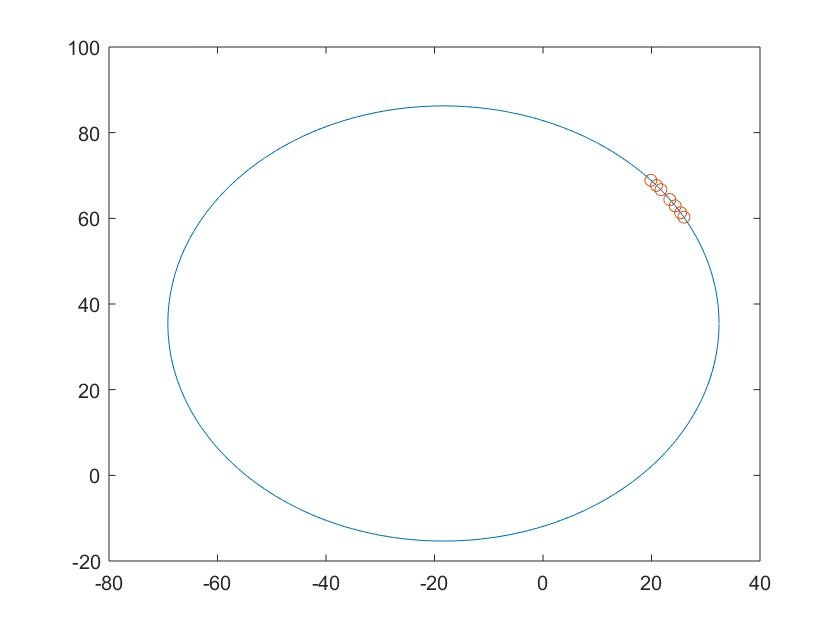
\includegraphics[width=9cm]{leastSq.jpg}
\end{figure}

\end{outputs}

\end{sol}








% 7.9
\section{Orthonormal Bases and the Gram Schmidt Process}

\begin{exer} (\textit{Gram-Schmidt Process})\\
Perform the Gram-Schmidt process to transform the vectors given in the Example 9 of the Section 7.9 to obtain an orthonormal basis for $\mathbb{R}^{3}$.

In this problem, use a nested loop and the MATLAB command \textit{norm}.
\end{exer}

\begin{sol}

\begin{verbatim}

w1 = [1 1 1]'; w2 = [0 1 1]'; w3 = [0 0 1]';
A = [w1 w2 w3]; % Construct a matrix A whose columns are w1, w2, and w3.
format short; [m, n] = size(A);
Q = zeros(m, n); % Initialize the matrix Q as an m*n zero matrix.

% Find an orthonormal basis for the column space of A.
for j = 1 : n
    v = A(:, j); % v begins as jth column of A.
    for i = 1 : (j-1)
        temp = Q(:, i)' * A(:, j);
        % Subtract each component of orthogonal projection of v
        % onto the subspace spanned by the vector Q(:, i).
        v = v - temp * Q(:, i);
    end
    Q(:, j) = v / norm(v); % Normalize v by its 2-norm.
end
disp('The orthonormal basis {q1,q2,q3} for R^3 from {w1,w2,w3} are as follows:')
disp('q1='); disp(Q(:,1)'); disp('q2='); disp(Q(:,2)'); disp('q3='); disp(Q(:,3)');
\end{verbatim}

\begin{outputs}
\begin{verbatim}

The orthonormal basis {q1,q2,q3} for R^3 from {w1,w2,w3} are as follows:
q1=
    0.5774    0.5774    0.5774

q2=
   -0.8165    0.4082    0.4082

q3=
   -0.0000   -0.7071    0.7071
\end{verbatim}
\end{outputs}

\end{sol}

\vspace{3mm}
\begin{exer}\label{GS} (\textit{Orthonormal Bases for the Four Fundamental Spaces})\\
Find orthonormal bases for the four fundamental spaces of the matrix


\begin{displaymath}
A = \left[\begin{array}{rrrr} 2& \hspace{2mm} -1& \hspace{5mm} 3&\hspace{4mm} 5\\ 4 & -3 & 1 & 3 \\ 3 & -2 & 3 & 4 \\ 4 & -1 & 15 & 17 \\ 7 & -6 & -7 & 0  \end{array} \right].
\end{displaymath}
\end{exer}

\begin{sol}

\begin{verbatim}

%--- The following is the function file 'GramSchmidt.m'. ---%

% Find an orthonormal basis for col(A) when A has full column rank.
function Q = GramSchmidt(A)

  [m, n] = size(A);

  % Initialize the matrix Q as an m*n zero matrix.
  Q = zeros(m, n); 

  for j = 1 : n
    % v begins as jth column of A.
    v = A(:, j); 
    for i = 1 : (j-1)
      temp = Q(:, i)' * A(:, j);
      % Subtract each component of orthogonal projection of v
      % onto the subspace spanned by the vector Q(:, i).
      v = v - temp * Q(:, i);
    end
    Q(:, j) = v / norm(v); % Normalize v by its 2-norm.
  end
end
% Q is an m*n matrix whose columns form an orthonormal basis for col(A).
\end{verbatim}

The following commands are performed in the command window of MATLAB.

\begin{verbatim}
A = [2 -1 3 5; 4 -3 1 3; 3 -2 3 4; 4 -1 15 17; 7 -6 -7 0];
format short;

% Find the reduced row echelon form of A.
rref_A = rref(A); 

% (1). Find an orthonormal basis for the row space of A.
% From the result of rref_A, the first three nonzero rows in rref_A form
% a basis for the row space of A.

% Construct a matrix R_A whose columns are a basis for the row space of A.
R_A = rref_A(1:3, :)';

% Find an orthonormal basis for the column space of R_A by Gram-Schmidt process,
% which is the same as finding an orthonormal basis for the row space of A.
Orth_R_A = GramSchmidt(R_A);

a1 = Orth_R_A(:, 1); a2 = Orth_R_A(:, 2); a3 = Orth_R_A(:, 3);

disp('An orthonormal basis {a1, a2, a3} for the row space of A is');
disp('a1 = '); disp(a1'); disp('a2 = '); disp(a2'); disp('a3 = '); disp(a3');

% (2). Find an orthonormal basis for the column space of A.
% From the result of rref_A, the first three columns of A are the pivot columns
% which form a basis for the column space of A.

% Construct a matrix C_A whose columns are a basis for the column space of A.
C_A = A(:, 1:3);

% Find an orthonormal basis for the column space of C_A by Gram-Schmidt process,
% which is the same as finding an orthonormal basis for the column space of A.
Orth_C_A = GramSchmidt(C_A);

b1 = Orth_C_A(:, 1); b2 = Orth_C_A(:, 2); b3 = Orth_C_A(:, 3);

disp('An orthonormal basis {b1, b2, b3} for the column space of A is');
disp('b1 = '); disp(b1'); disp('b2 = '); disp(b2'); disp('b3 = '); disp(b3');


% (3). Find an orthonormal basis for the null space of A.
% In addition, from the result of rref_A,
% we can easily see that {[-6 -7 0 1]'} is a basis for N(A).

% Construct a matrix N_A whose columns are a basis for the null space of A.
N_A = [-6 -7 0 1]';

% Find an orthonormal basis for the column space of N_A by Gram-Schmidt process,
% which is the same as finding an orthonormal basis for the null space of A.
Orth_N_A = GramSchmidt(N_A);

c1 = Orth_N_A(:, 1);
disp('An orthonormal basis {c1} for the null space of A is');
disp('c1 = '); disp(c1');

% (4). Find an orthonormal basis for the null space of A transpose.
[L U P] = lu(A);
temp = [0 0 0 0 1]';
\% Make L a square matrix of order 5.
L = [L temp]; 

% Make U have the same size of A.
U(5, :) = 0; 

% Then, we have P*A = L*U, which is the same result as above.
% Note that L^(-1)*P*A = U, where U is an upper triangular matrix.

E = L^(-1)*P;

% Since E = L^(-1)*P is a product of elementary matrices s.t. E*A=U,
% E represents a set of elementary row operations
% that makes A become a row echelon form U.

% ref_par_A is the resulting partitioned matrix [U E].
ref_par_A = [U E]; 

% From the result of ref_par_A, we can see that ref_par_A([4:5], [1:4]) = 0.
% Thus, the row vectors of E2 form a basis for null(A'),
% where E2 = ref_par_A([4:5], [5:9]).

% Construct a matrix N_Atrans whose columns are a basis for
% the null space of A transpose.
N_Atrans = ref_par_A(4:5, 5:9)';

% Find an orthonormal basis for the column space of N_Atrans by Gram-Schmidt process,
% which is the same as finding an orthonormal basis for the null space of A transpose.
Orth_N_Atrans = GramSchmidt(N_Atrans);

d1 = Orth_N_Atrans(:, 1); d2 = Orth_N_Atrans(:, 2);
disp('An orthonormal basis {d1, d2} for the null space of the transpose of A is');
disp('d1 = '); disp(d1'); disp('d2 = '); disp(d2');
\end{verbatim}

\begin{outputs}
\begin{verbatim}

An orthonormal basis {a1, a2, a3} for the row space of A is
a1 =
    0.1644         0         0    0.9864

a2 =
   -0.7446    0.6559         0    0.1241

a3 =
     0     0     1     0

An orthonormal basis {b1, b2, b3} for the column space of A is
b1 =
    0.2063    0.4126    0.3094    0.4126    0.7220

b2 =
    0.1873   -0.0887    0.0493    0.8378   -0.5027

b3 =
   -0.3699    0.5812    0.5878   -0.1321   -0.4029

An orthonormal basis {c1} for the null space of A is
c1 =
   -0.6470   -0.7548         0    0.1078

An orthonormal basis {d1, d2} for the null space of the transpose of A is
d1 =
    0.8649    0.3089         0   -0.3089   -0.2471

d2 =
    0.1936   -0.6234    0.7458   -0.1224    0.0512
\end{verbatim}
\end{outputs}

\end{sol}






% section 7.10


\section{$QR-$Decomposition; Householder Transformations}


\begin{exer}(\textit{$QR-$Decomposition})\\
\begin{enumerate}
\item[(a)] Make a function file \verb"myQR.m" to find a $QR$-decomposition of a given matrix. 
You may use your function file \verb"GS_process.m" from the \textbf{Exercise}~\ref{GS}.
\vspace{1mm}
\item[(b)] $$A=\begin{bmatrix} 1 & 1 & 1\\ 1& 0 & 2\\ 0 & 1& 2\end{bmatrix}.$$
Compare your result with the output produced by the MATLAB command \textit{qr}. 
\end{enumerate}
\end{exer}


\begin{sol}
\begin{verbatim}

%(a)
%--- This is a function file myQR.m ---%

function [Q R]=myQR(A)
 Q=GS_process(A);
 R=Q'*A;
end

%(b)
A=[1 1 1; 1 0 2; 0 1 2];
[Q1 R1]=myQR(A); [Q R]=qr(A);

disp('my QR result'); disp('Q');disp(Q1); disp('R');disp(R1);
disp('MATLAB QR result'); disp('Q');disp(Q); disp('R');disp(R);
\end{verbatim}

\begin{outputs}
\begin{verbatim}

my QR result
Q
    0.7071    0.4082   -0.5774
    0.7071   -0.4082    0.5774
         0    0.8165    0.5774
R
    1.4142    0.7071    2.1213
    0.0000    1.2247    1.2247
    0.0000   -0.0000    1.7321

MATLAB QR result
Q
   -0.7071    0.4082   -0.5774
   -0.7071   -0.4082    0.5774
         0    0.8165    0.5774
R
   -1.4142   -0.7071   -2.1213
         0    1.2247    1.2247
         0         0    1.7321
\end{verbatim}

\end{outputs}


\noindent The results are the same.
\end{sol}







% 7.11

\section{Coordinates with Respect to a Basis}

\begin{exer} (\textit{Transition Matrices between Two Different Bases})\\

\begin{enumerate}

\item[(a)] Confirm that $B_{1} = \{\mathbf{u}_{1}, \mathbf{u}_{2}, \mathbf{u}_{3}, \mathbf{u}_{4}, \mathbf{u}_{5}\}$ and $B_{2} = \{\mathbf{v}_{1}, \mathbf{v}_{2}, \mathbf{v}_{3}, \mathbf{v}_{4}, \mathbf{v}_{5}\}$ are bases for $\mathbb{R}^{5}$, and find the transition matrices $P_{\tiny{B_{1} \rightarrow B_{2}}}$ and $P_{\tiny{B_{2} \rightarrow B_{1}}}$, where

\begin{displaymath}
\begin{array}{lllllll}
\vspace{1mm} \mathbf{u}_{1} & = & (3, \hspace{1mm} 1, \hspace{1mm} 3, \hspace{1mm} 2, \hspace{1mm} 6) & \hspace{4mm} & \mathbf{v}_{1} & = & (2, \hspace{1mm} 6, \hspace{1mm} 3, \hspace{1mm} 4, \hspace{1mm} 2) \\ \vspace{1mm} \mathbf{u}_{2} & = & (4, \hspace{1mm} 5, \hspace{1mm} 7, \hspace{1mm} 2, \hspace{1mm} 4) & \hspace{4mm} & \mathbf{v}_{2} & = & (3, \hspace{1mm} 1, \hspace{1mm} 5, \hspace{1mm} 8, \hspace{1mm} 3) \\ \vspace{1mm} \mathbf{u}_{3} & = & (3, \hspace{1mm} 2, \hspace{1mm} 1, \hspace{1mm} 5, \hspace{1mm} 4) & \hspace{4mm} & \mathbf{v}_{3} & = & (5, \hspace{1mm} 1, \hspace{1mm} 2, \hspace{1mm} 6, \hspace{1mm} 7) \\ \vspace{1mm} \mathbf{u}_{4} & = & (2, \hspace{1mm} 9, \hspace{1mm} 1, \hspace{1mm} 4, \hspace{1mm} 4) & \hspace{4mm} & \mathbf{v}_{4} & = & (8, \hspace{1mm} 4, \hspace{1mm} 3, \hspace{1mm} 2, \hspace{1mm} 6) \\ \vspace{1mm} \mathbf{u}_{5} & = & (3, \hspace{1mm} 3, \hspace{1mm} 6, \hspace{1mm} 6, \hspace{1mm} 7) & \hspace{4mm} & \mathbf{v}_{5} & = & (5, \hspace{1mm} 5, \hspace{1mm} 6, \hspace{1mm} 3, \hspace{1mm} 4) \\
\end{array}
\end{displaymath}



\item[(b)] Find the coordinate matrices with respect to $B_{1}$ and $B_{2}$ of $\mathbf{w} = (1, \hspace{1mm} 1, \hspace{1mm} 1, \hspace{1mm} 1, \hspace{1mm} 1)$.

\end{enumerate}

\end{exer}



\begin{sol}
\begin{verbatim}

u1 = [3 1 3 2 6]'; v1 = [2 6 3 4 2]';
u2 = [4 5 7 2 4]'; v2 = [3 1 5 8 3]';
u3 = [3 2 1 5 4]'; v3 = [5 1 2 6 7]';
u4 = [2 9 1 4 4]'; v4 = [8 4 3 2 6]';
u5 = [3 3 6 6 7]'; v5 = [5 5 6 3 4]';

U = [u1 u2 u3 u4 u5]; 
V = [v1 v2 v3 v4 v5]; 

format short;

% Initialization.
P_B1B2 = zeros(5); 
P_B2B1 = zeros(5); 

for j = 1:5
  % Find the coordinate vector of U(:, j) in B1 with respect to B2.
  P_B1B2(:, j) = V\U(:, j);
  % Find the coordinate vector of V(:, j) in B2 with respect to B1.
  P_B2B1(:, j) = U\V(:, j);
end

disp('The transition matrix from B1 to B2 is'); disp(P_B1B2);
disp('The transition matrix from B2 to B1 is'); disp(P_B2B1);

w = [1 1 1 1 1]';

% Find the coordinate matrix of w with respect to B1.
w_B1 = U\w; 

% Find the coordinate matrix of w with respect to B2.
w_B2 = P_B1B2 * w_B1; 

disp('The coordinate matrix of w with respect to B1 is'); disp(w_B1');
disp('The coordinate matrix of w with respect to B2 is'); disp(w_B2');
\end{verbatim}


\begin{outputs}
\begin{verbatim}

The transition matrix from B1 to B2 is
   -0.4992   -0.2531    0.4843    1.8286   -0.2123
   -0.7830   -0.3679    0.1604   -0.8019   -0.5849
    1.3019    0.2925    0.4623    0.6887    1.4906
   -0.9096   -0.6116    0.1918   -0.2091   -1.4104
    1.4230    1.8082   -0.4591   -0.2044    1.8019

The transition matrix from B2 to B1 is
   -0.6889   -1.3556    0.6222    1.2667   -0.0444
    0.4067    0.3591    0.0278    1.2083    1.0873
    0.3151    1.2675    1.3444    1.6833    0.6540
    0.3615   -0.5433   -0.2056   -0.1417   -0.0746
    0.2571    0.9714   -0.2000   -1.8000   -0.3429

The coordinate matrix of w with respect to B1 is
   -0.0222    0.1508    0.1841   -0.0016   -0.0286

The coordinate matrix of w with respect to B2 is
    0.0653    0.0094    0.0566    0.0039    0.1053
\end{verbatim}
\end{outputs}

\end{sol}

% section8

\chapter{Diagonalization}

%8.1
\section{Matrix Representations of Linear Transformations}

\begin{exer}Let $T : \mathbb{R}^{5} \rightarrow \mathbb{R}^{3}$ be the linear operator given by the formula
$$T(x_{1}, x_{2}, x_{3}, \hspace{1mm} x_{4}, x_{5}) = (7x_{1}+12x_{2}-5x_{3}, \hspace{1mm} 3x_{1}+10x_{2}+13x_{4}+x_{5}, \hspace{1mm} -9x_{1}-x_{3}-3x_{5})$$
and let $B = \{\mathbf{v}_{1}, \hspace{1mm} \mathbf{v}_{2}, \hspace{1mm} \mathbf{v}_{3}, \hspace{1mm} \mathbf{v}_{4}, \hspace{1mm} \mathbf{v}_{5}\}$ and $B' = \{\mathbf{v}'_{1}, \hspace{1mm} \mathbf{v}'_{2}, \hspace{1mm} \mathbf{v}'_{3}\}$ be the bases for $\mathbb{R}^{5}$ and $\mathbb{R}^{3}$, respectively, in which $\mathbf{v}_{1} = (1, \hspace{1mm} 1, \hspace{1mm} 0, \hspace{1mm} 0, \hspace{1mm} 0)$, $\mathbf{v}_{2} = (0, \hspace{1mm} 1, \hspace{1mm} 1, \hspace{1mm} 0, \hspace{1mm} 0)$, $\mathbf{v}_{3} = (0, \hspace{1mm} 0, \hspace{1mm} 1, \hspace{1mm} 1, \hspace{1mm} 0)$, $\mathbf{v}_{4} = (0, \hspace{1mm} 0, \hspace{1mm} 0, \hspace{1mm} 1, \hspace{1mm} 1)$, $\mathbf{v}_{5} = (1, \hspace{1mm} 0, \hspace{1mm} 0, \hspace{1mm} 0, \hspace{1mm} 1)$, $\mathbf{v}'_{1} = (1, \hspace{1mm} 2, \hspace{1mm} -1)$, $\mathbf{v}'_{2} = (2, \hspace{1mm} 1, \hspace{1mm} 3)$, and $\mathbf{v}'_{3} = (1, \hspace{1mm} 1, \hspace{1mm} 1)$.

\vspace{2mm}
\begin{enumerate}

\item[(a)]
Find the matrix $[T]_{\tiny{B}', \tiny{B}}$.
\vspace{1mm}
\item[(b)]
For the vector $\mathbf{x} = (3, \hspace{1mm} 7, \hspace{1mm} -4, \hspace{1mm} 5, \hspace{1mm} 1)$, find $[\mathbf{x}]_{\tiny{B}}$ and use the matrix obtained in part~(a) to compute $[T(\mathbf{x})]_{\tiny{B}'}$.
\vspace{1mm}
\item[(c)] Find the factorization of [$T$] which is the standard matrix for the linear transformation $T$ using Formula (28) in Section 8.1.
\end{enumerate}

\end{exer}

\begin{sol}

\vspace{1mm}

\begin{enumerate}

\vspace{1mm}
\verb""
\item[(a)]
\begin{verbatim}
v1 = [1 1 0 0 0]'; v2 = [0 1 1 0 0]'; v3 = [0 0 1 1 0]';
v4 = [0 0 0 1 1]'; v5 = [1 0 0 0 1]';
nv1 = [1 2 -1]'; nv2 = [2 1 3]'; nv3 = [1 1 1]';

T = [7 12 -5 0 0; 3 10 0 13 1; -9 0 -1 0 -3];
B1 = [v1 v2 v3 v4 v5]; B2 = [nv1 nv2 nv3];
format short;

% Find the matrix representation with respect to the bases B1 and B2.
TB = T*B1;
TB1B2 = B2\TB;

disp('The matrix representation of T with respect to the basis B1 and B2 is');
disp(TB1B2);
\end{verbatim}



\begin{outputs}
\begin{verbatim}

The matrix representation of T with respect to the basis B1 and B2 is
   34.0000    5.0000  -22.0000  -11.0000   22.0000
   40.0000    2.0000  -40.0000  -25.0000   25.0000
  -95.0000   -2.0000   97.0000   61.0000  -65.0000
\end{verbatim}

\end{outputs}


\item[(b)]
\begin{verbatim}
% Find the coordinate vector of x with respect to the basis B1.
x = [3 7 -4 5 1]';  x_B1 = B1\x; 
disp('The coordinate vector of x with respect to the basis B is');
disp(x_B1');

% Find the coordinate vector of T(x) with respect to the basis B2.
Tx_B2 = TB1B2 * x_B1;
disp('The coordinate vector of T(x) with respect to the basis B'' is');
disp(Tx_B2');
\end{verbatim}



\begin{outputs}
\begin{verbatim}

The coordinate vector of x with respect to the basis B is
     9    -2    -2     7    -6

The coordinate vector of T(x) with respect to the basis B' is
  131.0000  111.0000 -228.0000
\end{verbatim}

\end{outputs}

\item[(c)]
\begin{verbatim}
% Transition matrix from B to the standard basis for R^n.
U=B1;

% Transition matrix from B' to the standard basis for R^m.
V=B2; 

T=[7 12 -5 0 0 ; 3 10 0 13 1; -9 0 -1 0 -3];

disp('V'); disp(V);
disp('TB1B2'); disp(TB1B2);
disp('inv(U)'); disp(inv(U));
disp('V*TB1B2*inv(U)');disp(V*TB1B2*inv(U));
disp('T'); disp(T);
\end{verbatim}


\begin{outputs}
\begin{verbatim}

V
     1     2     1
     2     1     1
    -1     3     1

TB1B2
   34.0000    5.0000  -22.0000  -11.0000   22.0000
   40.0000    2.0000  -40.0000  -25.0000   25.0000
  -95.0000   -2.0000   97.0000   61.0000  -65.0000

inv(U)
    0.5000    0.5000   -0.5000    0.5000   -0.5000
   -0.5000    0.5000    0.5000   -0.5000    0.5000
    0.5000   -0.5000    0.5000    0.5000   -0.5000
   -0.5000    0.5000   -0.5000    0.5000    0.5000
    0.5000   -0.5000    0.5000   -0.5000    0.5000

V*TB1B2*inv(U)
    7.0000   12.0000   -5.0000         0         0
    3.0000   10.0000         0   13.0000    1.0000
   -9.0000   -0.0000   -1.0000   -0.0000   -3.0000

T
     7    12    -5     0     0
     3    10     0    13     1
    -9     0    -1     0    -3
\end{verbatim}

\end{outputs}

\end{enumerate}
\end{sol}



%8.2 


\section{Similarity and Diagonalizability}


\begin{exer}

\begin{enumerate}
\item[(a)] Show that the matrix
$$A = \begin{bmatrix}-13&\hspace{1mm} -60&\hspace{1mm} -60\\ 10 & 42 & 40\\ -5 & -20 & -18 \end{bmatrix}$$
is diagonalizable by finding the nullity of $\lambda I - A$ for each eigenvalue $\lambda$ with the use of Theorem 8.2.11 in the Section 8.2.
\item[(b)] Find a basis for $\mathbb{R}^{3}$ consisting of eigenvectors of $A$.
\end{enumerate}
\end{exer}

\begin{sol}
\verb""
\begin{enumerate}
\item[(a)]
\begin{verbatim}
% For the exact computation of the eigenvalues, 
% we use symbolic computation. 

% Set A as a symbolic matrix.
A = sym([-13 -60 -60; 10 42 40; -5 -20 -18]); 

n = length(A);

% Find the eigenvalues of A by using the command eig.
eigenvalues = eig(A); 

for j = 1 : n
    fprintf('The eigenvalue lambda is '); disp(eigenvalues(j));
    
    % nullity(lambda*I - A) = n - rank(lambda*I - A);
    nullity = n - rank((eigenvalues(j) * eye(n)) - A);
    
    fprintf('The nullity of (lambda*I - A) is '); disp(nullity);
end

% Since the geometric multiplicity of each eigenvalue of A 
% is the same as the algebraic multiplicity,
% by the Theorem 8.2.11, A is diagonalizable.
\end{verbatim}

\begin{outputs}

\begin{verbatim}

The eigenvalue lambda is 2
The nullity of (lambda*I - A) is      2
The eigenvalue lambda is 2
The nullity of (lambda*I - A) is      2
The eigenvalue lambda is 7
The nullity of (lambda*I - A) is      1
\end{verbatim}

\end{outputs}


\item[(b)]
\begin{verbatim}
% Since the eigenvalue = 2 of A has the multiplicity = 2, 
% find two linearly independent eigenvectors of A corresponding to lambda = 2.

%Find a basis for the null space of (2*I-A).
eigvec12=null((2 * eye(n)) - A);

% Since the eigenvalue = 7 of A has the multiplicity = 1, 
% find an eigenvector of A corresponding to lambda = 7.

%Find a basis for the null space of (7*I-A).
eigvec3=null((7 * eye(n)) - A);

p1 = eigvec12(:, 1); p2 = eigvec12(:, 2); p3 = eigvec3(:, 1); 

% By the Theorem 8.2.7, since the eigenvectors corresponding to 
% distinct eigenvalues are linearly independent,
% the three obtained eigenvectors {p1, p2, p3} form a basis for R^{3}.

disp('A basis {p1, p2, p3} for R^{3} consisting of the eigenvectors of A is');
fprintf('p1 ='); disp(p1'); 
fprintf('p2 ='); disp(p2'); 
fprintf('p3 ='); disp(p3');
\end{verbatim}


\begin{outputs}

\begin{verbatim}

A basis {p1, p2, p3} for R^{3} consisting of the eigenvectors of A is
p1 =[ -4, 1, 0]
p2 =[ -4, 0, 1]
p3 =[ 3, -2, 1]
\end{verbatim}
\end{outputs}


\end{enumerate}
\end{sol}










% 8.3
\section{Orthogonal Diagonalizability; Functions of a Matrix}


\begin{exer}
\begin{enumerate}
Let
$$A=\begin{bmatrix}\frac{1}{2} & 0 & \frac{3}{2} & 0 \\ 0 & \frac{1}{2} & 0 & \frac{3}{2} \\ \frac{3}{2} & 0 & \frac{1}{2} & 0 \\ 0 & \frac{3}{2} & 0 & \frac{1}{2}\end{bmatrix}.$$
\begin{enumerate}
\item[(a)]
Find a matrix $P$ that orthogonally diagonalizes the matrix $A$. You may use the MATLAB command \textit{eig} and perform the Gram-Schmidt process. Use your result to find a diagonal matrix $D$ satisfying $A=PDP^{T}$.
\vspace{1mm}
\item[(b)]
Confirm that the matrix $A$ satisfies its characteristic equation, in accordance with the Cayley-Hamilton theorem. You may use the symbolic object to find the characteristic polynomial and use the MATLAB command \textit{coeffs} to find the coefficient of obtained characteristic polynomial.
\vspace{1mm}
\item[(c)]
%Compute $e^{A}$ as given in Example 5 of Section 8.3. Compare the result with the MATLAB syntax \textit{exp(A)}.
%\item[(d)]
Find the spectral decomposition of $A$.
\end{enumerate}
\end{enumerate}
%\end{exer}


\begin{sol}
\verb""
\begin{enumerate}
\item[(a)]
\begin{verbatim}
A=[1/2 0 3/2 0; 0 1/2 0 3/2; 3/2 0 1/2 0; 0 3/2 0 1/2];

% V: eigen vector, D: eigen value
[V D]=eig(A);

% Gram-Schmidt process
P=GS_process(V);    
disp('P is'); disp(P);
disp('D is'); disp(D);
disp('P_transpose is'); disp(P');
disp('P*D*P_transpose is'); disp(P*D*P');
disp('A is'); disp(A);
\end{verbatim}


\begin{outputs}

\begin{verbatim}

P is
   -0.7071         0         0   -0.7071
         0    0.7071    0.7071         0
    0.7071         0         0   -0.7071
         0   -0.7071    0.7071         0

D is
    -1     0     0     0
     0    -1     0     0
     0     0     2     0
     0     0     0     2

P_transpose is
   -0.7071         0    0.7071         0
         0    0.7071         0   -0.7071
         0    0.7071         0    0.7071
   -0.7071         0   -0.7071         0

P*D*P_transpose is
    0.5000         0    1.5000         0
         0    0.5000         0    1.5000
    1.5000         0    0.5000         0
         0    1.5000         0    0.5000

A is
    0.5000         0    1.5000         0
         0    0.5000         0    1.5000
    1.5000         0    0.5000         0
         0    1.5000         0    0.5000
\end{verbatim}

\end{outputs}


\item[(b)]
\begin{verbatim}
% Symbolic variable lambda
syms lambda;    

% Characteristic polynomial
char_poly=det(lambda*eye(size(A))-A); 

% Expand the characteristic polynomial cf. simplify
polynomial=expand(char_poly);   

% Coefficients extraction
coeff=coeffs(polynomial); 

% According to the descending order of lambda degree
coefficient=coeff(end:-1:1); 

 % Compute the matrix polynomial
poly_A=polyvalm(double(coefficient), A);

disp('Coefficients of the matrix characteristic polynomial is');
disp(double(coefficient));
disp('Matrix characteristic polynomial is'); disp(poly_A);
\end{verbatim}



\begin{outputs}

\begin{verbatim}

Coefficients of the matrix characteristic polynomial is
     1    -2    -3     4     4

Matrix characteristic polynomial is
     0     0     0     0
     0     0     0     0
     0     0     0     0
     0     0     0     0
\end{verbatim}
\end{outputs}

\item[(c)]
\begin{verbatim}
[V D]=eig(A);
sum_A=0;
for i=1:size(A,1);
  % spectral decomposition
  sum_A=sum_A+D(i,i)*V(:,i)*V(:,i)'; 

  fprintf('lambda_%d is %f \n', i, D(i,i));
  fprintf('corresponding u_%d is \n', i);
  disp(V(:,i));
end

disp('spectral decomposition of A is'); disp(sum_A);
disp('A is'); disp(A);
\end{verbatim}


\begin{outputs}

\begin{verbatim}
lambda_1 is -1.000000
corresponding u_1 is
   -0.7071
         0
    0.7071
         0

lambda_2 is -1.000000
corresponding u_2 is
         0
    0.7071
         0
   -0.7071

lambda_3 is 2.000000
corresponding u_3 is
         0
    0.7071
         0
    0.7071

lambda_4 is 2.000000
corresponding u_4 is
   -0.7071
         0
   -0.7071
         0

spectral decomposition of A is
    0.5000         0    1.5000         0
         0    0.5000         0    1.5000
    1.5000         0    0.5000         0
         0    1.5000         0    0.5000

A is
    0.5000         0    1.5000         0
         0    0.5000         0    1.5000
    1.5000         0    0.5000         0
         0    1.5000         0    0.5000
\end{verbatim}
\end{outputs}
\end{enumerate}
\end{sol}


\end{exer}








% 8.4



\section{Quadratic Forms}


\begin{exer}(\textit{Cholesky Factorization})\\
In this problem, we find a Cholesky factorization of the Hilbert matrix
$$A=\begin{bmatrix}1 & 1/2 & 1/3 & 1/4\\ 1/2 & 1/3 & 1/4 & 1/5 \\ 1/3 & 1/4 & 1/5 & 1/6 \\ 1/4 & 1/5 & 1/6 & 1/7\end{bmatrix}.$$
To generate the Hilbert matrix, you may use the MATLAB command \textit{hilb}.
\begin{enumerate}
\item[(a)] Show that $A$ is positive definite symmetric matrix by finding its eigenvalues and the MATLAB command \textit{issymmetric}.
\vspace{1mm}
\item[(b)] Make a function file \verb"ludecomp.m" to find the $LU$-decomposition of an invertible $n \times n$ matrix $A$ such that $A$ can be reduced to row echelon form by Gaussian elimination without row interchanges. You may refer to the four steps given in Page 157. Check your result by applying this function for the matrix given in the Example 2 of the Section 3.7.
\vspace{1mm}
\item[(c)] Referring to the Section 3.7, find the $LDU$-factorization of $A$ from an $LU$-factorization of $A$ by \verb"ludecomp.m".
\vspace{1mm}
\item[(d)] From the $LDU$-factorization of $A$ obtained in (c), find a Cholesky factorization $A=R^{T}R$, where $R$ is upper triangular.
\vspace{1mm}
\item[(e)] Use the MATLAB command \textit{chol} to find a Cholesky factorization of $A$. Compare it with the result obtained in (d).
\end{enumerate}


\begin{sol}
\verb""
\begin{enumerate}
\item[(a)]
\begin{verbatim}
format rat;
A=hilb(4);

eig_val=eig(A);
if all(eig_val>0) && issymmetric(A)==1
    disp('Given matrix A is'); disp(A);
    disp('A is symmetric and positive definite matrix.');
    fprintf('eigen value of A is '); disp(eig_val');
end
\end{verbatim}

\begin{outputs}
\begin{verbatim}
Given matrix A is
       1              1/2            1/3            1/4
       1/2            1/3            1/4            1/5
       1/3            1/4            1/5            1/6
       1/4            1/5            1/6            1/7

A is symmetric and positive definite matrix.
eigen value of A is    66/682507   101/14989   262/1549   3500/2333
\end{verbatim}
\end{outputs}



\item[(b)]
\begin{verbatim}
%--- This is a function file 'ludecomp.m' ---%
function [L, U] = ludecomp(A)

% The number of rows and columns of the matrix A.
[nrow, ncol] = size(A); 

% Initialization of U and L.
U = A; L = eye(ncol); 

% Forward Elimination %
for i=1:nrow
    % Find the first nonzero entry of the ith row.
    for k=i:ncol
        if U(i,k) ~= 0
            break % Terminates the execution of the loop.
        end
    end
    temp1 = U(i,k); % Save U(i,k) in temp.
    U(i,:) = (1/temp1) * U(i,:);
    % Normalize the pivot (i,k)-entry by 1 to the ith row.
    L(i,i) = (1/temp1)^(-1);
    % Place the reciprocal of the multiplier in that position in U.
        if i ~= nrow
        for j=(i+1):nrow
            temp2 = U(j,k); % Save U(j,k) in temp2.
            U(j,:) = ((-temp2) * U(i,:)) + U(j,:);
            % Add minus (j,k)-entry times the ith row to the jth row
            L(j,i) = -(-temp2);
            % Place the negative of the multiplier in that position in U.
        end
    end
end
\end{verbatim}


\item[(c)]
\begin{verbatim}
% LU-factorization of A without row interchanges
[L, U] = ludecomp(A); 

% From an LU-factorization of A, we can find the LDU-factorization of A,
% by appropriate normalization of L.
D = diag(diag(L));

for i = 1:4
    L(:, i) = L(:, i)./L(i, i);
end

disp('The LDU-factorization of A is');
disp('L = '); disp(L); disp('D = '); disp(D); disp('U = '); disp(U);

\end{verbatim}


\begin{outputs}
\begin{verbatim}

The LDU-factorization of A is
L =
       1              0              0              0
       1/2            1              0              0
       1/3            1              1              0
       1/4            9/10           3/2            1

D =
       1              0              0              0
       0              1/12           0              0
       0              0              1/180          0
       0              0              0              1/2800

U =
       1              1/2            1/3            1/4
       0              1              1              9/10
       0              0              1              3/2
       0              0              0              1
\end{verbatim}
\end{outputs}


\item[(d)]
\begin{verbatim}
% From the LDU-factorization of A, find the Cholesky factor.
R1 = (L*sqrt(D))';
disp('The Cholesky factor R1 from the LDU-factorization of A is'); 
disp(R1);
\end{verbatim}

\begin{outputs}
\begin{verbatim}

The Cholesky factor R1 from the LDU-factorization of A is
       1              1/2            1/3            1/4
       0            390/1351       390/1351       351/1351
       0              0            317/4253       323/2889
       0              0              0            153/8096
\end{verbatim}
\end{outputs}


\item[(e)]
\begin{verbatim}
% Find a Cholesky factorization of A by using the MATLAB command.
R2 = chol(A);
disp('The Cholesky factor R2 from the MATLAB command chol is'); 
disp(R2);
\end{verbatim}


\begin{outputs}
\begin{verbatim}

The Cholesky factor R2 from the MATLAB command chol is
       1              1/2            1/3            1/4
       0            390/1351       390/1351       351/1351
       0              0            317/4253       323/2889
       0              0              0            153/8096
\end{verbatim}
\end{outputs}
\end{enumerate}
\end{sol}

\end{exer}



\end{document}